%%%%%%%%%%%%%%%%%%%%%%%%%%%%%%%%%%%%%%%%%%%%%%%%%%%%%%%%%%%%
% Pedro Brandão's trial to get a template for thesis for students
% Used the upthesis from Fernando Silva (see upthesis).
% See also the packages file.
% 2014/07/07 First draft
% 2014/07/21 
%  pbrandao: added the list of listings (it should produce portuguese name if
%           babel is set to portuguese, see packages.tex). Changed usepackage of babel
%           to be before input packages.tex to allow test

%
%%%%%%%%%%%%%%%%%%%%%%%%%%%%%%%%%%%%%%%%%%%%%%%%%%%%%%%%%%%%


% makes all pages the height of the text on that page. No extra vertical space is added.
\raggedbottom 
% setting it to report will remove the blank pages before each chapter
\documentclass[11pt,a4paper,twoside]{book}

\usepackage[numbers,sort&compress]{natbib}

%%%%%%%%%%%%%%%%%%%%%%%%%%%%%%%%%%%%%%%%%%%%%%%%%%%%%%%%%%%%
%%%   Packages that need to be configured for the thesis
%%%%%%%%%%%%%%%%%%%%%%%%%%%%%%%%%%%%%%%%%%%%%%%%%%%%%%%%%%%%

% Language settings
% use UKenglish for UK or leave blank for US English
% it will also change the names for some of the chapters (list of tables, figures, content,
\usepackage[UKenglish]{babel}
%\usepackage[portuguese]{babel}

%%%%%%%%%%%%%%%%%%%%%%%%%%%%%%%%%%%%%%%%%%%%%%%%%%%%%%%%%%%%
%%%   Packages uses language definitions
% see file below for more packages and settings
%%%%%%%%%%%%%%%%%%%%%%%%%%%%%%%%%%%%%%%%%%%%%%%%%%%%%%%%%%%%
\usepackage{upthesis}
\usepackage{tablefootnote}

\usepackage{epigraph, varwidth}

\setlength\epigraphwidth{8cm}
\setlength\epigraphrule{0pt}
\usepackage{subcaption}


\usepackage{array} % For better column formatting
\usepackage{ragged2e} % For text wrapping
\usepackage{longtable}
\usepackage{multirow}
\usepackage[
%backref={section},
%pagebackref, % for getting references to the page where the citation is (in the biblio)
pdfpagelabels=false
]{hyperref}


\hypersetup{pdftitle={Study for the Development of Lens Calibration Algorithm}, %nao suporta acentos
   pdfkeywords ={palavras chave},
   pdfsubject = {assunto},
	bookmarksnumbered=true,
   pdfauthor ={João Pedro da Silva Brito}, % see other options on manual (can be page) needs empty line on bibitem
   plainpages=false, 
   pdfborder={0 0 0},
   colorlinks,%colorlinks=false,
   breaklinks=true,
	%linktocpage= false, make page number, not text, be link on TOC, LOF and LOT 
	%hyperindex=true 	% Makes the page numbers of index entries into hyperlinks. Relays on unique page anchors (pageanchor) 
% see for colors http://mirror.ctan.org/macros/latex/contrib/xcolor/xcolor.pdf
   linkcolor= blue, %RedViolet, %MidnightBlue,% BlueViolet,%Sepia, % Color for normal internal links.
   %anchorcolor=black,% Color for anchor text.
   citecolor= blue,% Color for bibliographical citations in text.
   %filecolor=cyan% Color for URLs which open local files.
   %menucolor=red% Color for Acrobat menu items.
   %runcolor=filecolor% Color for run links (launch annotations).
   urlcolor=blue,% Color for linked URLs.
}
%use the same style for \url as the text
% from http://en.wikibooks.org/wiki/LaTeX/Hyperlinks#Customization
\urlstyle{same}

\makeatletter
\renewcommand*{\cleardoublepage}{\clearpage\if@twoside \ifodd\c@page\else
\thispagestyle{empty}
\if@twocolumn\hbox{}\newpage\fi\fi\fi}
\makeatother
\usepackage{setspace}
\setstretch{1.5}
\usepackage{arydshln}
\usepackage{pdfpages}
\usepackage[super]{nth}
\usepackage{hyperref}
\hypersetup{
    colorlinks=true,
    linkcolor=blue,
    filecolor=magenta,      
    urlcolor=cyan,
    pdftitle={Study for the Development of Lens Calibration Algorithm},
    pdfpagemode=FullScreen,
    }

\urlstyle{same}


\setcounter{tocdepth}{3}
\setcounter{secnumdepth}{3}

%\usepackage{emoji}
\usepackage{tikz}
\usepackage{graphicx}
%\usepackage[table,xcdraw]{xcolor}
\usepackage{lscape}
\usepackage{booktabs}

\newcommand{\red}{\tikz\draw[red,fill=red] (0,0) circle (1ex);}
\newcommand{\yellow}{\tikz\draw[yellow,fill=yellow] (0,0) circle (1ex);}
\newcommand{\green}{\tikz\draw[green,fill=green] (0,0) circle (1ex);}


\begin{document}



\includepdf[pages=1]{Chapters/thesis}
\cleardoublepage

\includepdf[pages=2]{Chapters/thesis}
\cleardoublepage


 % \quotepage{Random Usuário do Twitter}
 % {Levanta a cabeça se não a coroa cai %\emoji{crown} 
 % TEM QUE SE COMPILAR COM LUALATEX O EMOJI (VERIFICAR QUE NÃO ESTRAGA O RESTO DO DOC)}

\beforepreface%

\prefacesection{Acknowledgements}



\prefacesection{Abstract}

\noindent WTVision, a business that specializes in real-time graphics and augmented reality solutions for the broadcast and entertainment industries, provided a corporate setting for this internship. With the use of WTVision's technology, immersive experiences that demand a high degree of visual accuracy and precision are produced. Accurate recreation of a camera lens distortion in a virtual environment is a major problem in these settings and an accurante determinatation of distortion coeffients is mandatory for recreating immersive AR experiences.

\noindent It's important to clarify that in augmented and virtual reality applications, where seamless alignment between virtual features and real-world visuals is necessary to deliver an immersive user experience, the aim is not to minimize the camera's distortion effect. Instead, the goal is to make the virtual world look geometrically aligned to the real world does. However, current calibration methods are extremely time-consuming and require meticulous manual adjustments at different zoom and focus levels. Manual calibration typically takes between 4 to 8 hours and is heavily reliant on human factors, increasing the likelihood of errors.

\noindent The objective of this project is to create a lens calibration algorithm that optimizes and automates the procedure, cutting the overall calibration time down to about 30 minutes while maintaining accuracy. The suggested approach makes better use of cutting-edge methods like image analysis and machine learning to fix distortion issues. The study encompasses a thorough examination of current calibration techniques, the creation and modeling of a novel algorithm, and exhaustive experimentation on various types of lens under different circunstances.

\noindent The study's findings should greatly enhance the workflow for calibration teams by enabling faster, more accurate calibrations with less need for human intervention. The suggested method could significantly increase productivity in fields where accurate camera lens calibration is essential, especially for augmented and virtual reality applications.

\prefacesection{Resumo}
\noindent A WTVision é uma empresa especializada em soluções de gráficos em tempo real e realidade aumentada para a indústria de transmissão e entretenimento. A tecnologia da WTVision permite criar experiências imersivas que exigem um alto grau de precisão e exatidão visual. Um dos principais desafios nesses cenários é a recriação precisa da distorção de lentes de câmera em um ambiente virtual, sendo essencial a determinação acurada dos coeficientes de distorção para a criação de experiências imersivas de realidade aumentada.

\noindent É importante esclarecer que, em aplicações de realidade aumentada e virtual, onde o alinhamento perfeito entre elementos virtuais e imagens do mundo real é essencial para proporcionar uma experiência imersiva, o objetivo não é minimizar a distorção da câmera. Em vez disso, busca-se garantir que o mundo virtual esteja geometricamente alinhado com o mundo real. No entanto, os métodos atuais de calibração são extremamente demorados e exigem ajustes manuais meticulosos em diferentes níveis de zoom e foco. A calibração manual geralmente leva entre 4 a 8 horas e depende fortemente de fatores humanos, aumentando a probabilidade de erros.

\noindent O objetivo deste projeto é desenvolver um algoritmo de calibração de lentes que otimize e automatize o procedimento, reduzindo o tempo total de calibração para cerca de 30 minutos, sem comprometer a precisão. A abordagem proposta faz uso de técnicas avançadas, como análise de imagens e aprendizado de máquina, para corrigir problemas de distorção. O estudo abrange uma análise detalhada dos métodos atuais de calibração, o desenvolvimento e modelagem de um novo algoritmo e experimentações extensivas com diferentes tipos de lentes sob diversas condições.

\noindent Os resultados deste estudo devem melhorar significativamente o fluxo de trabalho das equipes de calibração, permitindo calibrações mais rápidas e precisas, com menor necessidade de intervenção humana. O método proposto pode aumentar substancialmente a produtividade em áreas onde a calibração precisa de lentes de câmera é essencial, especialmente em aplicações de realidade aumentada e virtual.



%\dedicationpage{Dedico a \ldots}

% end of thesis preamble
\afterpreface%

%% main tex here
%% By putting the chapter names here, one can just comment the content in the chapters 
%% and produce a pdf with the correct chapter number.
%% If you want further configurability you can use subfiles package
%% https://www.ctan.org/pkg/subfiles

\chapter{Introduction}\label{chap:intro}

\section{Context}\label{sec:context}

\noindent Precise and dependable systems have become essential in an era where enterprises are driven toward more accuracy and efficiency by technology breakthroughs. The broadcast and entertainment industries have experienced significant expansion among these sectors due to the growing demand for immersive visual experiences enabled by \ac{AR} and \ac{VR} technologies. These innovations are transforming the way people consume material by providing them with interactive and captivating experiences. WTVision, a top business that specializes in real-time graphics and augmented reality solutions for many industries, is at the vanguard of this transformation.


\noindent The dynamic, aesthetically captivating settings that WTVision's technology helps creating for live broadcasts, sporting events, and virtual productions are essential. Achieving the desired level of realism that viewers anticipate requires a smooth transition between \ac{CGI} and real-world sights. But there are several obstacles in the way of reaching this level of visual accuracy, especially when it comes to camera lens calibration, which is essential to collecting real-world situations and matching them with virtual features.


\noindent To reduce image distortion, a frequent problem brought on by the physical characteristics of lenses, lens calibration is essential. In AR and VR settings, distortion can cause errors that impair the user experience. This difficulty is increased in apps that use varying zoom and focus settings since each one needs to be precisely calibrated in order to guarantee proper alignment of the virtual and real elements. At the moment, the labor- and time-intensive process of calibrating camera lenses takes four to eight hours and involves manual adjustments. The repetitive nature of the work and human mistake both make the process even more inefficient.


\noindent The limits of manual calibration approaches become more evident as the demand for AR and VR applications grows, especially in live broadcasts and virtual events. An automated solution that can speed up the calibration process and increase accuracy while decreasing time is desperately needed as a result of this. In light of this, the project's goal is to create a lens calibration algorithm that makes use of cutting-edge tools like image analysis and machine learning. The aim is to achieve maximum precision while radically reducing the time needed for the calibration process through automation and optimization.


\noindent The suggested method has the ability to greatly increase workflow efficiency in sectors that depend on accuratly determined camera lens distortion coefficients by resolving these issues. WTVision is ideally positioned to spearhead this endeavor and shape the future of immersive broadcast experiences because to its experience with real-time graphics and augmented reality technologies. If this effort is successful, it could improve the visual quality of AR and VR material and establish new guidelines for lens calibration procedures in a variety of businesses.
\section{wTVision}\label{sec:wTVision}


\noindent wTVision is a company \cite{wtvision} specialized in creating integrated broadcasting solutions, focusing on software development, graphics design and live operations.
\noindent Founded in 2001 and part of the Mediapro Group, wTVision has become a significant player in the broadcasting industry. The company provides a wide range of services, including real-time graphics, playout automation, augmented reality, virtual productions, and data distribution, serving live broadcasts, sports events, election coverage, entertainment shows, and news programs.


\noindent The company became one of the main real-time on-air graphics and playout automation providers due to its flexible solutions that can be integrated with multiple major graphics engines on the market. From small one time broadcasts to some of the most important competitions, wTVision takes part in more than 7 000 broadcasts annually and has experience in more than 120 countries. 
wTVision has hundreds of specialists around the globe and offices in Portugal, Spain, Belgium, Brazil, Bolivia, United Arab Emirates, India and USA.

\noindent Given that the sports industry is a primary focus for the company, and football is the dominant market in Portugal and many other countries, artificial intelligence and computer vision present a wide range of new opportunities to be explored. As a result, this topic has been increasingly investigated by researches over the past years. 


\section{Problem Definition and Internship Goals}\label{sec:intern_goals}

\noindent This section presents a clear description of the current problem. This section will use the following fundamental concepts: \textbf{Augmented Reality \ac{AR}}, \textbf{lens distortion} and the \textbf{$R^3$ software}. A detailed explanation of each can be found in chapter \ref{chap:state_art}.

\noindent wTVision developed the \( R^3 \) software for creating virtual environments and integrating virtual objects into real scenes. This software enables augmented reality experiences by seamlessly introducing virtual elements into live footage. However, it does not account for lens distortion, meaning virtual objects remain undistorted while the real scene may exhibit natural optical warping. The challenge of this project is not to correct lens distortion but to accurately replicate it within virtual environments, ensuring a more realistic and cohesive augmented reality experience.

\noindent The limitations of the $R^3$ software, including its reliance on operator expertise, time-intensive calibration process, and lack of automation for dynamic zoom and focus adjustments, underscore the need for a more efficient solution.

\noindent This thesis aims to improve the calibration process by:
\begin{itemize}
    \item Reducing reliance on operator expertise.
    \item Automating the process to decrease calibration time.
\end{itemize}

\subsection{Current Solution} \label{sec:current_solution}

\noindent This section focuses on wTVision’s current solution for calibrating a virtual environment, which
involves using the $R^3$
software to distort the virtual environment to match the distortion observed
in the real world.

\noindent While this approach is effective, the quality of the calibration—and, consequently, the realism of the virtual overlays—relies heavily on the calibration operator’s experience and expertise. Additionally, it is a time-consuming process, typically taking between 4 to 6 hours.

\subsubsection*{Detailed Calibration Process}

\noindent The calibration process involves determining the calibration coefficients in the following order:

\begin{itemize}
    \item Center-shift
    \item Field of View
    \item \( k_1 \) (radial distortion)
    \item \( k_2 \) (radial distortion at the edges)
    \item Nodal Point
\end{itemize}

\subsubsection*{Calibration Preparation}

\noindent Before starting the calibration process, the dimensions and coordinates of a real object on a real scene must be defined and provided to the $R^3$ software. This step can be completed either before or after the center-shift calibration. The following steps outline the calibration process for each coefficient:

\begin{enumerate}
    \item \textbf{Center-Shift:}  Align the virtual object with the real object at the center of the image.
    Adjust the central-shift coefficient until they match at minimum and maximum zoom levels.
    Intermediate values are interpolated.
    Figure \ref{fig:Cone} illustrates the current process for calibrating this coefficient. First, a real-world
    image with a reference point is required; typically, a phone light is used to produce the white circle in the
    image shown at the top of Figure \ref{fig:Cone}. Next, a cone is introduced. This cone does not
    need any specific characteristics other than having a pointy end. The center-shift is then
    adjusted, as depicted, until the pointy end of the cone aligns with the center of the white
    circle of light. After achieving this alignment, zoom in and verify that the pointy end
    remains at the center of the circle of light. If not, readjust the center-shift accordingly.

    Figure \ref{fig:Cone} illustrates the current process for calibrating this coefficient. First, a real-world image with a reference point is required; typically, a phone light is used to produce the image shown at the top of Figure \ref{fig:Cone}. Next, a cone is introduced. This cone does not need any specific characteristics other than having a pointy end. The center-shift is then adjusted, as depicted, until the pointy end of the cone aligns with the center of the white circle of light. After achieving this alignment, zoom in and verify that the pointy end remains at the center of the circle of light. If not, readjust the center-shift accordingly.
    
    \begin{figure}[h]
    \centering
    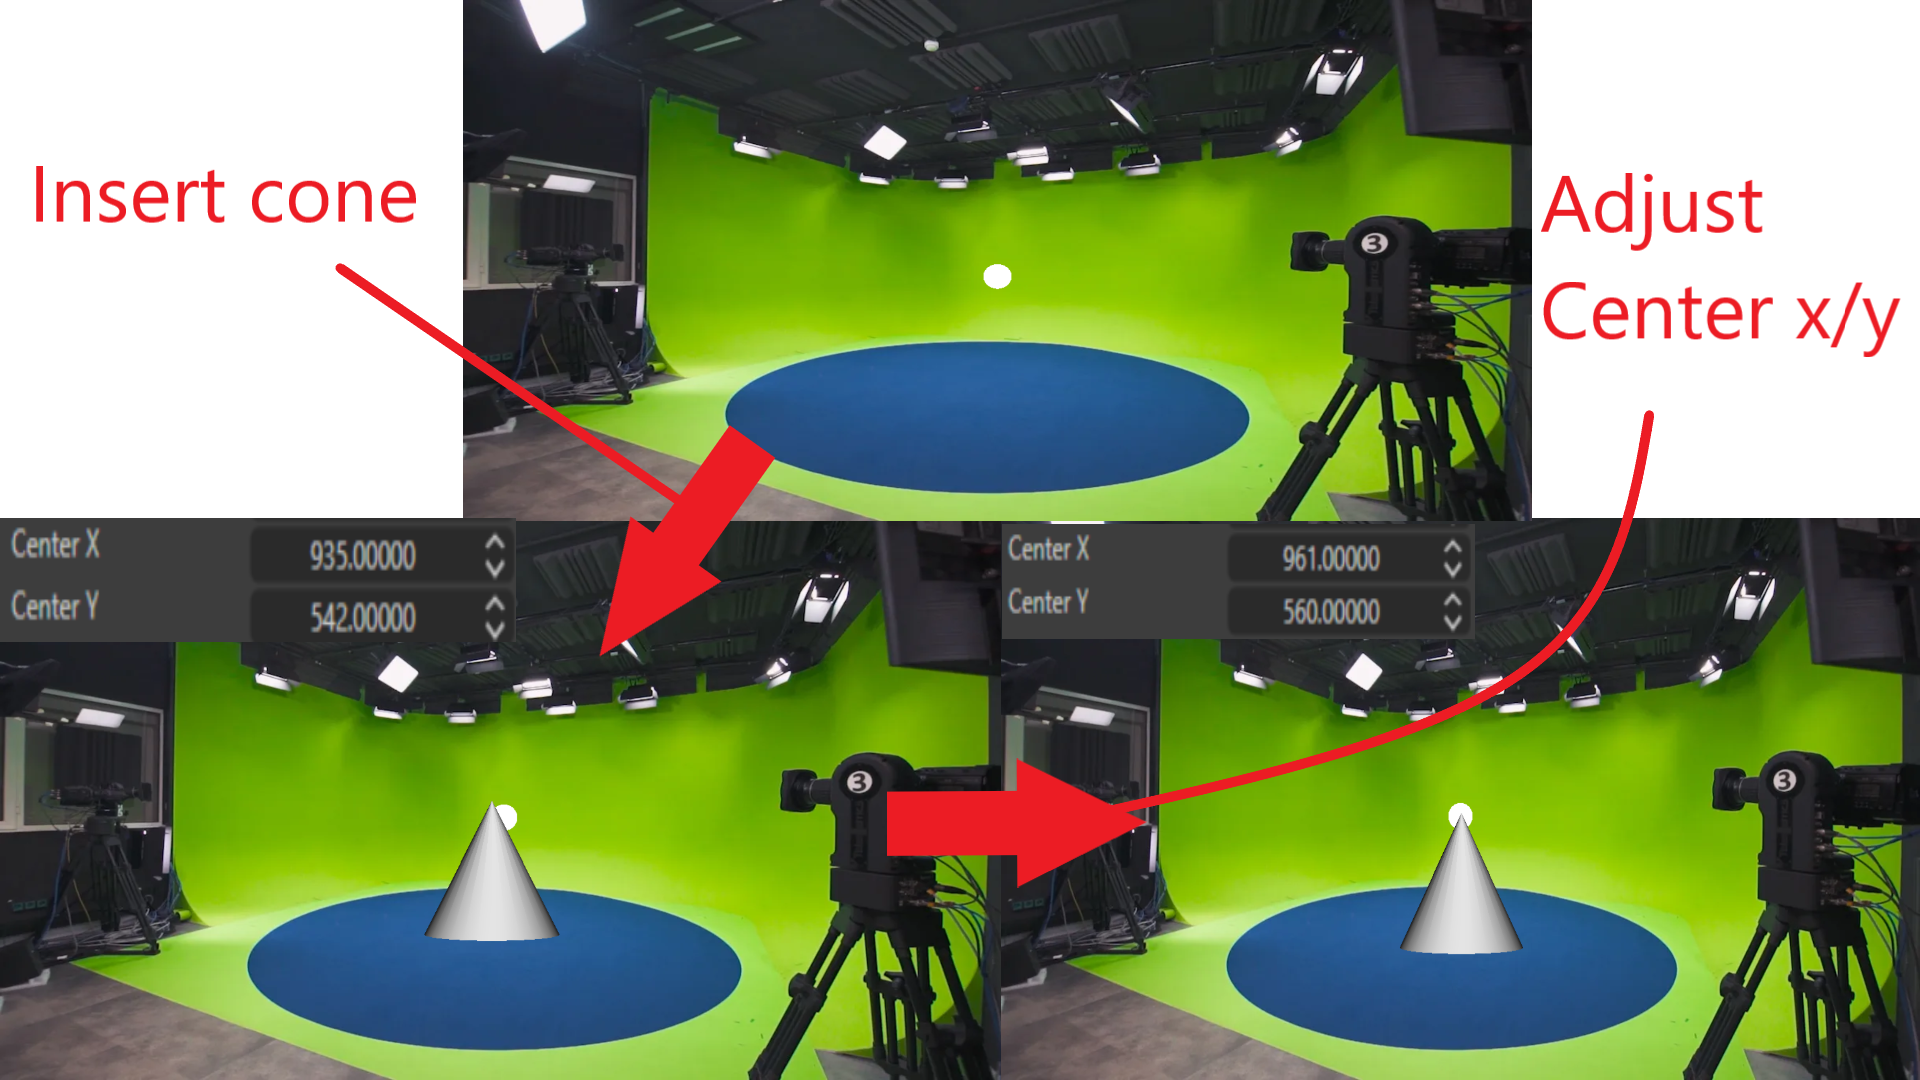
\includegraphics[width=\textwidth]{Images/01intro/Cone.png}
    \caption{Center shift calibration procedure example}
    \label{fig:Cone}
    \end{figure}
    
    
    
    \item \textbf{Field of View:} Move the real object (red square) off-center, then align the virtual object with the real object. Repeat this process for seven zoom levels to capture variations in distortion. Figure \ref{fig:FoV_pro} illustrates the calibration procedure for a FoV.

    \begin{figure}[h]
    \centering
    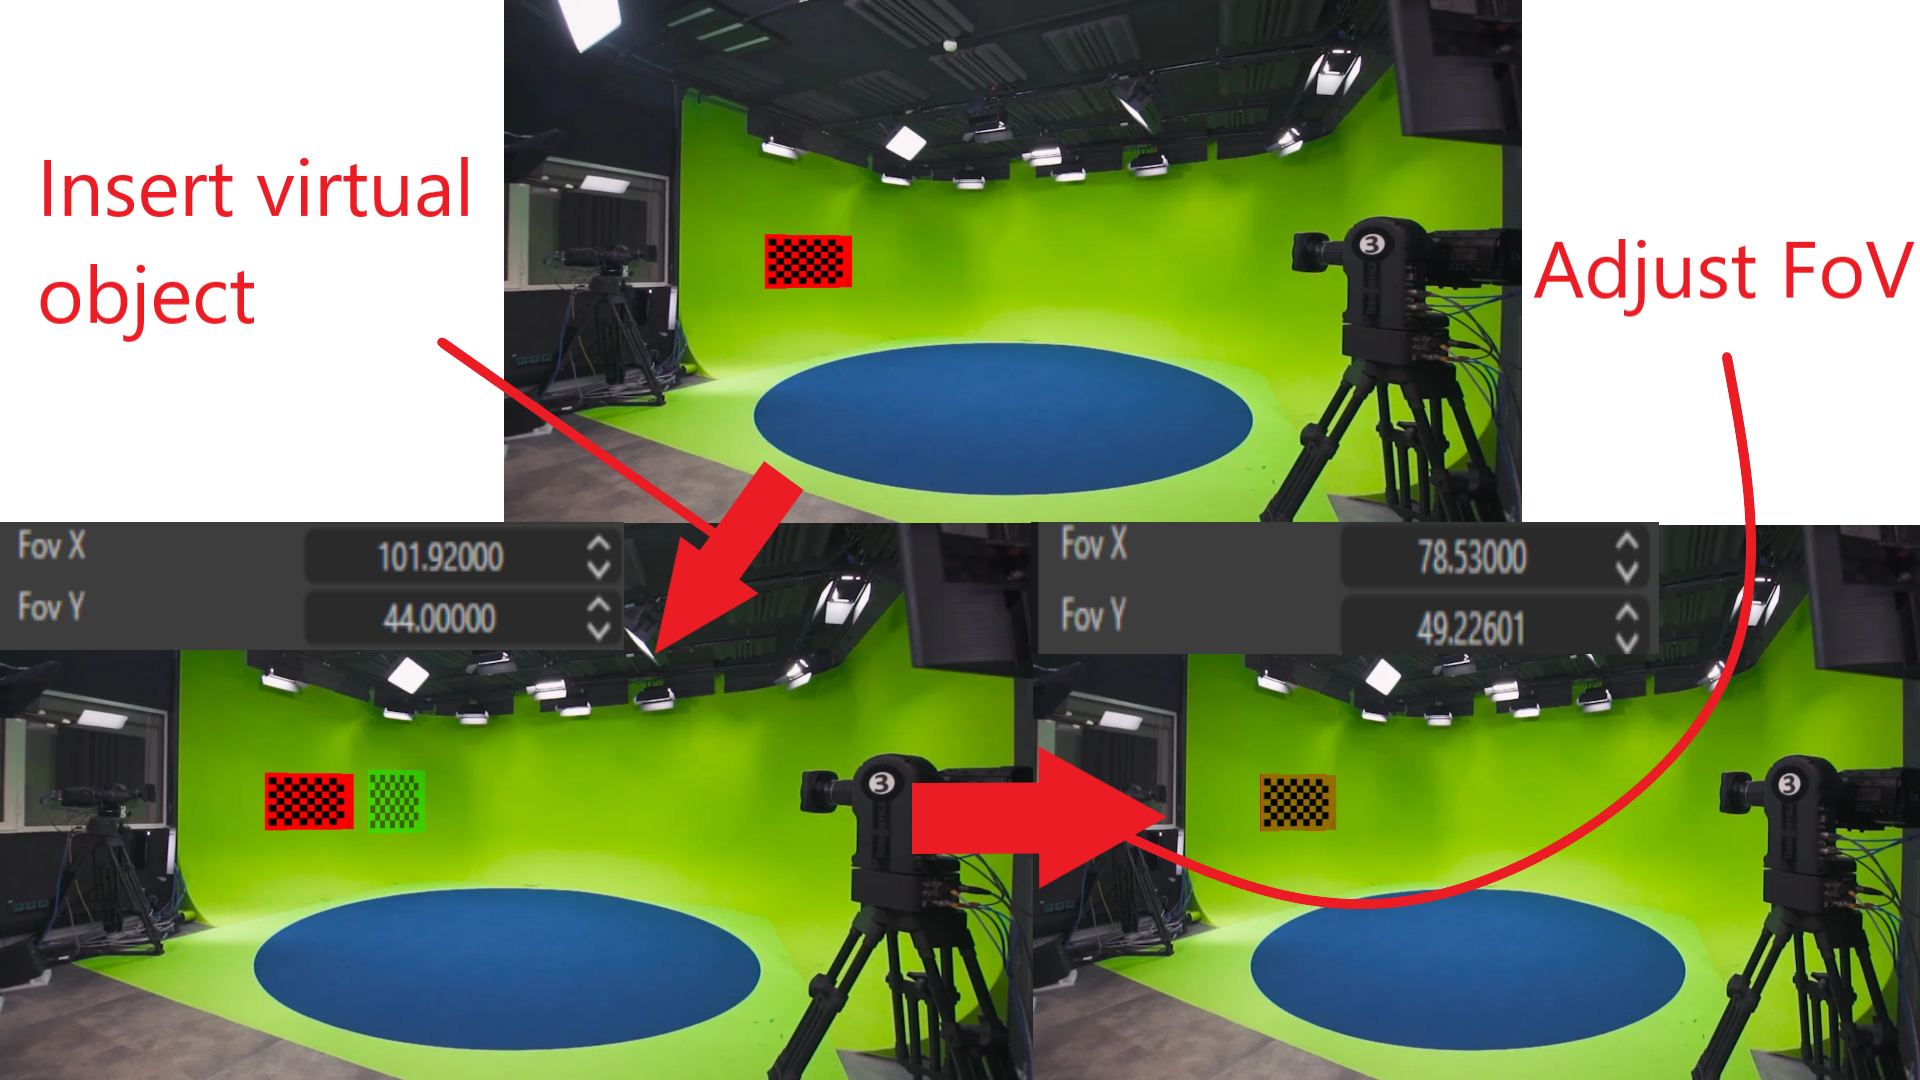
\includegraphics[width=\textwidth]{Images/01intro/FoV_procedure.png}
    \caption{FoV calibration procedure example}
    \label{fig:FoV_pro}
    \end{figure}

    \item \textbf{\( k_1 \) and \( k_2 \):} Move the object to the edges of the frame. Adjust \( k_1 \) and \( k_2 \) coefficients until alignment is achieved. Repeat across all zoom levels. Figure \ref{fig:K1_pro} illustrates the K1 calibration. The K2 calibration is analog to the K1 calibration, however the real object should be moved to the corner of the image. Figure \ref{fig:CP} illustrates where the object needs to be for each specific coefficient calibration.

    \begin{figure}[h]
    \centering
    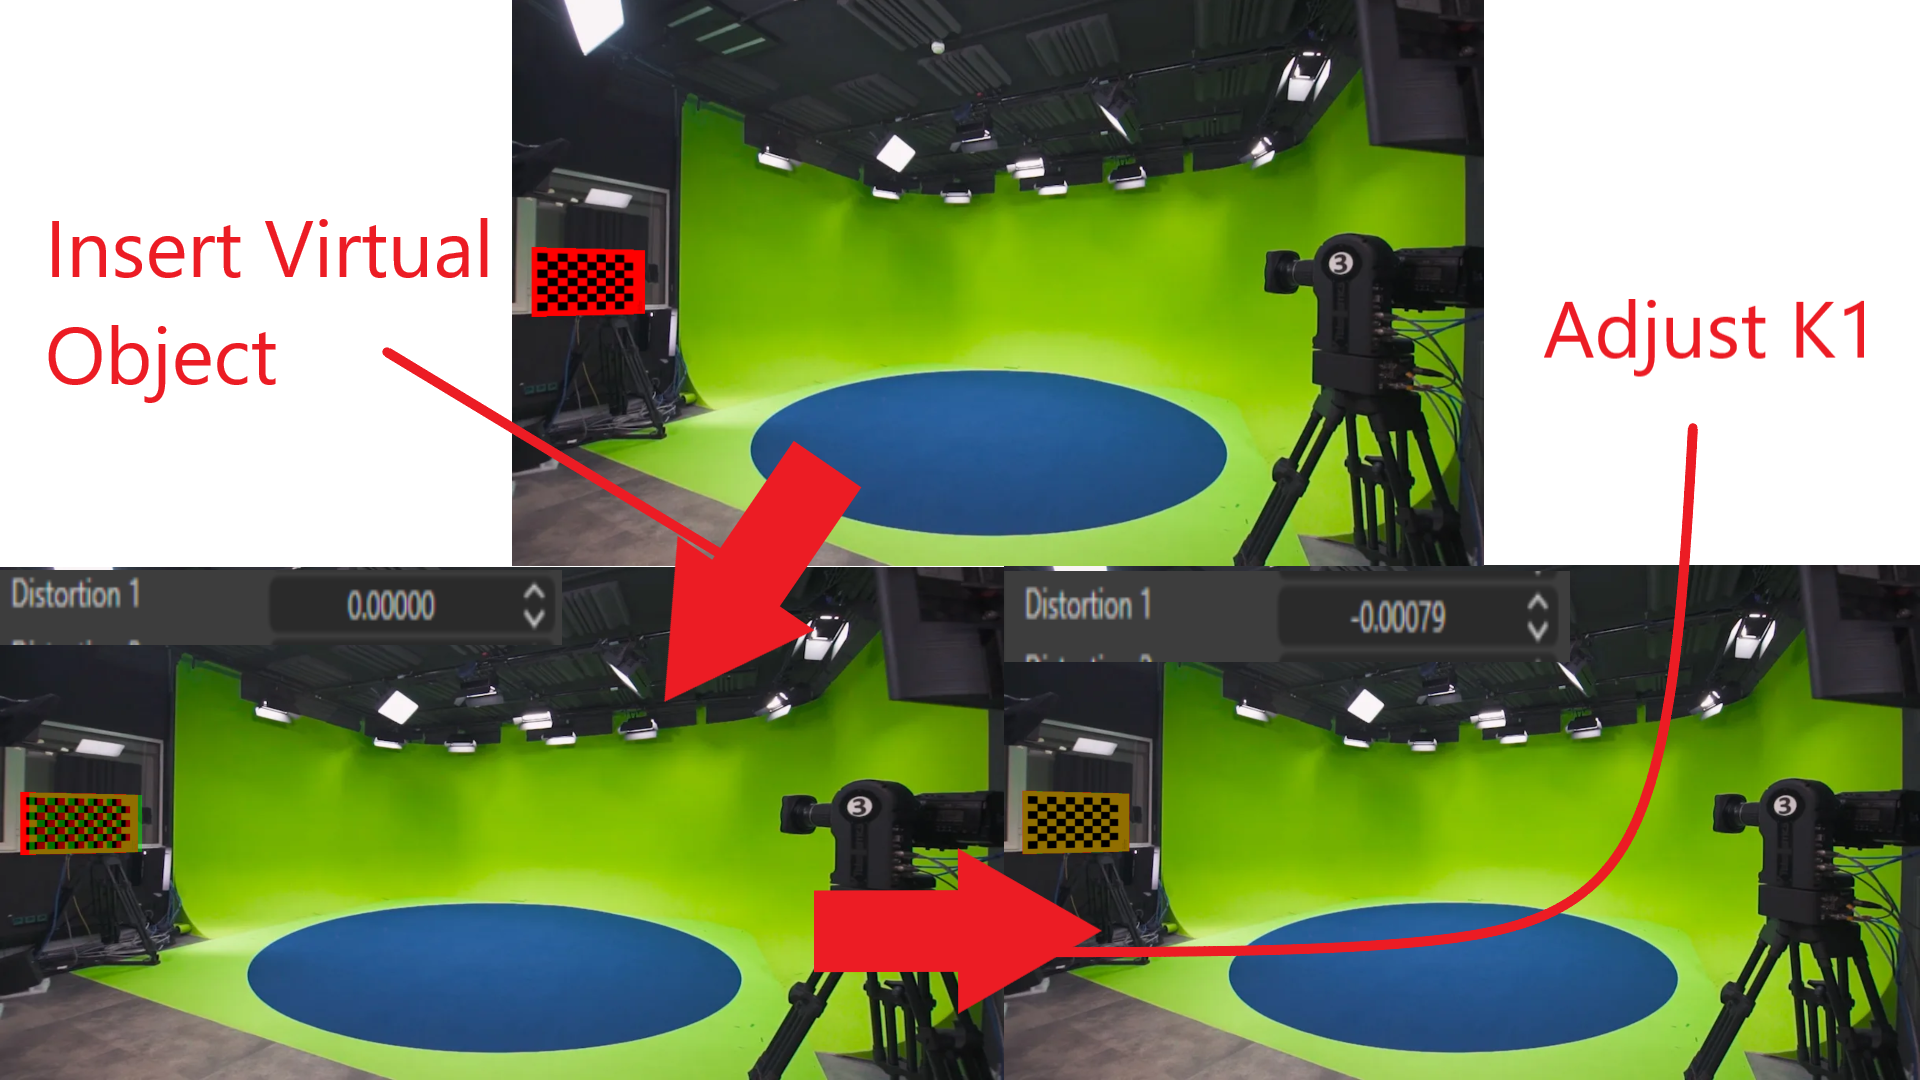
\includegraphics[width=\textwidth]{Images/01intro/K1_pro.png}
    \caption{K1 calibration procedure example}
    \label{fig:K1_pro}
    \end{figure}
    
    \item \textbf{Nodal Point:} Follow the steps to align two reference objects at different depths, ensuring there is \textbf{no parallax effect}\footnote{The \textbf{no parallax effect} occurs when a camera rotates around its \textit{nodal point}, preventing any apparent shift between foreground and background objects. This ensures that elements at different depths remain perfectly aligned, eliminating unwanted distortions caused by parallax. Achieving this effect is crucial for seamless panoramic photography and precise image stitching, as it allows multiple frames to blend naturally without misalignment.} when the camera rotates slightly.
\end{enumerate}


\noindent Figure \ref{fig:CP} represents the location where the real object should be for each coefficient determination.

\begin{figure}
    \centering
    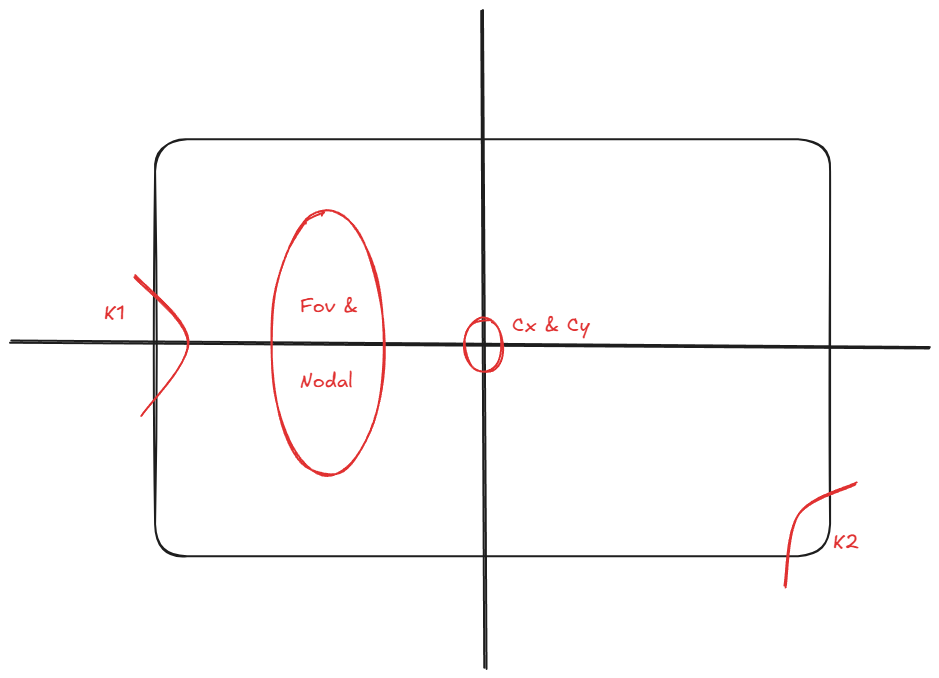
\includegraphics[width=\textwidth]{Images/02stateart/Calibration Parameters.png}
    \caption{Calibration Parameters}
    \label{fig:CP}
\end{figure}

\subsubsection*{Challenges of Current Method}

\noindent The current solution is effective, but it has limitations:

\begin{itemize}
    \item Time-intensive calibration process.
    

    \begin{table}[h]
        \centering
        \begin{tabular}{|l|c|}
            \hline
            \textbf{Coefficient} & \textbf{Calibration Time (min)} \\ \hline
            Center-shift & 5 - 10 \\ \hline
            FoV & 60 - 120 \\ \hline
            K1 & 60 - 120 \\ \hline
            K2 & 60 - 120 \\ \hline
            Nodal & 60 - 120 \\ \hline
        \end{tabular}
        \caption{Calibration Times for Each Coefficient}
        \label{tab:calibration_times}
    \end{table}

    \item Reliance on operator expertise for accurate results.
    \item Lack of automation for dynamic zoom and focus adjustments.
\end{itemize}

\subsection{Goals and Metrics}

\noindent The primary goal of this project is to improve the calibration process, making it faster, more reliable, and less dependent on the expertise of the operator. The success of this solution will be evaluated based on:

\begin{enumerate}
    \item \textbf{Accuracy of the distortion coefficients compared to manual calibration.} This accurancy will me measured by simulating images with known distortion coefficients using the $R^3$ software and comparing them to the experimental results. The goal is for each coefficient to have a relative error of less then 5\%.
    \item \textbf{Reduction in calibration time.} The goal is to reduce the calibration time to 30 minutes or less.
    \item \textbf{Consistency across multiple zoom and focus levels.} Which will be measured by analysing multiple zoom and focus levels and comparing the results.
    \item \textbf{Automation of the calibration process.} The goal is to automate the calibration process as much as possible, reducing the need for manual adjustments.
\end{enumerate}

\section{Document Overview}\label{sec:doc_overview}

\chapter{State of the Art}\label{chap:state_art}

\section{Understanding the Basics}

\noindent Before diving into a detailed explanation, it is essential to understand some foundational concepts. The following sections provide simplified explanations of these key concepts:

\begin{enumerate}
    \item What is \ac{AR} ?
    \item What is lens distortion?
    \item What is the $R^3$ software?
\end{enumerate}

\subsection{What is augmented reality}

\noindent \ac{AR} is a technology that overlays digital information—such as images, sounds, or text—onto the real world. Unlike \ac{VR}, which creates a fully immersive digital environment, \ac{AR} enhances reality by adding interactive, computer-generated elements. For example, in mobile applications or games like Pokémon GO, digital characters appear as if they are part of the physical world when viewed through the device's camera.\ac{AR} is used in various fields, including gaming, retail, education, and training, to enrich the user experience with additional layers of digital content.

\noindent wTVision implements \ac{AR} on video streaming platforms. Figures \ref{fig:AG_4} and \ref{fig:AG4_overlay} show a frame from a video of an \ac{AR} scene developed by wTVision.

\begin{figure}[h]
    \centering
    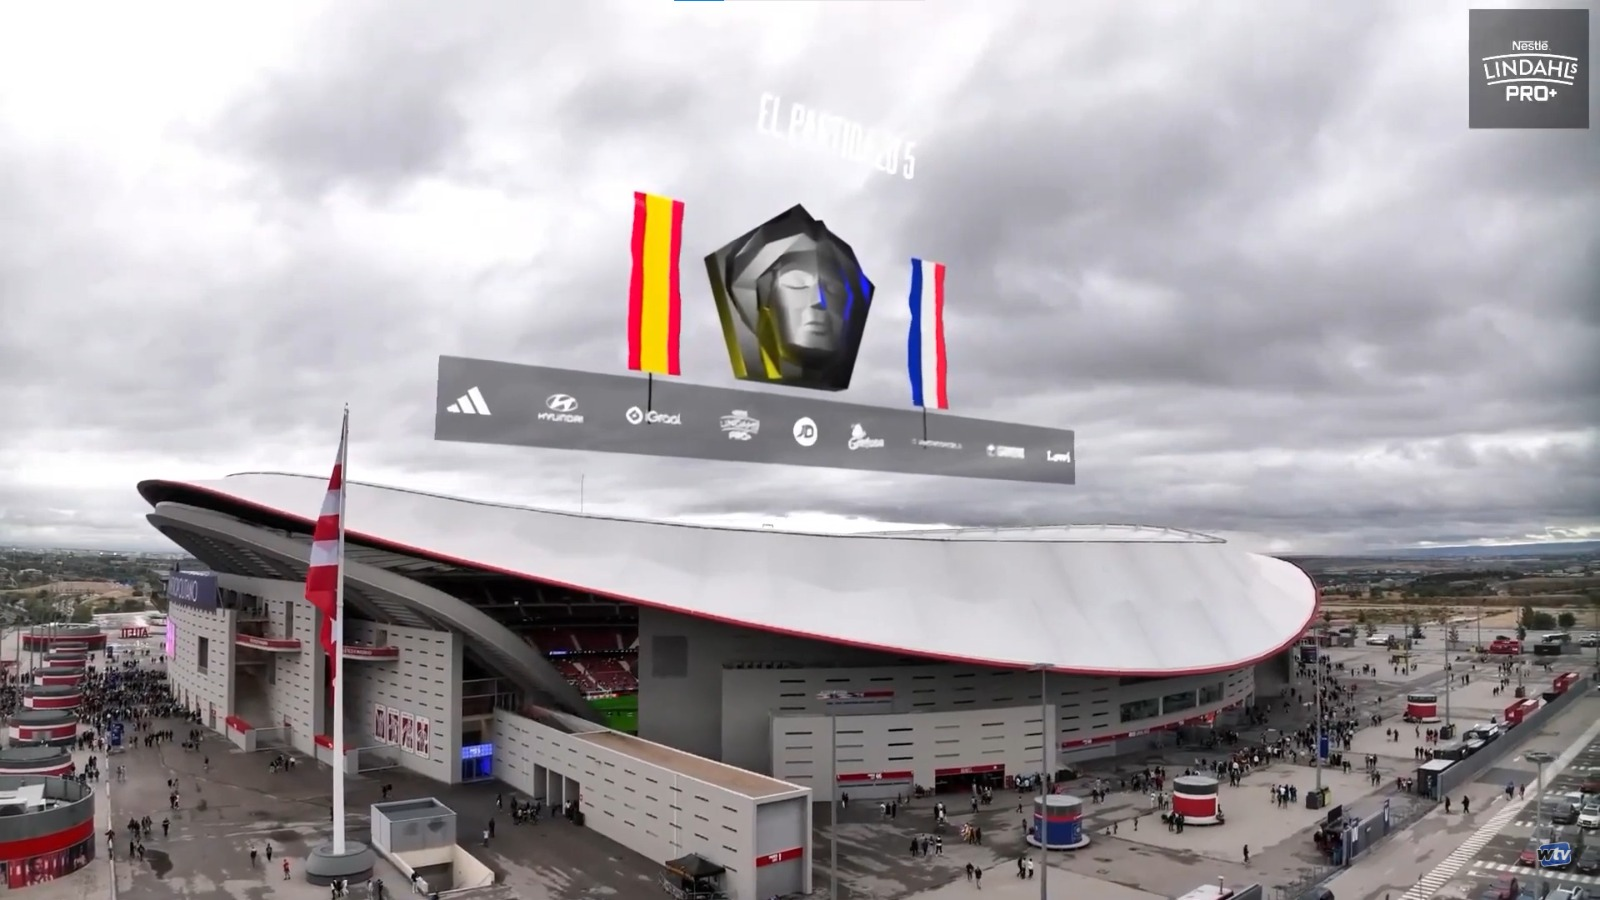
\includegraphics[width=\textwidth]{Images/02stateart/AG_4.jpeg}
    \caption{Example of an \ac{AR} scene developed by wTVision}
    \label{fig:AG_4}
\end{figure}

\begin{figure}[h]
    \centering
    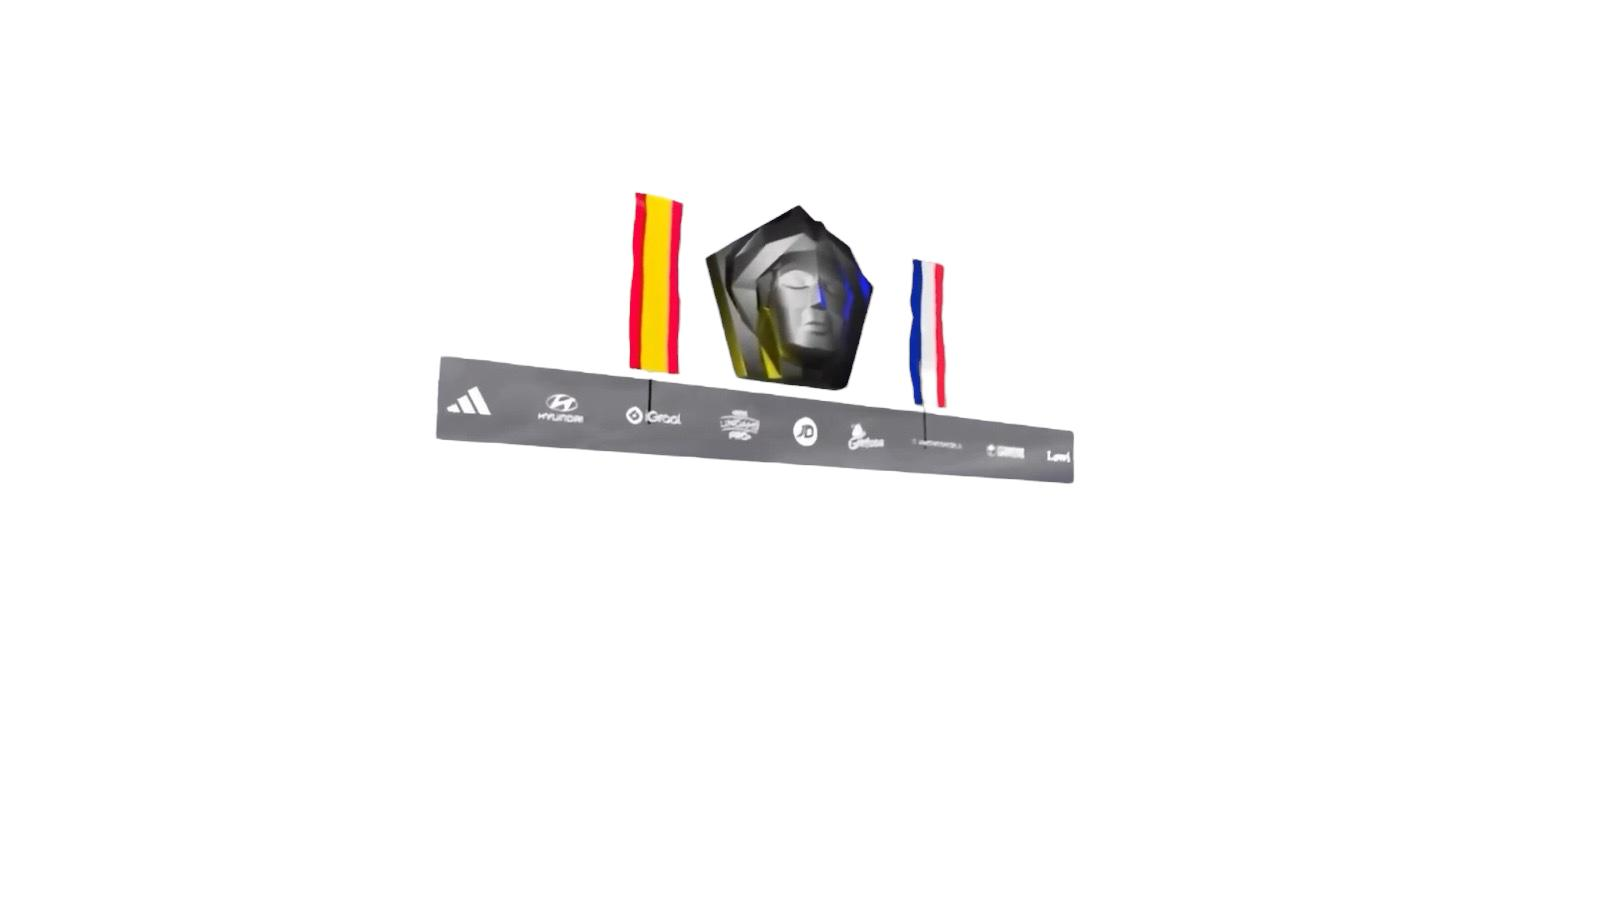
\includegraphics[width=\textwidth]{Images/02stateart/AG_4_overlay.jpeg}
    \caption{Overlay used in the scene shown in Figure \ref{fig:AG_4}}
    \label{fig:AG4_overlay}
\end{figure}

\subsection{What is Lens Distortion}

\noindent Lens distortion is an optical effect in which straight lines appear curved or warped in a photograph, image, or video due to imperfections in the lens shape and due to the physics of optics. This effect commonly occurs with wide-angle and zoom lenses, distorting the real-world perspective and causing objects near the edges of the image to appear stretched or compressed. Figure \ref{fig:lens} illustrates various types of lens distortion.

\begin{figure}[h]
    \centering
    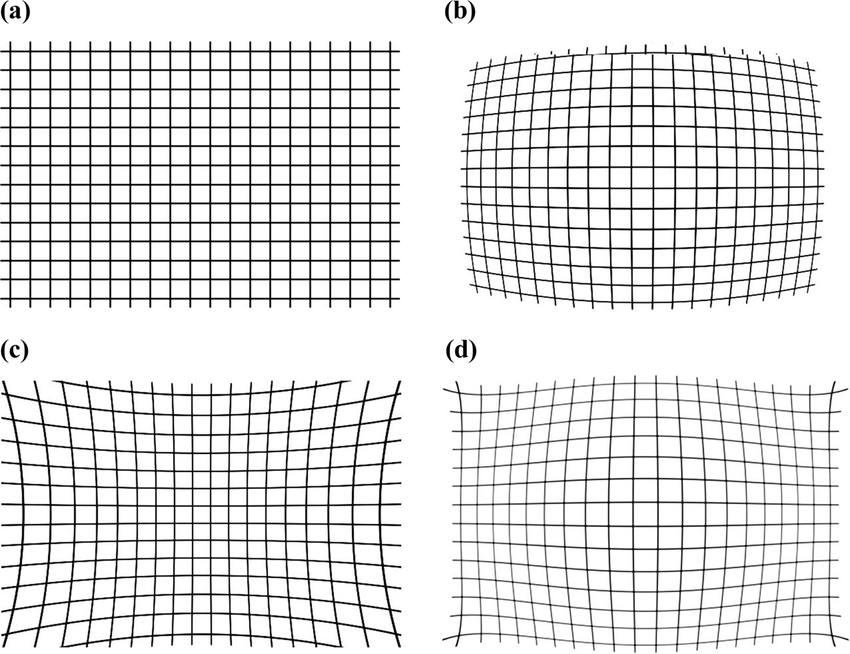
\includegraphics[width=\textwidth]{Images/02stateart/Types-of-lens-distortion-a-Non-distortion-b-Barrel-distortion-c-Pincushion.tif.png}
    \caption{Types of lens distortions: (a) Non-distortion, (b) Barrel distortion, (c) Pincushion distortion, (d) Mixed types of distortion}
    \label{fig:lens}
\end{figure}

\noindent Cameras used by wTVision have some degree of distortion, although it is not very noticeable. However, when inserting virtual overlays in a video, it is crucial to distort the virtual environment in the same way the camera lens distorts the real world. This ensures that virtual objects appear realistic and correctly aligned. Without this distortion, virtual objects would appear out of place when inserted into the real-world scene.

\subsection{What is the $R^3$ Software}

\noindent To address this issue, wTVision developed the $R^3$ software. This tool includes an engine and a software platform that provides the necessary technology to create and render digital environments. Within the platform, the "Space Designer" tool allows developers to build, layout, and arrange the virtual environment where the interactive experience takes place. While the engine handles rendering graphics, processing physics, and managing assets, the Space Designer offers an interactive, visual interface for creating the look and feel of the virtual world. Figure \ref{fig:interface} shows the $R^3$ Space Designer interface.

\begin{figure}[h]
    \centering
    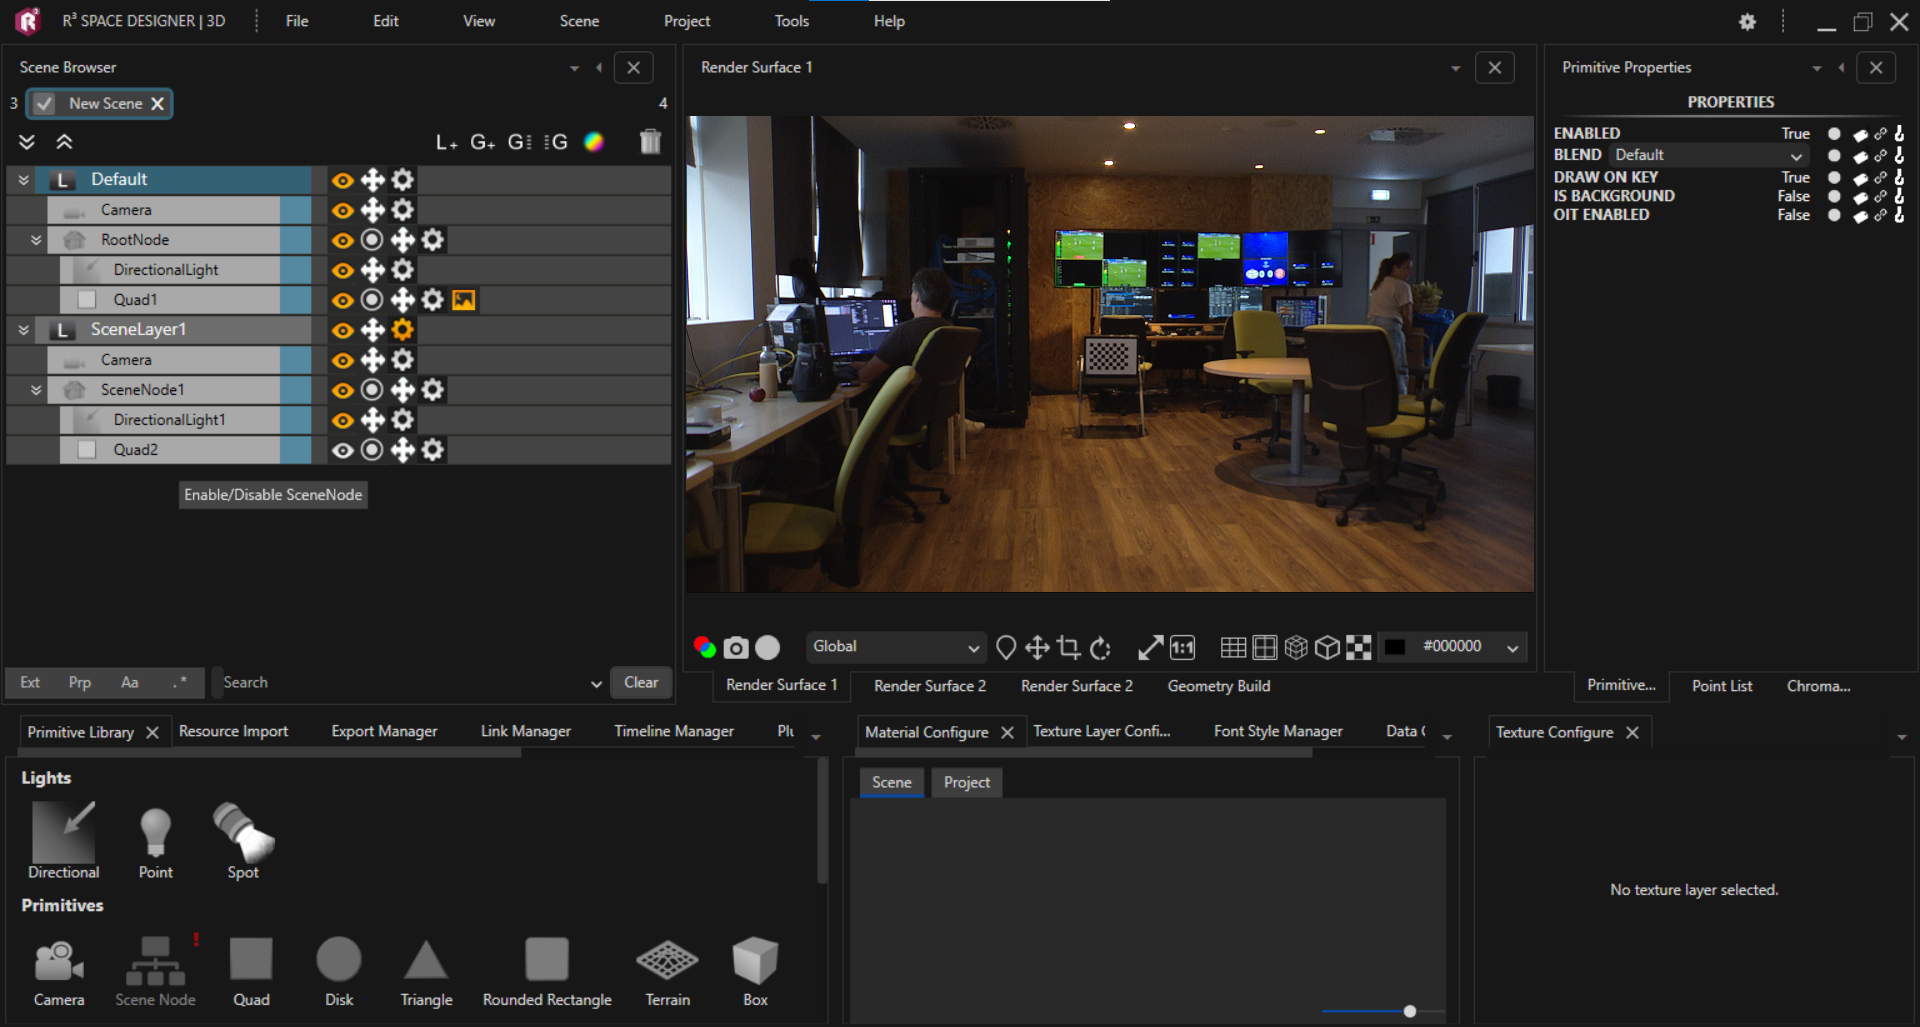
\includegraphics[width=\textwidth]{Images/02stateart/interface.png}
    \caption{$R^3$ Space Designer interface}
    \label{fig:interface}
\end{figure}

\section{Virtual Environment Calibration}

\noindent Earlier, we mentioned that wTVision developed the $R^3$ software to calibrate the virtual environment. This section explains why they developed a specialized tool instead of using existing tools like OpenCV for determining rectification coefficients, and it examines the pros and cons of the software.

\subsection{Common Lens Distortion Problems}

\noindent First, let’s clarify how typical lens distortion issues are handled. For example, photographers using professional cameras frequently encounter distorted images, as shown in Figure \ref{fig:prof_camera}.

\begin{figure}[h]
    \centering
    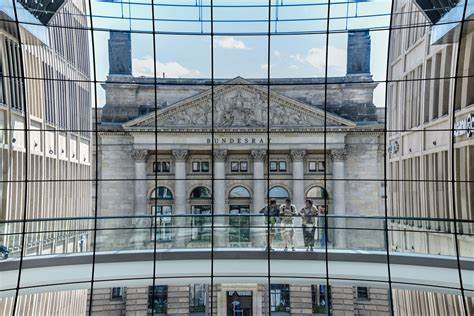
\includegraphics[width=\textwidth]{Images/02stateart/professional camera.png}
    \caption{Example of a distorted image taken with a professional camera}
    \label{fig:prof_camera}
\end{figure}

\noindent To correct these distortions, the OpenCV library is often used by applying specific distortion coefficients.

\noindent The main types of lens distortion are \textbf{Radial Distortion} and \textbf{Tangential Distortion}. Each type has distinct causes and visual effects, which are explained below.

\subsection{Types of Lens Distortion}

\begin{itemize}
    \item \textbf{Radial Distortion:}
    
    Radial distortion occurs when light rays bend unevenly as they pass through the lens, causing straight lines to appear curved. This distortion is more pronounced at the image edges and is mathematically described by:

    \begin{align}
        x_{\text{distorted}} &= x \left(1 + k_1 r^2 + k_2 r^4 + k_3 r^6\right) \\
        y_{\text{distorted}} &= y \left(1 + k_1 r^2 + k_2 r^4 + k_3 r^6\right)
    \end{align}

    where \( k_1 \), \( k_2 \), and \( k_3 \) are radial distortion coefficients, and \( r \) represents the distance from the optical center.

    \item \textbf{Tangential Distortion:}
    
    Tangential distortion results from misalignment between the camera sensor and the lens, causing image points to shift in a direction based on their position. This distortion is modeled by:

    \begin{align}
        x_{\text{distorted}} &= x + \left[2 p_1 x y + p_2 \left(r^2 + 2 x^2\right)\right] \\
        y_{\text{distorted}} &= y + \left[p_1 \left(r^2 + 2 y^2\right) + 2 p_2 x y\right]
    \end{align}

    where \( p_1 \) and \( p_2 \) are tangential distortion coefficients.
\end{itemize}

\subsection{Correcting Lens Distortion with OpenCV}

\noindent To correct these distortions, OpenCV uses a set of distortion coefficients. The five main coefficients—\( k_1 \), \( k_2 \), \( p_1 \), \( p_2 \), and \( k_3 \)—capture both radial and tangential distortion effects:

\begin{equation}
    \text{Distortion Coefficients} = \left(\begin{array}{lllll}
        k_1 & k_2 & p_1 & p_2 & k_3
    \end{array}\right)
\end{equation}

\noindent OpenCV can use these coefficients to rectify distorted images.

\subsection{Challenges in Using OpenCV for Virtual Environment Calibration}

\noindent As mentioned, this project does not aim to rectify images but to calibrate the geometry of a virtual environment. For this, we need to determine the camera's distortion coefficients.

\noindent OpenCV calculates distortion coefficients like \( k_1 \), \( k_2 \), \( p_1 \), \( p_2 \), and \( k_3 \) to correct image distortion. However, for our specific needs, additional coefficients are required that OpenCV cannot provide:

\begin{itemize}
    \item \textbf{Central-Shift:} Due to misaligned lenses, the real-world origin point (0,0,0) and the virtual one may differ, necessitating a central-shift coefficient.
    \item \textbf{No Parallax Effect Coefficient:} To achieve the No Parallax Effect, the virtual environment must behave similarly to the camera, with minimized parallax. The No Parallax Effect coefficient aims to eliminate the apparent shift in object positions due to a viewpoint change. Figure \ref{fig:pen} illustrates this phenomenon. The first image depicts a person's view with both eyes open, offering a complete perspective of the object. In contrast, the second image illustrates the shift in perspective that occurs when one eye is closed, significantly altering the perception of the object.
    \item \textbf{Field of View (FoV):} The \textbf{field of view (FOV)} is the extent of the scene captured by the camera, measured in degrees. It depends on the focal length and sensor size, with wider angles covering more of the scene and narrower angles focusing on a smaller area. Adjusting the camera's zoom changes the FoV, alters the perceived distance of objects. Replicating this effect in \ac{AR} requires altering the FoV in the virtual environment.
\end{itemize}


\begin{figure}
    \centering
    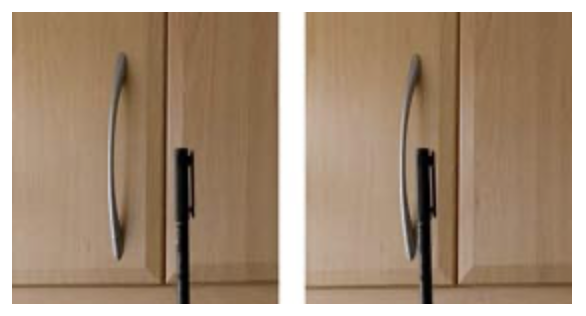
\includegraphics[width=\textwidth]{Images/02stateart/pen.png}
    \caption{Parallax Effect with the human eye.Left picture depicts
    a person’s view with both eyes open. Right picture depicts the shift in perspective that occurs when one eye is closed.}
    \label{fig:pen}
\end{figure}

\section{Communication Between Python and \texorpdfstring{$R^3$}{R3}}
\label{sec:communication_python_r3}

\noindent In this work, the communication between Python and the \textit{R\textsuperscript{3}} software is implemented using sockets. Sockets are a fundamental mechanism in computer systems that enable processes to exchange data. While traditionally used for communication over a network, sockets can also be employed to facilitate communication between processes on the same machine, leveraging the system's networking stack for local inter-process communication (IPC) \cite{stevens2003unix, silberschatz2018os}.

\subsection{Why Sockets for Communication}
\noindent Sockets provide a simple and robust interface for connecting applications written in different programming languages. In this case, Python acts as the controlling script, orchestrating the execution of the \textit{R\textsuperscript{3}} software. Using sockets offers the following advantages:
\begin{itemize}
    \item \textbf{Language Agnosticism:} Python and \textit{R\textsuperscript{3}} operate independently, and sockets enable communication without requiring language-specific bindings or modifications to the software \cite{beejGuide, pythonDocsSocket}.
    \item \textbf{Asynchronous Communication:} Sockets allow Python to send commands to \textit{R\textsuperscript{3}} and wait to receive responses at different rates, enabling efficient two-way communication \cite{stevens2003unix}.
    \item \textbf{Local Communication:} Although sockets are often associated with network communication, they can be used for local IPC by binding the socket to the loopback interface (localhost). This ensures that all communication remains within the same machine, minimizing latency and security concerns \cite{silberschatz2018os}.
\end{itemize}

\subsection{Implementation Overview}
\noindent The implementation of the communication relies on a server-client model \cite{beejGuide}:
\begin{enumerate}
    \item \textbf{Socket Initialization:} A socket initialized in Python connection it to the $R^3$ software, configured as the server, and bound to a specific port (9009) on the loopback address (127.0.0.1) \cite{pythonDocsSocket}.
    \item \textbf{Connection from \textit{R\textsuperscript{3}}:} Python acts as a client, connecting to $R^3$.
    \item \textbf{Message Exchange:} Once connected, Python sends commands or data to \textit{R\textsuperscript{3}}, and the latter processes the instructions and responds via the same socket \cite{stevens2003unix}.
    \item \textbf{Closing the Connection:} After the data exchange is complete, the connection is gracefully closed, releasing resources.
\end{enumerate}

\subsection{Commands for Interaction with the Engine}
\label{subsec:engine_commands}

\noindent The communication between Python and the \textit{R\textsuperscript{3}} software, as outlined in Section~\ref{sec:communication_python_r3}, enables the execution of specific commands to interact with the engine's functionality. Below, we describe the key commands used in this implementation, their purposes, and their syntax, as demonstrated in the provided examples.

\subsubsection{Basic Engine Interaction Commands}
\begin{itemize}
    \item \textbf{TakeSnapshot:} This command captures a snapshot of the render surface and saves it as a PNG image. The default save location is the "Projects" folder, but users can specify a custom path and filename. The command supports two syntaxes:
    \begin{itemize}
        \item \texttt{engine.takeSnapshot "file\_name"}: Saves the snapshot with the specified filename in the default "Projects" folder.
        \item \texttt{engine.takeSnapshot "path\_with\_filename"}: Saves the snapshot at the specified path with the given filename.
    \end{itemize}
    Upon success, the engine responds with \texttt{"OK: SNAPSHOT TAKEN"}. If an invalid path is provided, it returns an error message: \texttt{"ERROR: SNAPSHOT - INVALID PATH"}. For example:
    \begin{verbatim}
    engine.takeSnapshot "JornalNoiteTicker"
    \end{verbatim}
    saves a snapshot named "JornalNoiteTicker.png" in the default location, while:
    \begin{verbatim}
    engine.takeSnapshot "C:/Users/john.doe/Desktop/JornalNoiteTicker"
    \end{verbatim}
    saves it to a specific desktop path.

    \item \textbf{GetSnapshot:} This command retrieves a snapshot previously taken with \texttt{TakeSnapshot} and returns it as a base64-encoded string. It is essential to use \texttt{TakeSnapshot} before invoking \texttt{GetSnapshot}, as the latter relies on the existence of a snapshot file. The command supports two syntaxes:
    \begin{itemize}
        \item \texttt{engine.getSnapshot "file\_name"}: Retrieves the snapshot with the specified filename from the default "Projects" folder.
        \item \texttt{engine.getSnapshot "path\_with\_filename"}: Retrieves the snapshot from the specified path and filename.
    \end{itemize}
    Upon success, the engine responds with:
    \begin{verbatim}
    "OK: <IMAGE> base64string <IMAGE>"
    \end{verbatim}
    If the snapshot file cannot be found or the path is invalid, it returns an error message, such as:
    \begin{verbatim}
    "ERROR: GETSNAPSHOT - COULD NOT READ LAST SNAPSHOT FILE"
    "ERROR: GETSNAPSHOT - INVALID PATH"
    \end{verbatim}
    For instance:
    \begin{verbatim}
    engine.getSnapshot "JornalNoiteTicker"
    \end{verbatim}
    returns the base64-encoded image data for the snapshot named "JornalNoiteTicker.png" in the default location.

    \item \textbf{Get:} This command retrieves the current tracking packet from a specified tracking camera, providing detailed camera parameters and status. The syntax is:
    \begin{verbatim}
    engine.tracking "tracking_camera_name" get
    \end{verbatim}
    Upon success, the engine responds with:
    \begin{verbatim}
    "OK: CURRENT CAMERA PARAMETERS:"
    \end{verbatim}
    followed by a JSON-like structure containing parameters such as field of view (FovX, FovY), aspect ratio, position (PosX, PosY, PosZ), rotation (RotX, RotY, RotZ), and other metadata like view matrix, center coordinates, and sensor size. For example:
    \begin{verbatim}
    engine.tracking "Cam0" get
    \end{verbatim}
    might return a response detailing the parameters of the "Cam0" tracking camera, including:
    \begin{verbatim}
    "FovX": 80.0, "FovY": 50.0, ...
    \end{verbatim}
\end{itemize}

\subsubsection{Scene Export Commands}
\noindent In addition to the basic engine interaction commands, the system supports a set of more complex \textit{Scene Export} commands for managing and manipulating scene properties within \textit{R\textsuperscript{3}}. These commands operate on export entities (e.g., properties like transform positions, scales, or text values) and can be executed individually or in batches (via \textit{MultiExport}). Below, we detail each command and its functionality:

\begin{itemize}
    \item \textbf{SetValue:} This command sets the value of a specific export property within a scene. The syntax is:
    \begin{verbatim}
    scene "project_ref/scene_ref" export "export_name" SetValue "value"
    \end{verbatim}
    \item \textbf{Rename:} This command renames an existing export within a scene. The syntax is:
    \begin{verbatim}
    scene "project_ref/scene_ref" export "export_name" rename "new_name"
    \end{verbatim}
    \item \textbf{GetValue:} This command retrieves the current value of a specific export property within a scene. The syntax is:
    \begin{verbatim}
    scene "project_ref/scene_ref" export "export_name" getValue
    \end{verbatim}
    \item \textbf{MultiExport Commands:} These commands allow batch operations on multiple exports. Example:
    \begin{verbatim}
    scene "JornalNoite/teste" export "transform.scale" SetValue "1,2,1"
          "text" SetValue "player_name" "alpha" SetValue "0.5"
    \end{verbatim}
    returns:
    \begin{verbatim}
    "OK: SCENE EXPORT SETVALUE - Value Set."
    "OK: SCENE EXPORT SETVALUE - Value Set."
    "OK: SCENE EXPORT SETVALUE - Value Set."
    \end{verbatim}
\end{itemize}

\noindent These \textit{Scene Export} commands provide fine-grained control and automation through Python scripts, enabling efficient real-time scene manipulation.


\subsection{Benefits of Local Socket Communication}
\noindent By utilizing sockets for communication between Python and \textit{R\textsuperscript{3}}, this setup ensures modularity and scalability. Python and \textit{R\textsuperscript{3}} remain decoupled, allowing for independent updates or replacements of either component without affecting the communication protocol. Additionally, the use of the loopback interface ensures that no external networking hardware or configuration is required \cite{silberschatz2018os}.

\subsection{Applications and Future Potential}
\noindent This socket-based architecture facilitates a variety of use cases, such as:
\begin{itemize}
    \item Automating tasks in \textit{R\textsuperscript{3}} through Python scripts.
    \item Integrating Python's data analysis and visualization capabilities with \textit{R\textsuperscript{3}}'s functionality.
    \item Enabling real-time monitoring and feedback loops between Python and \textit{R\textsuperscript{3}}.
\end{itemize}

\noindent In summary, the use of sockets for communication between Python and \textit{R\textsuperscript{3}} provides a flexible and efficient solution for inter-process communication, paving the first step to automate the lens calibration.




\chapter{Edge Detection Using OpenCV} \label{chap:Edge Detection Using OpenCV}

The internship project began with the final objective of automating the \ac{AR} camera lens calibration. For that, the following tasks were outlined:
\begin{enumerate}
    \item Develop a program that detects the coordinates (in pixels) of the corners of a quadrilateral target, as well as the corresponding centroid.
    \item Using the centroid coordinates, calibrate the central-shift.
    \item Using the coordinates of the corners of the target, calibrate the FoV and \( k_1 \)/\( k_2 \) coefficients.
    \item Calibrate the nodal point.
\end{enumerate}

The objective is to recreate the calibration procedure that an operator uses. The following sections explain in detail how each task is completed, as well as the limitations and advantages of the current methods.



\section{Canny Edge Detection}
Even though OpenCV cannot directly provide the coefficients required, this library still proves useful for its powerful image object detection functions. 

\noindent Canny edge detection is a multi-step algorithm designed to detect a wide range of edges in images. It begins with noise reduction—typically using a Gaussian filter—to smooth the image and minimize the impact of noise. Next, the algorithm computes the intensity gradients to identify areas with rapid intensity changes, which serve as potential edge locations. To refine these candidate edges, non-maximum suppression is applied to thin the detected edges, ensuring that only the strongest responses are retained. Finally, double thresholding and edge tracking by hysteresis are used to classify edges as strong or weak, and to connect weak edges that are likely part of the same boundary structure \cite{opencv_canny, geeksforgeeks_canny}. An example of Canny's capabilities is shown in figure \ref{fig:pumpkin}.
\begin{figure}[h]
    \centering
    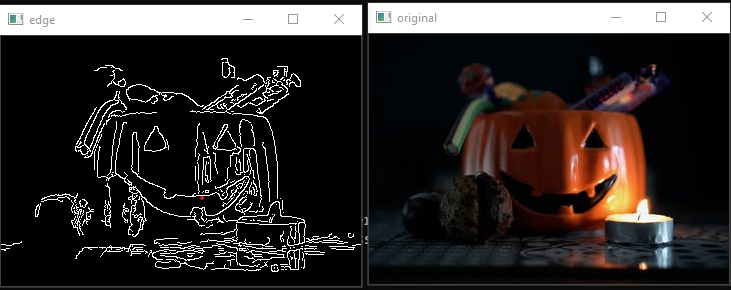
\includegraphics[width=\textwidth]{Images/03edgedetect/pumpkin.png}
    \caption{Example of a canny edge detection application \cite{geeksforgeeks_canny}}
    \label{fig:pumpkin}
\end{figure}


\noindent In the context of this project, the Canny edge detection algorithm is employed to automatically identify the boundaries of a quadrilateral target by using the OpenCV contour approximation functions \cite{contour_approximation, contour}. By accurately detecting the corners and the centroid of the target, the algorithm provides the critical coordinates necessary for calibrating the AR camera lens. These coordinates form the basis for subsequent calibration steps such as central-shift correction, Field of View (FoV) adjustments, and compensation for lens distortion coefficients. The robustness of the Canny method against varying lighting conditions and noise makes it particularly effective for this application.

\noindent For more detailed explanations on the workings and implementation of the Canny edge detection algorithm in Python using OpenCV, readers are encouraged to consult the OpenCV tutorial \cite{opencv_canny} and the GeeksforGeeks guide \cite{geeksforgeeks_canny}. These resources provide insights into the algorithm's multi-stage process and practical considerations in real-world applications.

\noindent The edge detection capabilities of OpenCV were used to 
provide the results shown in Figure \ref{fig:corners}.

\begin{figure}[h]
    \centering
    \includegraphics[width=\textwidth]{Images/02stateart/br1.png}
    \caption{Image taken with the camera with the target at the center}
    \label{fig:target}
\end{figure}

\begin{figure}[h]
    \centering
    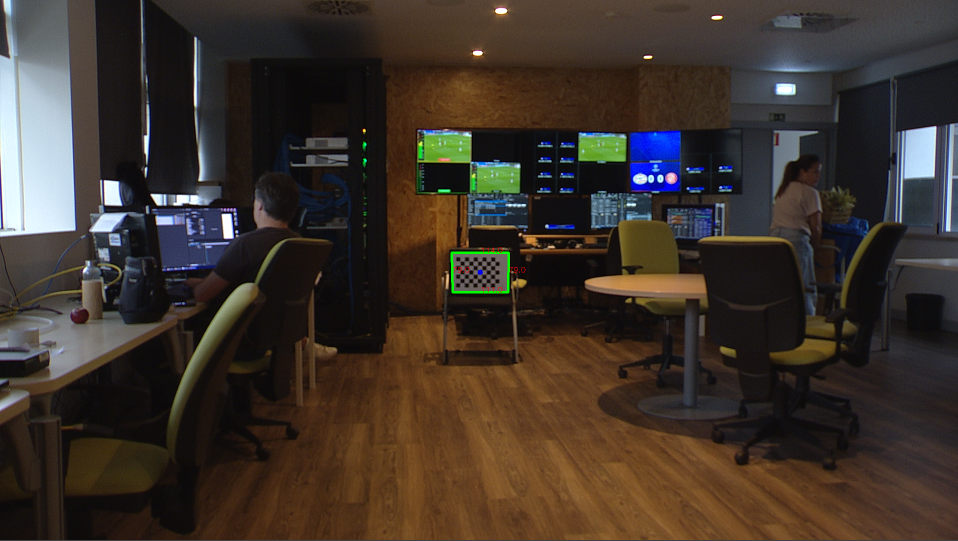
\includegraphics[width=\textwidth]{Images/02stateart/edge_detection.png}
    \caption{Edge detection program demonstration}
    \label{fig:corners}
\end{figure}

\noindent This program enables the detection of the coordinates of the corners and the center of the target, as well as determining the length and width dimensions of the target.

\noindent In conclusion, this section has described the role of Canny edge 
detection in the project, 
emphasizing its utility in identifying the quadrilateral target's corners and centroid. 
The effective detection of these key points supports the calibration process, leading to 
more accurate adjustments in central-shift, FoV, and lens distortion parameters.

\section{Using Blender for Testing}
\label{sec:blender_workflow}
\noindent To evaluate the effectiveness of this program, multiple images from different angles and levels of distortion were needed. However, since the camera is not always available for this project, another program called "Blender" was used to simulate images that would resemble those provided by the real camera. Blender is a free and open-source 3D computer graphics software widely used for creating 3D models, animations, visual effects, and more. In this case, Blender was used to create a virtual camera and virtual targets.

\noindent This section outlines the workflow for setting up and rendering a scene in Blender, a widely used open-source 3D modeling and animation software. The following steps detail how to navigate the interface, adjust objects and camera settings, and produce a rendered image, as applied in this study. Blender was used in this project for simulating images for testing.

\begin{enumerate}
    \item \textbf{Loading a Scene}: Launch Blender and load the desired scene file to begin working with the 3D environment like in figure \ref{fig:load}.
    \begin{figure}[h]
        \centering
        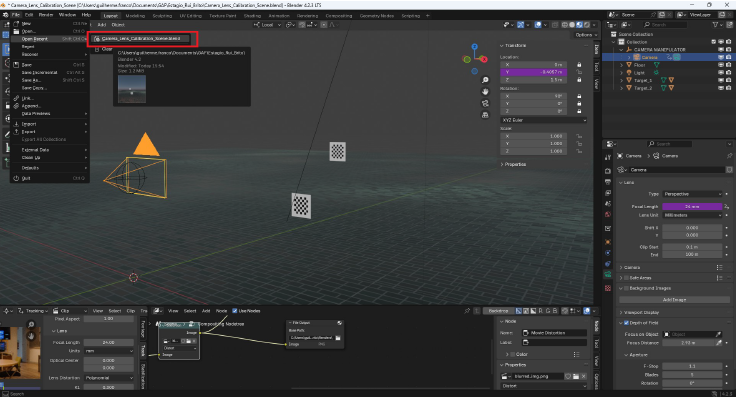
\includegraphics[width=\textwidth]{Images/03edgedetect/1.png}
        \caption{Loading a Scene}
        \label{fig:load}
    \end{figure}

    \item \textbf{Viewport Navigation}: To explore the scene in the Viewport:
    \begin{itemize}
        \item Drag the middle mouse button (MMB) to rotate the view.
        \item Hold Shift and drag MMB to pan across the scene.
        \item Use the mouse wheel to zoom in or out.
    \end{itemize}
    
    \item \textbf{Adjusting Object Positions}: Select the target object (e.g., \texttt{Target\_1} or \texttt{Target\_2}) from the right-hand menu. Modify its position and orientation by:
    \begin{itemize}
        \item Dragging the left mouse button (LMB) on the \textit{Location} and \textit{Rotation} fields.
        \item Typing specific values directly.
        \item Using the interface arrows for incremental adjustments.
    \end{itemize}

    Figure \ref{fig:adjust} illustrates this procedure.

    \begin{figure}[h]
        \centering
        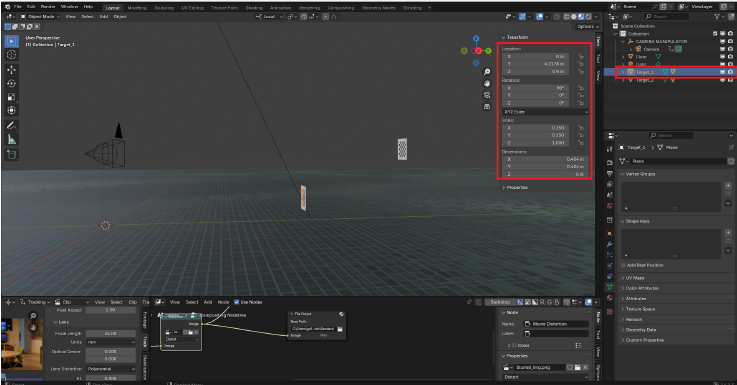
\includegraphics[width=\textwidth]{Images/03edgedetect/2.png}
        \caption{Adjusting Object Positions}
        \label{fig:adjust}
    \end{figure}

    \item \textbf{Aligning the Viewport to the Camera}: To preview the camera’s perspective, press \texttt{Numpad-0} (the zero key on the numeric keypad).
    
    \item \textbf{Camera Positioning}: Select the \texttt{CAMERA\_MANIPULATOR} object and adjust its \textit{Location} and \textit{Rotation} parameters, following the same method as for target objects.
    \begin{figure}[h]
        \centering
        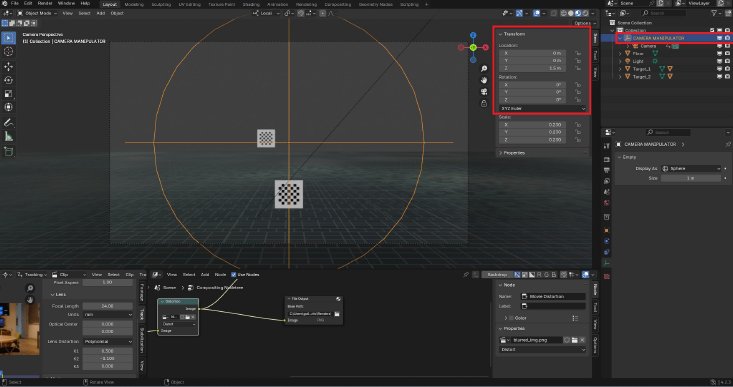
\includegraphics[width=\textwidth]{Images/03edgedetect/3.png}
        \caption{Camera Positioning}
    \end{figure}
    \item \textbf{Camera Lens Settings}: Select the child object \texttt{Camera} under \texttt{CAMERA\_MANIPULATOR}, then access the \textit{Data} sub-menu (indicated by a green camera icon in the bottom-right panel), figure \ref{fig:setting}. Adjust the following:
    \begin{itemize}
        \item \textit{Shift X / Shift Y}: Modify the center shift in the X and Y directions.
        \item \textit{Focus Distance}: Set the camera’s focus point.
        \item \textit{F-Stop}: Control depth of field; lower values increase blur for objects outside the focus distance, while higher values extend the in-focus range.
        \item \textit{Focal Length}: Adjust this parameter (bottom-left corner) to change the field of view (FoV), reflected on the right-hand side.
        \item \textit{K1 and K2}: Edit distortion coefficients directly below the \textit{Focal Length}.
        \item \textit{Nodal Offset}: Represented by the Y-value in the \textit{Location} parameter (displayed in purple). Right-click and select \textit{Edit Driver} to modify its governing function.
    \end{itemize}
    \begin{figure}[h]
        \centering
        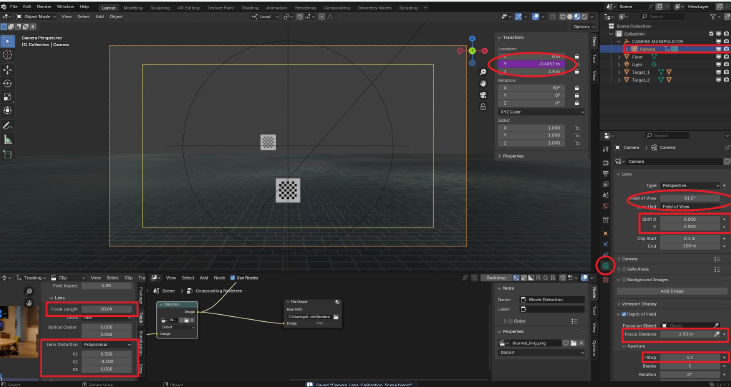
\includegraphics[width=\textwidth]{Images/03edgedetect/4.png}
        \caption{Camera Lens Settings}
        \label{fig:setting}
    \end{figure}
    \item \textbf{Rendering the Image}: From the top-left menu, select \textit{Render $\rightarrow$ Render Image} to initiate the rendering process, figure \ref{fig:render}.
    \begin{figure}[h]
        \centering
        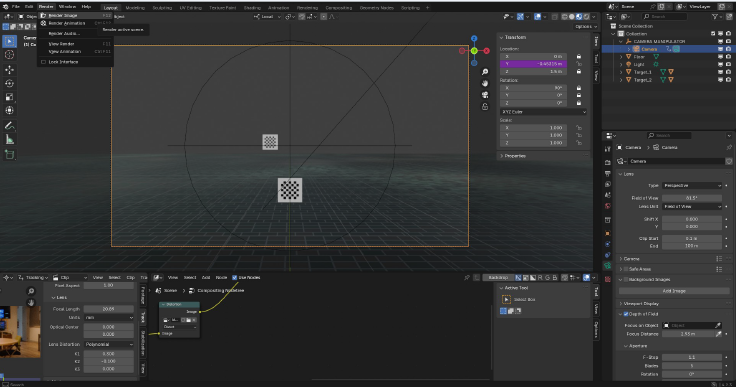
\includegraphics[width=\textwidth]{Images/03edgedetect/5.png}
        \caption{Rendering the Image}
        \label{fig:render}
    \end{figure}
    \item \textbf{Saving the Render}: In the rendering window, wait for the sample calculations to complete, then choose \textit{Image $\rightarrow$ Save As...} to save the output, figure \ref{fig:save}.
    \begin{figure}[h]
        \centering
        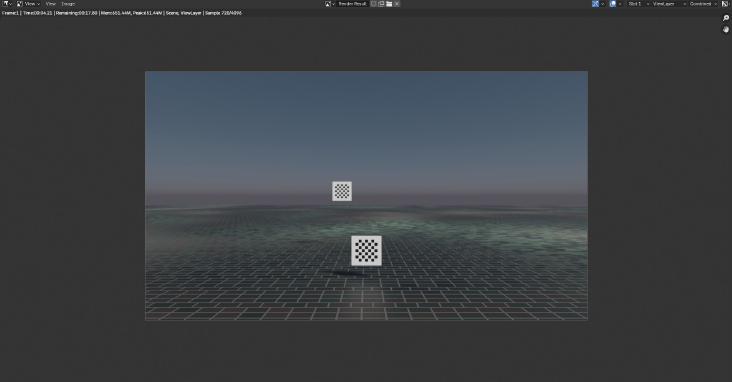
\includegraphics[width=\textwidth]{Images/03edgedetect/6.png}
        \caption{Saving the Render}
        \label{fig:save}
    \end{figure}
    
    \item \textbf{Data Collection}: Currently, data extraction from the rendered image is performed manually. Automation of this process is feasible and could be implemented if deemed beneficial for future work.
\end{enumerate}

\noindent This workflow demonstrates Blender’s capability for precise scene manipulation and rendering, making it a valuable tool for 3D visualization in this research.
To test the edge detection program, only one target was used. Multiple pictures from different angles and with varying distortions were taken and tested. Some of the results are shown in Figure \ref{fig:Edge Detection Results Visualization}.

\begin{figure}[h!]
    \centering
    % First row
    \begin{subfigure}[b]{0.45\textwidth}
        \centering
        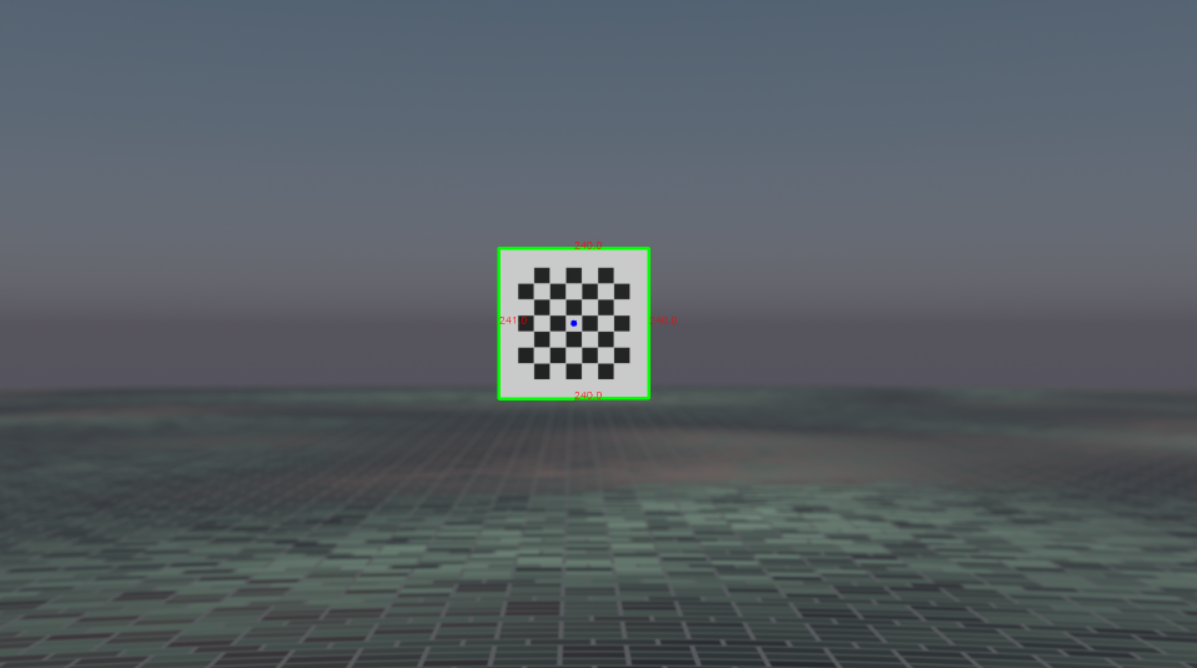
\includegraphics[width=\textwidth]{Images/02stateart/edge_detection_1.png}
        \caption{Image 1}
    \end{subfigure}
    \hfill
    \begin{subfigure}[b]{0.45\textwidth}
        \centering
        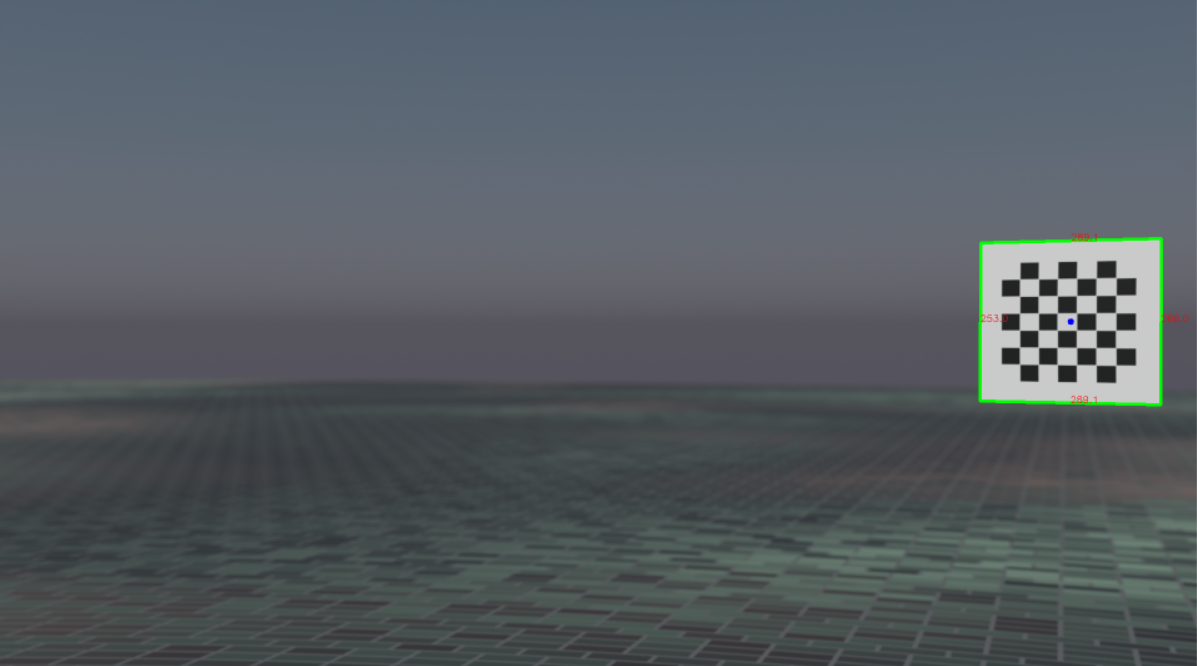
\includegraphics[width=\textwidth]{Images/02stateart/edge_detection_2.png}
        \caption{Image 2}
    \end{subfigure}
    
    \vspace{1cm}
    
    % Second row
    \begin{subfigure}[b]{0.45\textwidth}
        \centering
        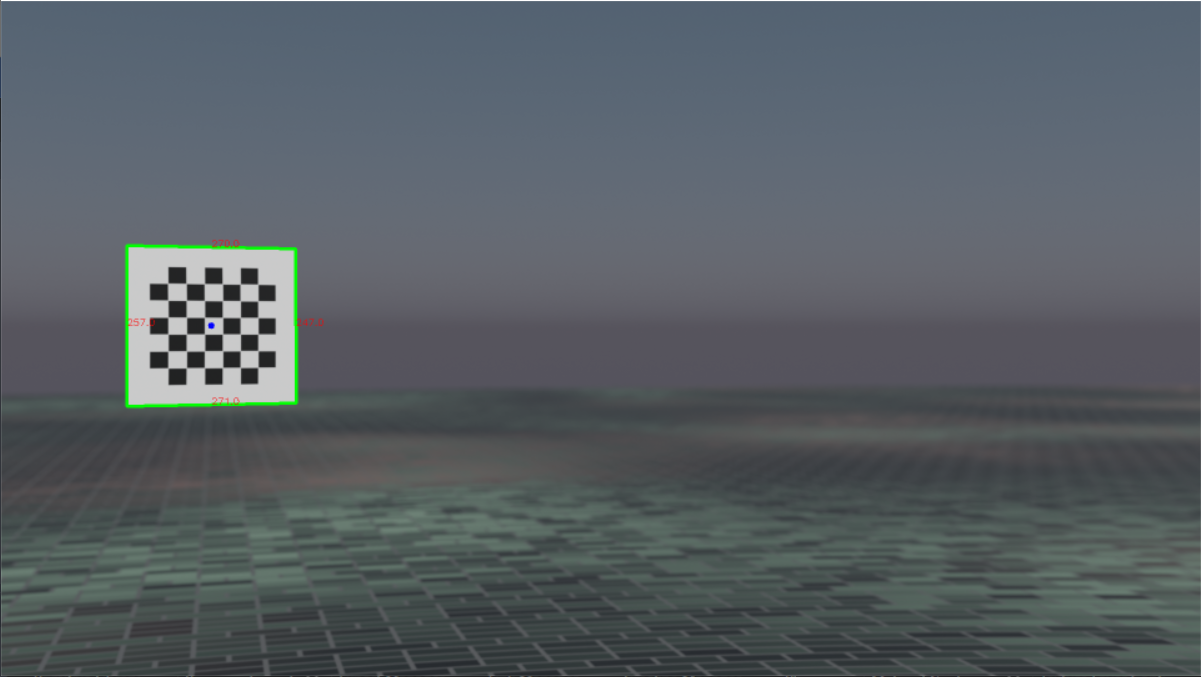
\includegraphics[width=\textwidth]{Images/02stateart/edge_detection_3.png}
        \caption{Image 3}
    \end{subfigure}
    \hfill
    \begin{subfigure}[b]{0.45\textwidth}
        \centering
        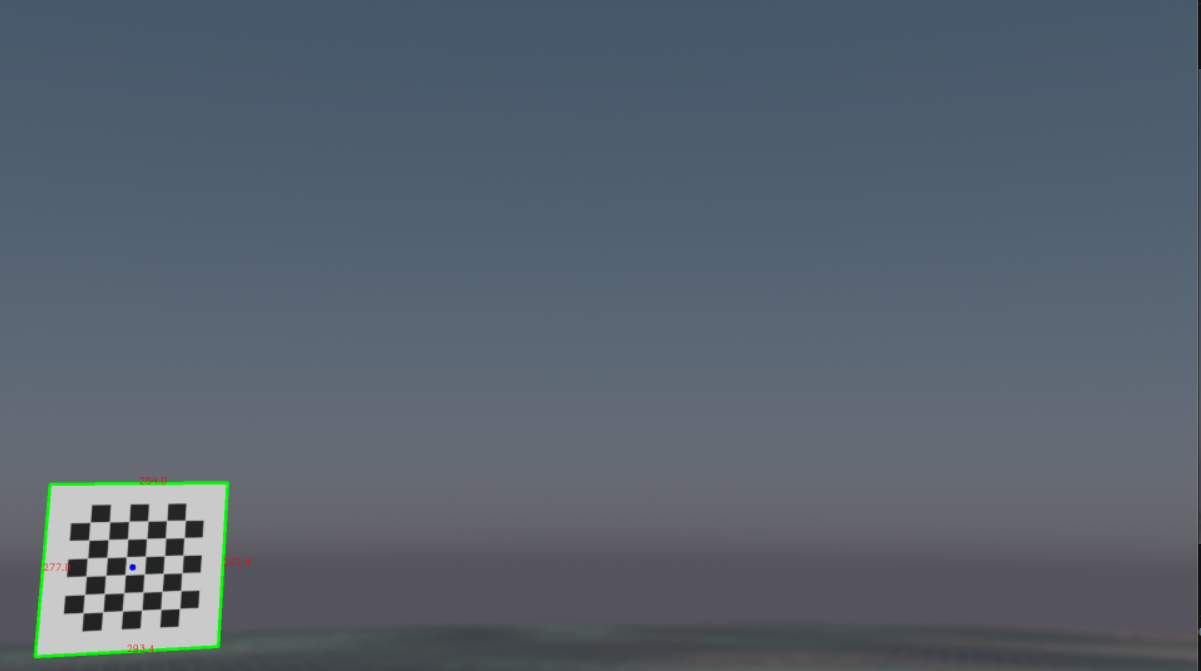
\includegraphics[width=\textwidth]{Images/02stateart/edge_detection_4.png}
        \caption{Image 4}
    \end{subfigure}
    
    \vspace{1cm}
    
    % Third row
    \begin{subfigure}[b]{0.45\textwidth}
        \centering
        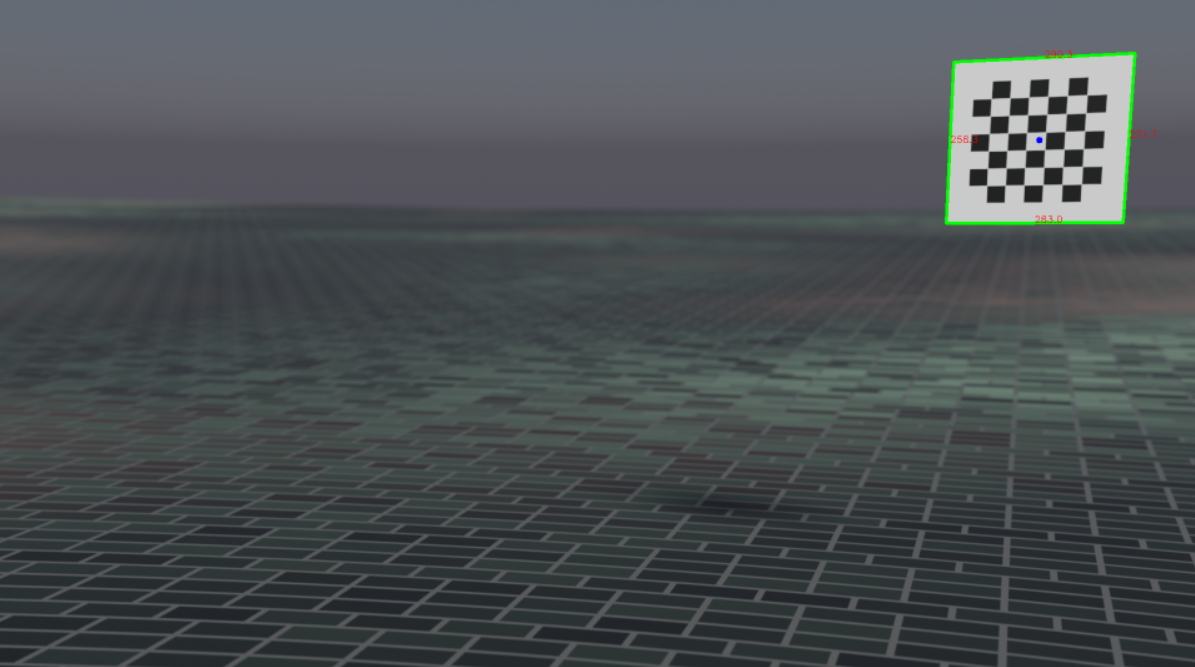
\includegraphics[width=\textwidth]{Images/02stateart/edge_detection_5.png}
        \caption{Image 5}
    \end{subfigure}
    \hfill
    \begin{subfigure}[b]{0.45\textwidth}
        \centering
        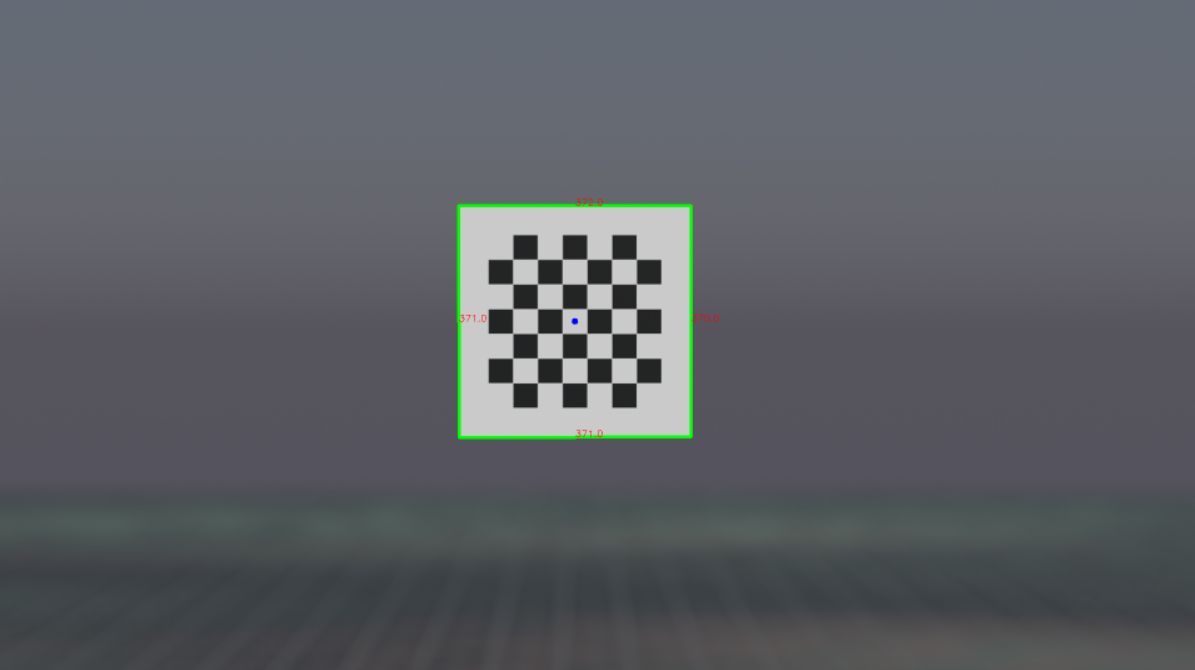
\includegraphics[width=\textwidth]{Images/02stateart/edge_detection_6.png}
        \caption{Image 6}
    \end{subfigure}
    
    \vspace{1cm}
    
    % Fourth row
    \begin{subfigure}[b]{0.45\textwidth}
        \centering
        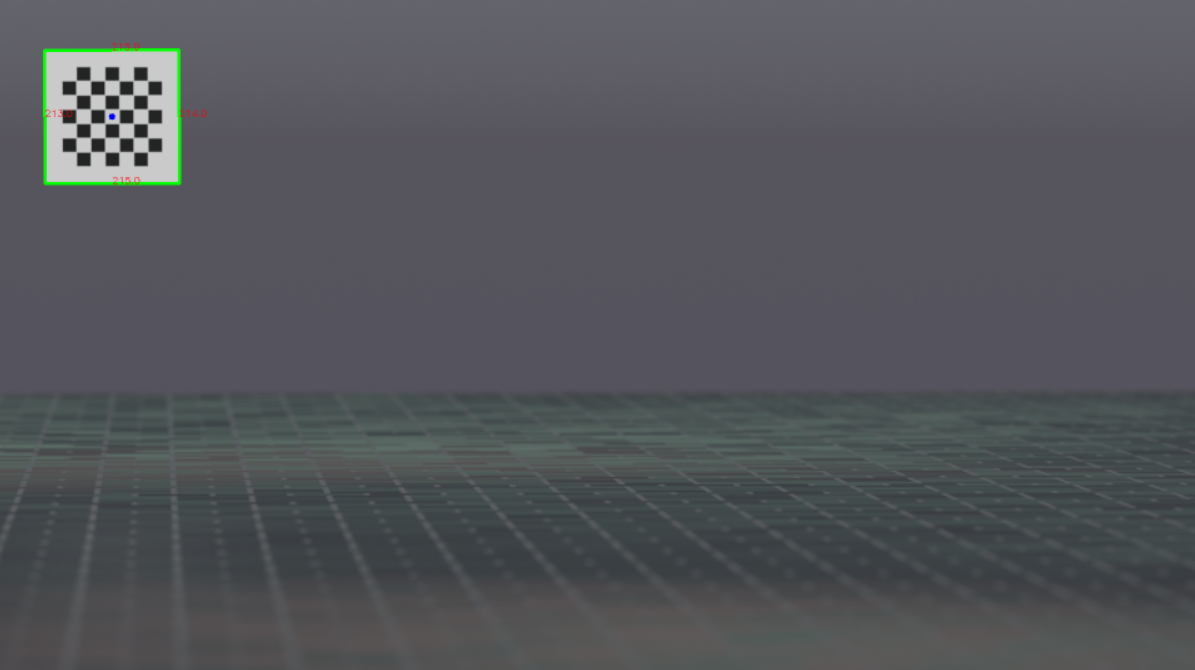
\includegraphics[width=\textwidth]{Images/02stateart/edge_detection_7.png}
        \caption{Image 7}
    \end{subfigure}
    \hfill
    \begin{subfigure}[b]{0.45\textwidth}
        \centering
        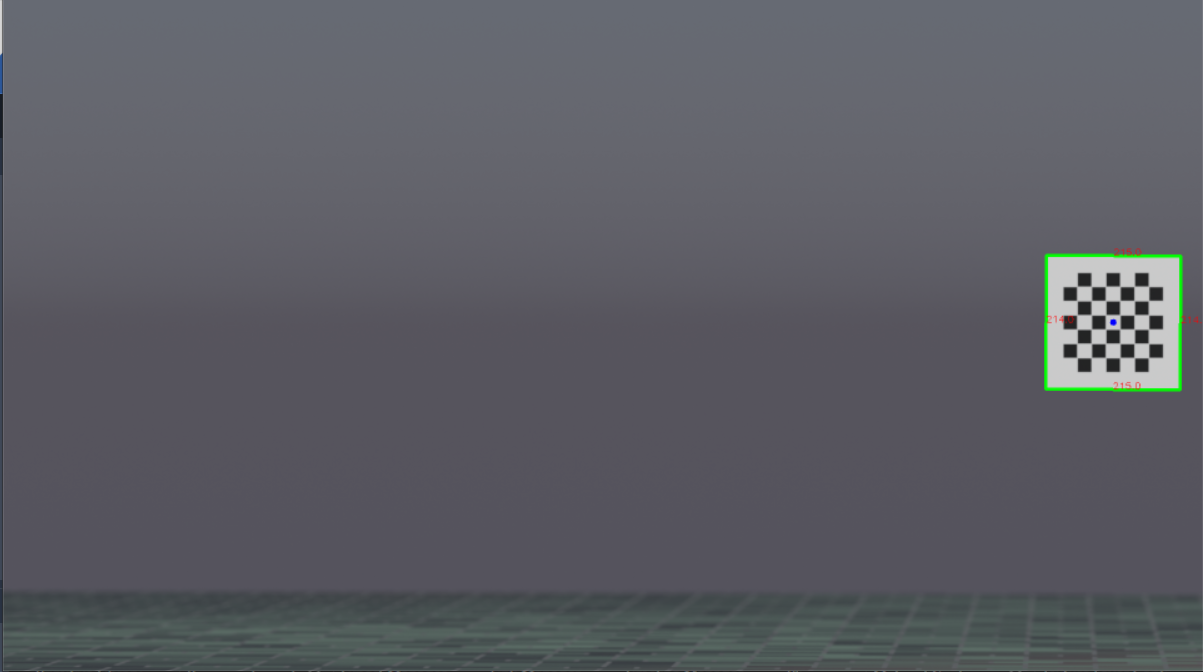
\includegraphics[width=\textwidth]{Images/02stateart/edge_detection_8.png}
        \caption{Image 8}
    \end{subfigure}
    
    \caption{Edge Detection Results Visualization}
    \label{fig:Edge Detection Results Visualization}
\end{figure}

\noindent From these tests, we can confirm that the program works as intended. Even for distorted images.

\noindent This method, however, presents certain limitations. When tested in real-world scenarios, the program occasionally misidentified the real target due to interference from ambient lighting. To mitigate this issue, the target color was changed from white to red, as red is a less common color in real-world environments and contrasts well in studio settings that employ green screens.
\chapter{Camera Lens Calibration} \label{chap:Camera Lens calibration}

\noindent A calibration algorithm that iterativly determines the distortion coefficient was developed. This chapter presents a detail explanation of how it workd. A summary of the results can be seen in Figure \ref{fig:distortion}.

\noindent Virtual images were used for experimentation. These where created using $R^3$ software with known distortion coefficients. 
These images were recreated from the results of a previous calibration done manually at wTVision to ensure realistic values. The 
obtained images where saved in a folder. In this folder, there were images with different zoom and focus levels.
For a specific zoom and focus level, for example Zoom 0 and Focus 0, there were four images, one for each distortion coefficient
that needs to be determined: Center-shift\footnote{Note that even though there is an image for calibrating the center-shift at each level, this is not necessary since for calibrating the center-shift only the zoom matters. In fact, only the images at zoom 0 and at maximum zoom are required. In other words, the same center-shift calibration results can be obtained using images captured at a zoom level of 0 with any focus value within its minimum and maximum range, and another image taken at the maximum zoom level with a focus value.}, \ac{FoV}, K1 and K2.

\noindent The objective is to accuratly determine the distortion coefficients of the (simulated) images. The distortion coefficients are then compared to the real values to evaluate the accuracy of the calibration process.

\noindent Before initiating the calibration process, it is essential to measure the dimensions and position of the real target. The origin of the real-world coordinate system is defined at floor level, directly below the camera's optical point. Using these measurements, a virtual object is inserted into the \( R^3 \) software. Additionally, the pan, roll, and tilt of the camera must all be set to zero.

\section{Center-shift calibration} \label{sec:Center-shift calibration}

\noindent A program capable of accurately detecting the corners of the target in the real world has been developed. In this step the \( R^3 \) software is used to incorporate a virtual object with the same pattern as the real-world target, using the image captured by the camera, to calibrate the center-shift.

\noindent At this stage, a virtual target with accurate dimensions is present in the virtual environment. The first step in the calibration process is determining the center-shift. Experimental validation of the existing calibration procedure has demonstrated that when the camera’s tilt, pan, and roll are set to zero, the center-shift values correspond precisely to the pixel coordinates of the center of the light circle. This conclusion was derived through manual calibration of the center-shift and by using the edge detection program to identify the coordinates of the light circle’s center.

\noindent The center-shift calibration procedure follows a systematic approach. Initially, the camera is set to its minimum zoom level, and the target is positioned at the center of the frame. The image is then focused, and the edge-detection program is utilized to determine the coordinates of the center point. These coordinates are subsequently updated as the new center-shift values. The camera zoom is then adjusted to its maximum level, and the target is refocused to verify the accuracy of the center-shift calibration.

\noindent The center-shift calibration process is illustrated in Figure \ref{fig:main}. The real object is shown in Figure \ref{fig:a}, with the red square representing the target. In Figure \ref{fig:b}, a virtual cone is inserted into the \( R^3 \) software with an uncalibrated center-shift. The center coordinates of the real object are detected in Figure \ref{fig:c}, and the virtual cone is calibrated in Figure \ref{fig:d}. The final result is shown in Figure \ref{fig:f}, with the virtual cone correctly calibrated to the real object. \ref{fig:f} shows the result of changing the pan, tilt and/or roll of an already calibrated center-shift.

\begin{figure}[h]
    \centering
    \begin{subfigure}[b]{0.45\textwidth}
        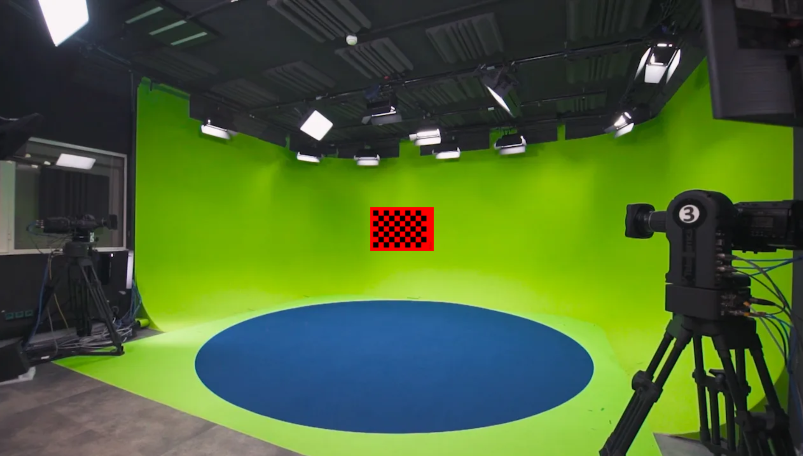
\includegraphics[width=\textwidth]{Images/04calibration/1.png}
        \caption{}
        \label{fig:a}
    \end{subfigure}
    \hfill
    \begin{subfigure}[b]{0.45\textwidth}
        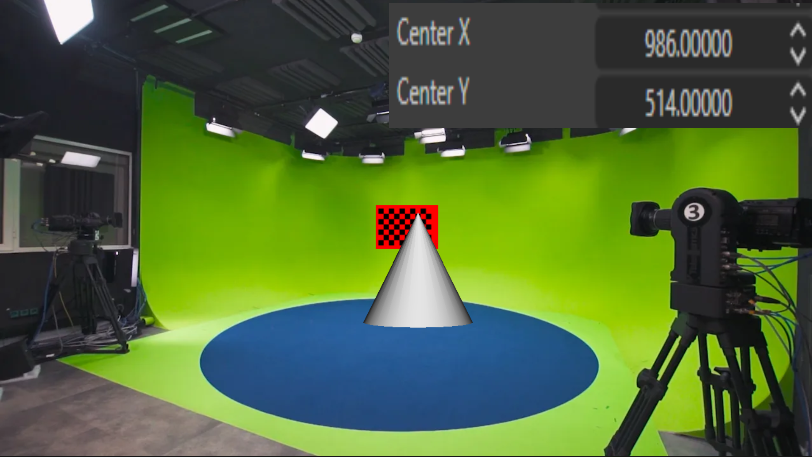
\includegraphics[width=\textwidth]{Images/04calibration/2.png}
        \caption{}
        \label{fig:b}
    \end{subfigure}
    
    \vspace{0.5cm}
    
    \begin{subfigure}[b]{0.45\textwidth}
        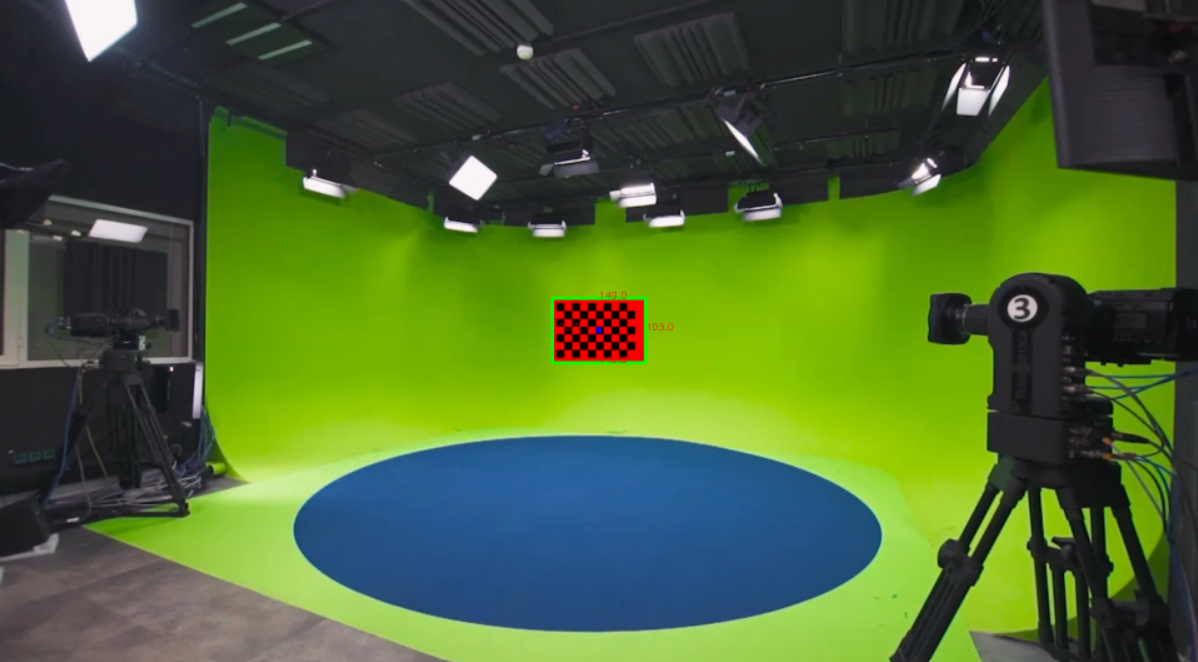
\includegraphics[width=\textwidth]{Images/04calibration/3.png}
        \caption{}
        \label{fig:c}
    \end{subfigure}
    \hfill
    \begin{subfigure}[b]{0.45\textwidth}
        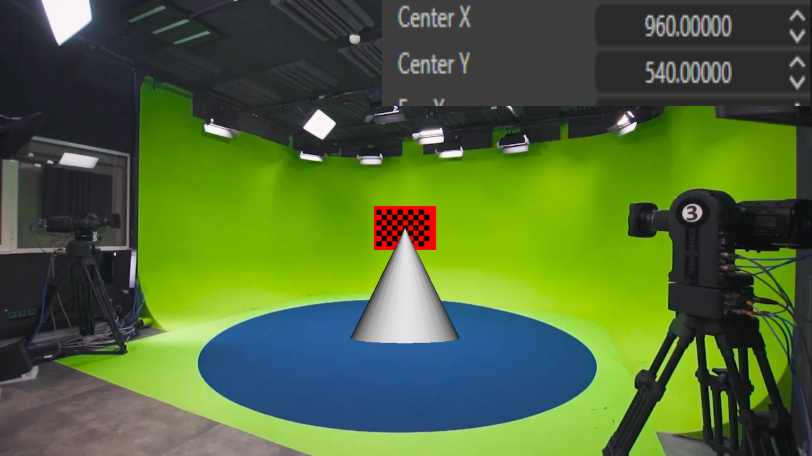
\includegraphics[width=\textwidth]{Images/04calibration/4.png}
        \caption{}
        \label{fig:d}
    \end{subfigure}

    \caption{Example of a center-shift calibration:(a) - Real object (red square) at max zoom, (b) - Insertion of a virtual cone with uncalibrated center-shift, (c) - Detection real object center coordinates, (d) - Calibrated virtual cone.}
    \label{fig:main}
\end{figure}

\begin{figure}[h]
    \centering
    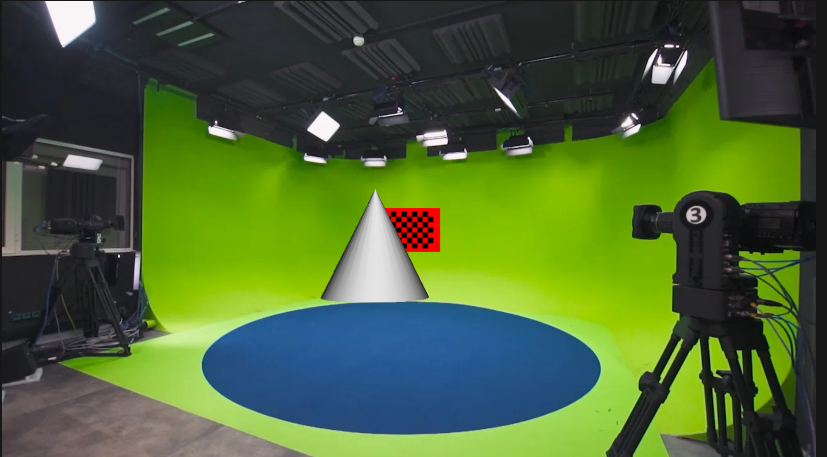
\includegraphics[width=0.45\textwidth]{Images/04calibration/5.png}
    \caption{calibrated center-shift after changing the pan and tilt}
    \label{fig:f}
\end{figure}

\section{ K1, K2 and \ac{FoV} calibration} \label{sec:FoV calibration}

\noindent Following this, the calibration of the \ac{FoV} is performed. The procedure involves applying a pan movement 
to the camera, causing the target to shift laterally within the frame. The edge-detection program is 
then employed to extract the edges of the real target like shown in figure \ref{fig:fov_cal}. Then the background is 
then turned off and the virtual object is inserted, for each iteration the program detectes the corners of the virtual object\footnote{This means that the $R^3$ software has to take and save a snapshot for each iteration. These snapshots are saved and rewritten into the disk which constituites a big limitations in terms of time efficiency.} like shown in 
figure \ref{fig:vir_fov_cal}.  
It has been observed that the virtual object appears narrower than the real target. To achieve proper calibration, the \ac{FoV} value must be adjusted until the virtual and real targets are perfectly aligned. This adjustment is conducted using a program to iteratively increment the \ac{FoV} value until alignment is achieved. To optimize efficiency, the program employs a gradient descent function. A similar approach is utilized for the calibration of distortion parameters \( K_1 \) and \( K_2 \).

\noindent A challenge encountered in this implementation was the misalignment of targets, even when their widths were correctly calibrated. To address this, an improved approach was developed, which calculates the distance between the corner coordinates of the real and virtual objects. Calibration is considered complete when no corner exhibits a deviation beyond a predefined threshold. This method proves more effective than computing the total error across all corners, as summing individual errors does not provide an accurate representation of the alignment quality between the two targets.

\noindent After calibrating the K1 coefficient, determining the \ac{FoV} value would possibly result in a misalignment of the targets. This was resolved by recalibrating the K1 coefficient after adjusting the \ac{FoV} value multiple times until both values are correctly determined. This iterative process ensures that the calibration is accurate and that the targets are correctly aligned. The K2 coefficient is calibrated in a similar manner, with the K1 and K2 values being adjusted iteratively until both coefficients are correctly calibrated.

\begin{figure}[h]
    \centering
    \begin{subfigure}[b]{0.45\textwidth}
        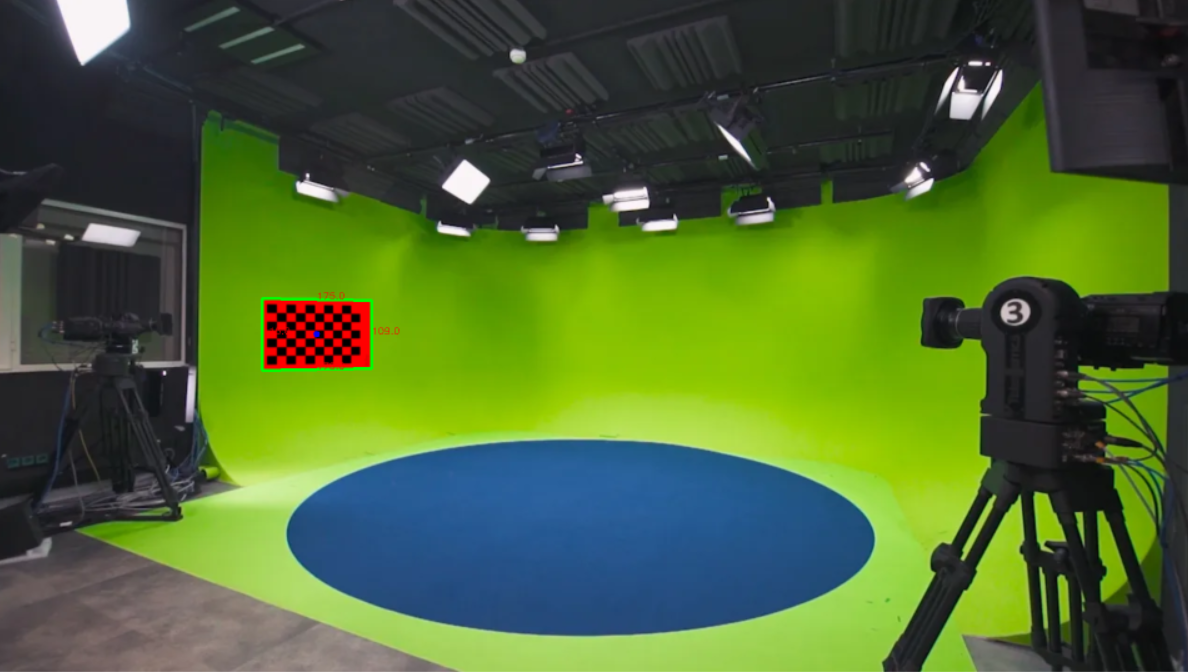
\includegraphics[width=\textwidth]{Images/04calibration/6.png}
        \caption{}
        \label{fig:a1}
    \end{subfigure}
    \hfill
    \begin{subfigure}[b]{0.45\textwidth}
        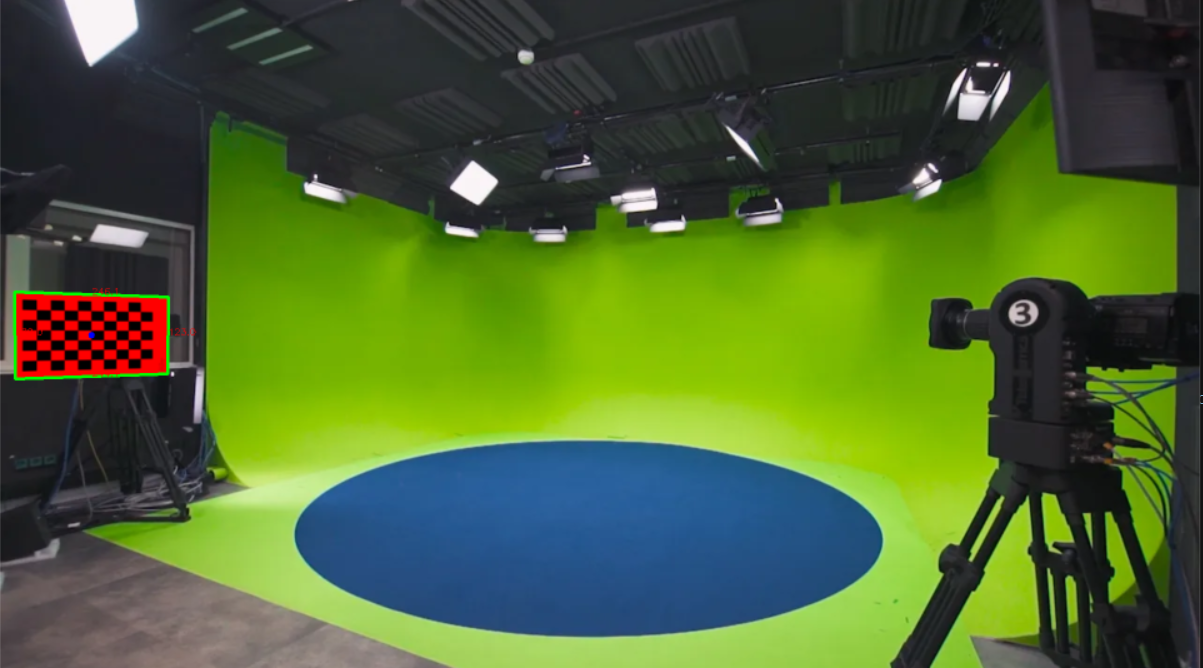
\includegraphics[width=\textwidth]{Images/04calibration/7.png}
        \caption{}
        \label{fig:b1}
    \end{subfigure}
    
    \vspace{0.5cm}
    
    \begin{subfigure}[b]{0.45\textwidth}
        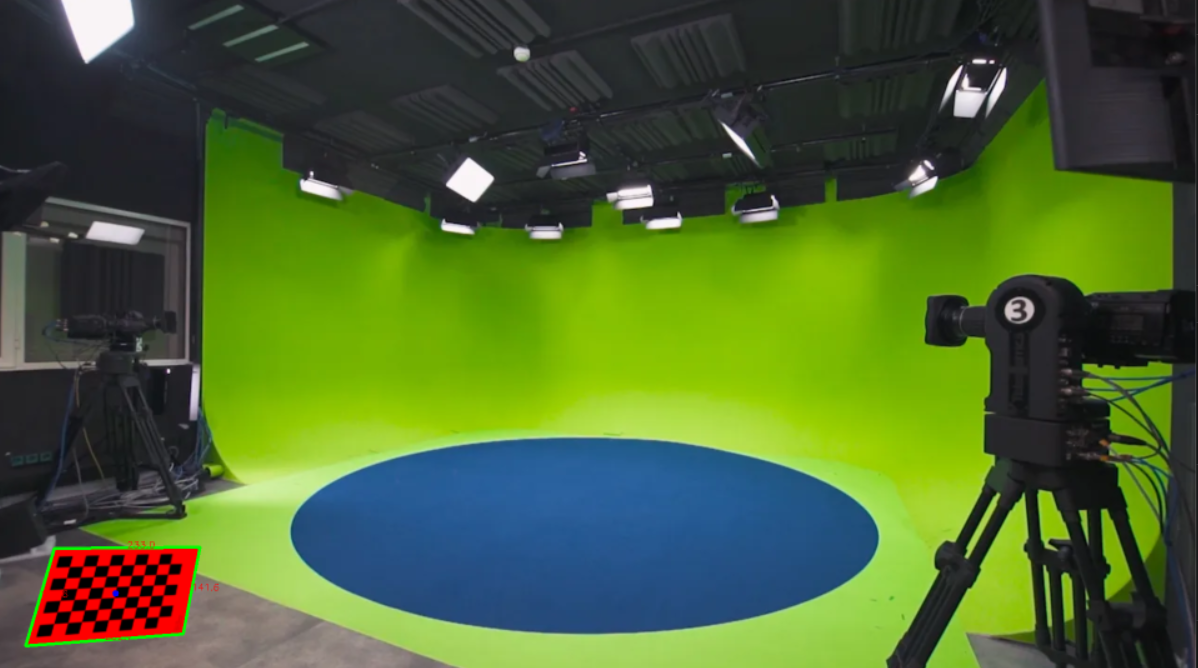
\includegraphics[width=\textwidth]{Images/04calibration/8.png}
        \caption{}
        \label{fig:c1}
    \end{subfigure}

    \caption{Example of K1, K2 and \ac{FoV} calibration using edge detection to determine the real object corners coordinates: (a) - \ac{FoV} calibration, (b) - K1 calibration, (c) - K2 calibration.}
    \label{fig:fov_cal}
\end{figure}

\begin{figure}[h]
    \centering
    \begin{subfigure}[b]{0.45\textwidth}
        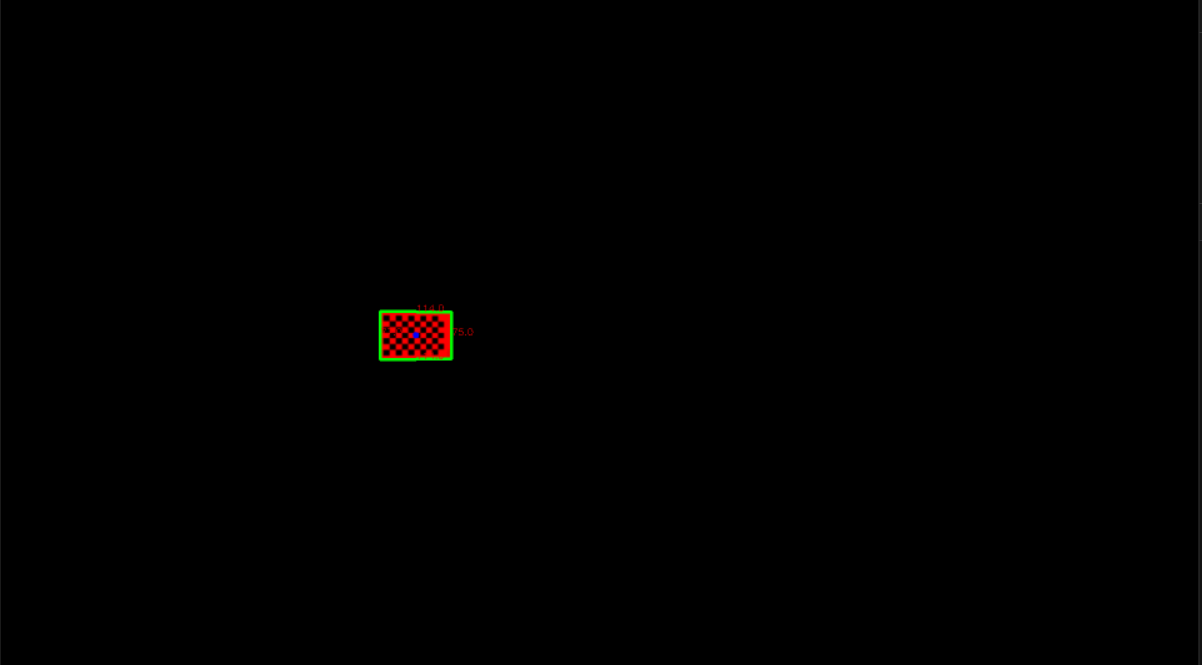
\includegraphics[width=\textwidth]{Images/04calibration/9.png}
        \caption{}
        \label{fig:a2}
    \end{subfigure}
    \hfill
    \begin{subfigure}[b]{0.45\textwidth}
        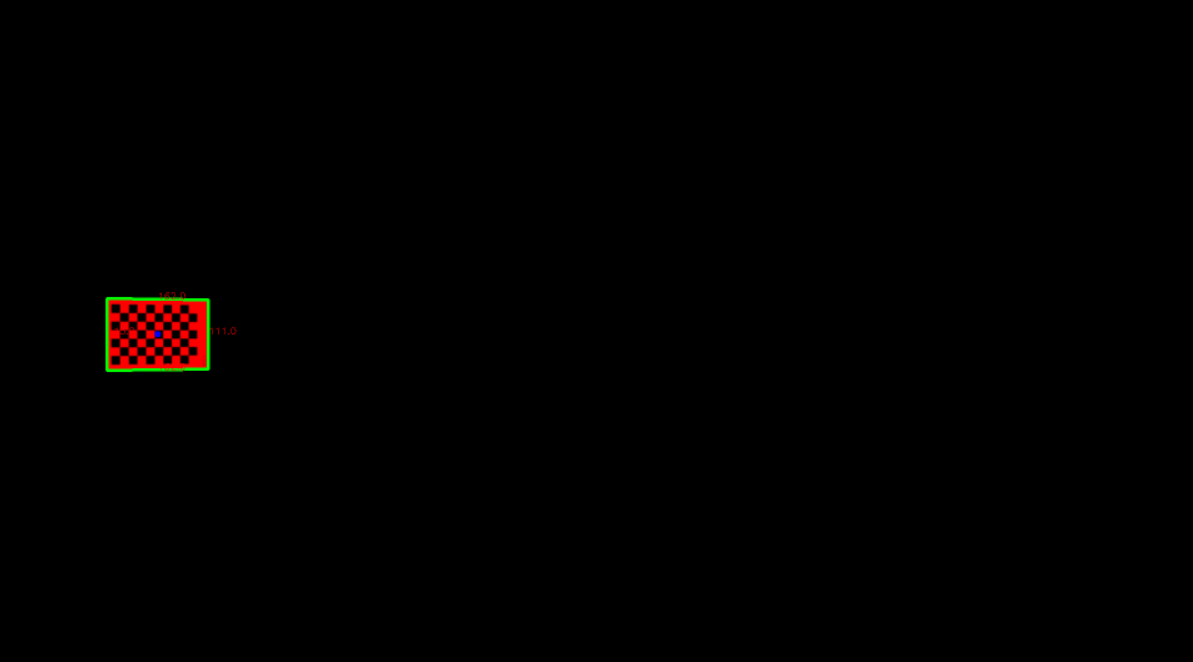
\includegraphics[width=\textwidth]{Images/04calibration/10.png}
        \caption{}
        \label{fig:b2}
    \end{subfigure}
    
    \vspace{0.5cm}
    
    \begin{subfigure}[b]{0.45\textwidth}
        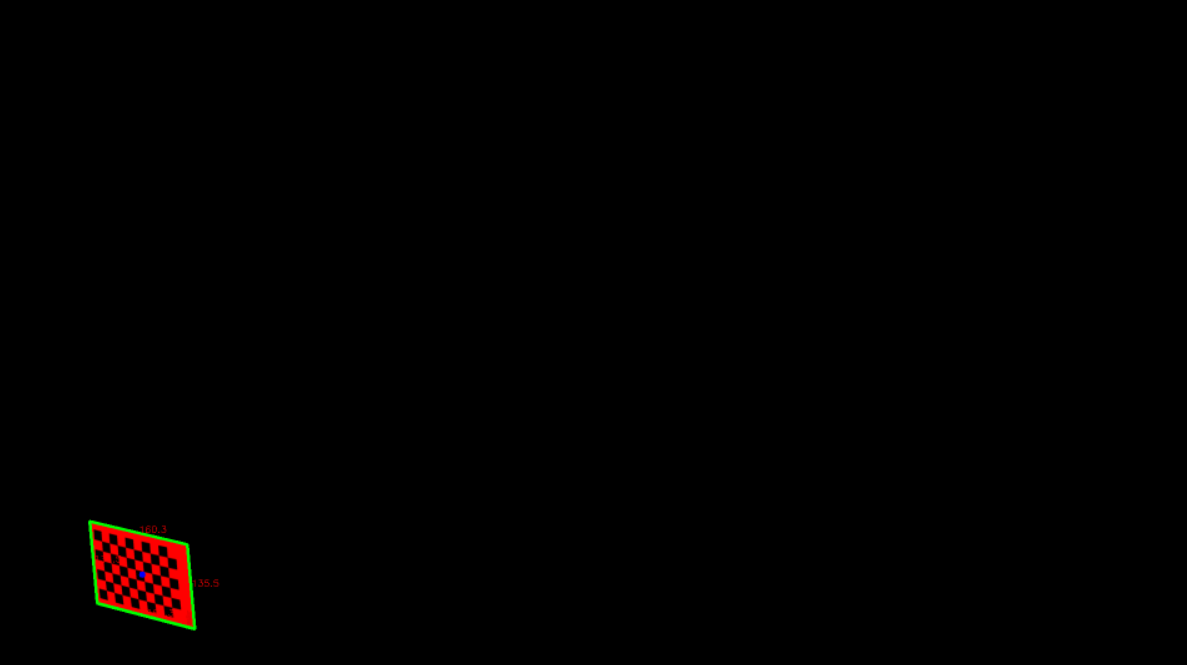
\includegraphics[width=\textwidth]{Images/04calibration/11.png}
        \caption{}
        \label{fig:c2}
    \end{subfigure}

    \caption{Example of K1, K2 and \ac{FoV} calibration using edge detection to determine the virtual object corners coordinates: (a) - \ac{FoV} calibration, (b) - K1 calibration, (c) - K2 calibration.}
    \label{fig:vir_fov_cal}
\end{figure}




\section{Calibration Scenarios} \label{sec:Calibration Scenarios}

\noindent The calibration process using the algorithm follows the same principles as manual calibration. First, it calibrates the \ac{FoV} to the best possible value. Then, it calibrates the K1 coefficient, iteratively refining both until they reach their optimal values. Afterward, the K2 calibration is performed using a similar iterative approach, adjusting both K1 and K2 until they are optimally calibrated.

\noindent After completing these steps, the algorithm’s results could be categorized into three scenarios:

\begin{itemize}
    \item \textbf{Scenario 1:} The \ac{FoV} and K1 are correctly calibrated, and K2 is extremely close to 0. In this case, the effect of K2 is negligible. To optimize time efficiency, the algorithm is modified to stop if the K1 and \ac{FoV} coefficients are already correctly calibrated. This is the most common scenario in real-world applications at most levels of calibration.
    
    \item \textbf{Scenario 2:} The K1 and \ac{FoV} are not correctly determined, indicating that the K2 coefficient is not negligible. In this case, the algorithm proceeds to calibrate the K2 coefficient.
    
    \item \textbf{Scenario 3:} After calibrating the K2 coefficient, if the K1 and K2 coefficients are still not correctly calibrated, the algorithm may have become stuck, recalibrating to the same values repeatedly. To resolve this issue, the algorithm is modified to detect this scenario and forcibly adjust the K1 value before recalibrating K2 until both coefficients are correctly calibrated.
\end{itemize}

\noindent The program effectively determines the distortion coefficients with satisfactory accuracy. However, the calibration process is time-consuming, taking approximately 65 minutes to complete six levels, which is impractical for efficient operation. In the next chapter, we will explore strategies to optimize and reduce the calibration time.

\section{Results} \label{sec:Results}

\begin{figure}[ht]
    \centering
    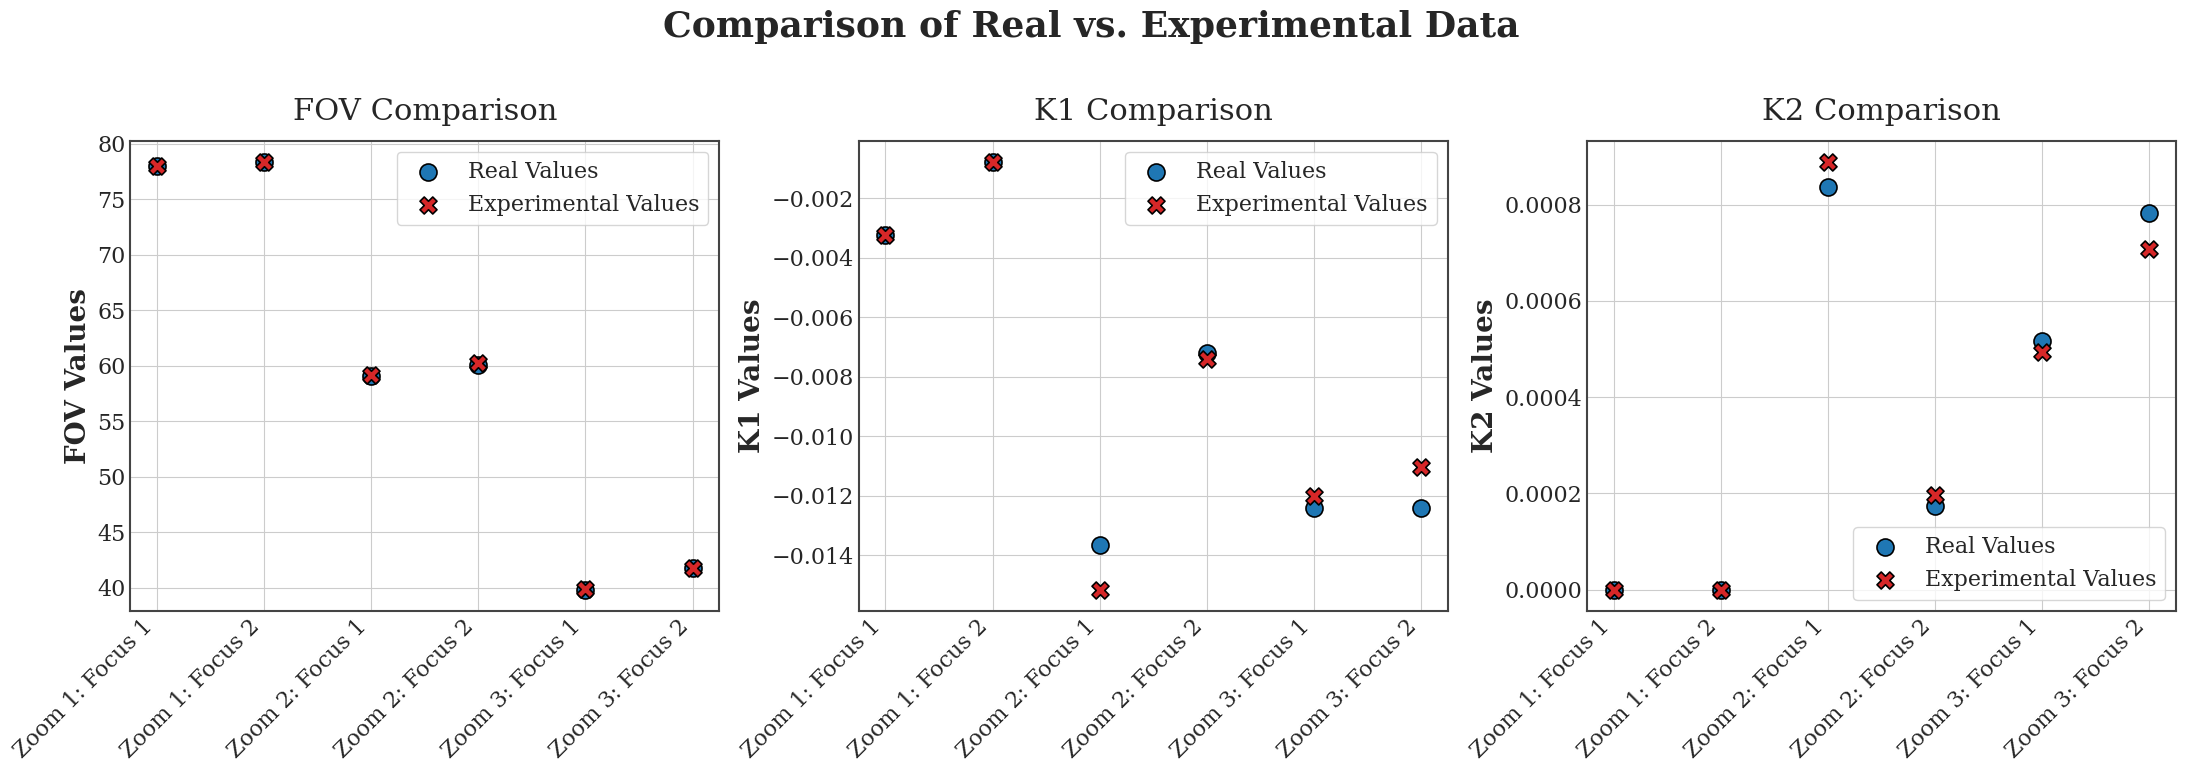
\includegraphics[width=1.1\textwidth]{Images/04calibration/novos_resul.png}
    \caption{Distortion calibration results}
    \label{fig:distortion}
\end{figure}





\chapter{Optimizing Calibration Efficiency} \label{chap:Time}

\noindent This chapter explores strategies to reduce the calibration time of the algorithm. The initial approach involved transcribing the algorithm from Python to C++ to leverage the latter’s greater computational efficiency. However, despite the significant development effort required, this optimization yielded only a marginal improvement, reducing calibration time by approximately 1\%.

\noindent Given the limited success of this approach, an alternative solution was pursued. It was identified that the primary bottleneck in the program was the process of saving snapshots to the computer’s disk during each iteration, which significantly slowed down execution. To address this, a virtual graphics card provided by wTVision was utilized, enabling direct communication with Python and allowing snapshots to be transferred in real-time instead of being stored on disk. This modification substantially improved the calibration efficiency.

\section{MockBoard} \label{sec:MockBoard}   

\noindent The MockBoard is a virtual graphics card provided by wTVision that allows for the real-time transfer of images to the computer. This eliminates the need to save snapshots to disk, which significantly 
reduces the time required for calibration. The MockBoard is a software solution that emulates a video capture card, enabling the computer to receive video input directly from the $R^3$ software. This allows the computer to process the 
iamges in real-time, without the need to save snapshots to disk. The MockBoard is a proprietary software solution developed by wTVision, and is not available to the general public. 

\noindent To use Mockboard in the calibration algorithm, the following steps are required:

\begin{enumerate}
    \item Open the $R^3$ software in administrator mode.
    \item Select MockBoard as the output in the $R^3$ software, like in figure \ref{fig:MockBoard}.
\end{enumerate}

\begin{figure}[h]
    \centering
    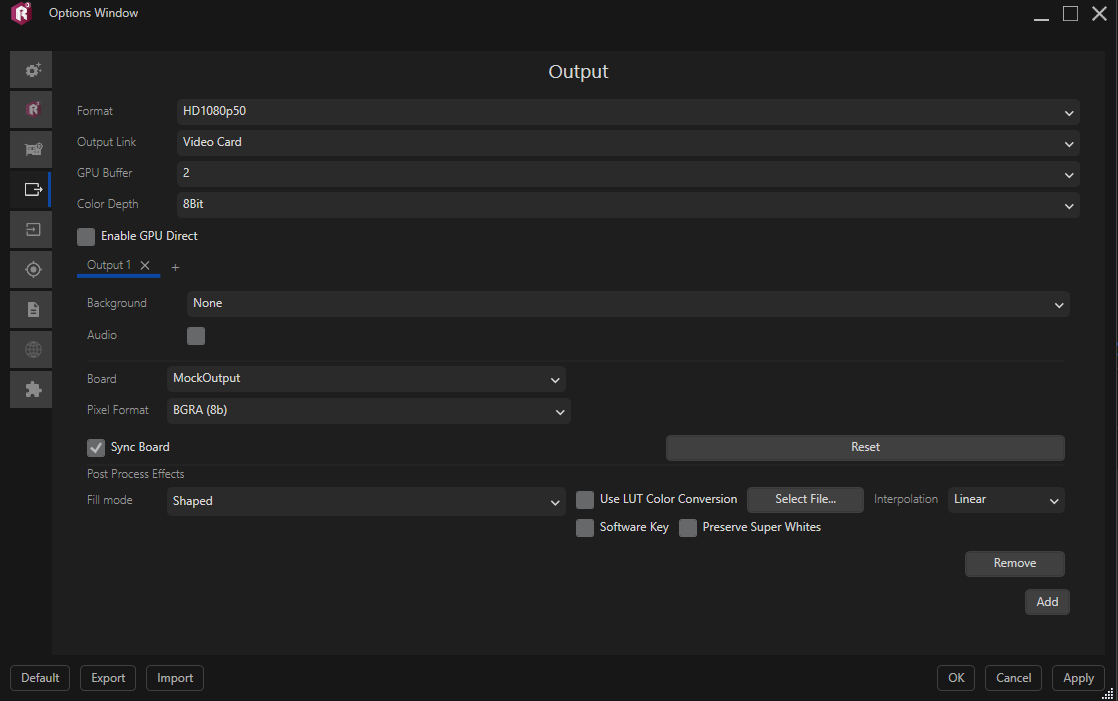
\includegraphics[width=\textwidth]{Images/05optimize/Mockboard.png}
    \caption{Selecting MockBoard as the output in the $R^3$ software.}
    \label{fig:MockBoard}
\end{figure}

\subsection{Communication with MockBoard} \label{subsec:MockBoardComm}

\noindent The MockBoard functions as a local webapi with the following url:

"http://localhost:1987/apiv1/MockCard/MockOutput/GetImage"

\noindent Figure \ref{fig:webapi} illustrates its corresponding web page. 

\begin{figure}[h]
    \centering
    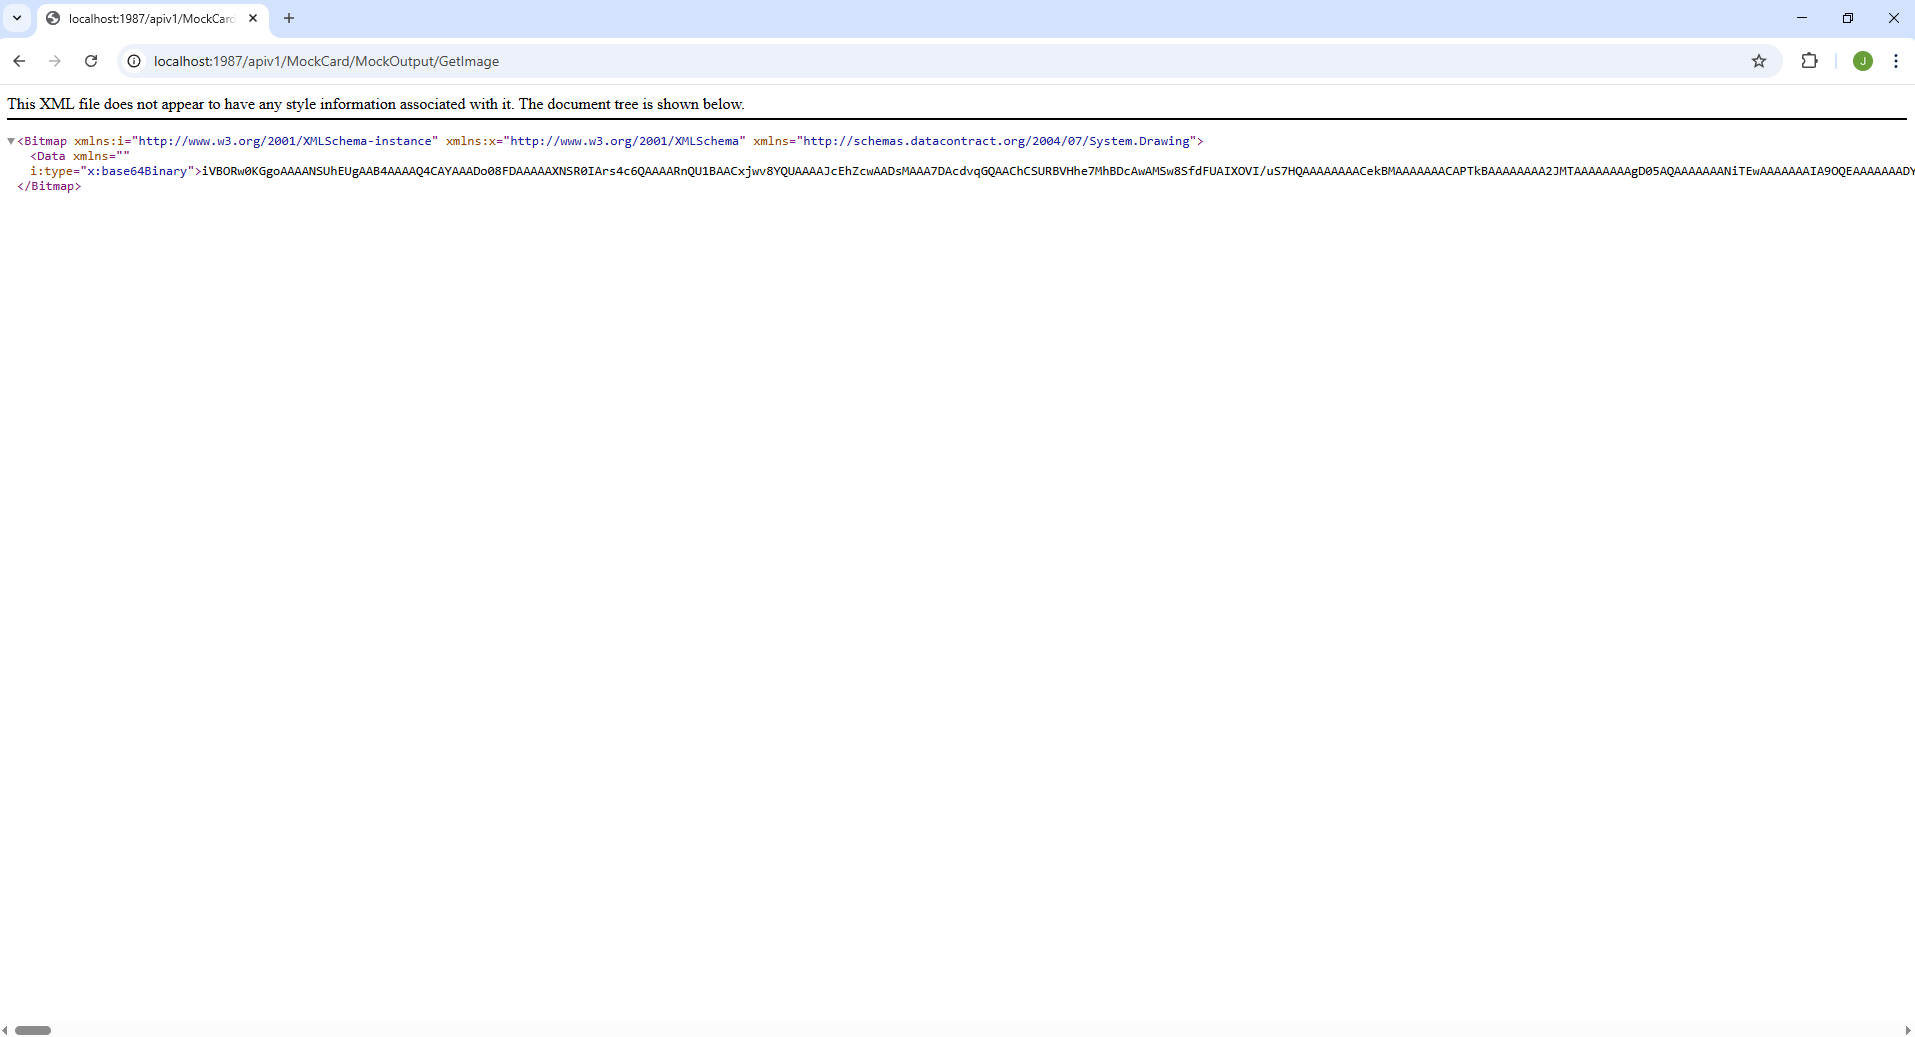
\includegraphics[width=\textwidth]{Images/05optimize/webapi.png}
    \caption{MockBoard web page.}
    \label{fig:webapi}
\end{figure}

\noindent As demonstrated in figure \ref{fig:webapi}, this url returns a string of an image in base64 format.
To communicate with it using Python, http requests are used in order to return this string. The following steps outline how to estaplish communcation between the 
Python script and the MockBoard:


\begin{enumerate}
    \item First, the correct headers need to be added. This can be achieved by using the following code:
    
    \begin{verbatim}
    response = requests.get(url, headers=headers)
    \end{verbatim}
    
    These headers are displayed in Table~\ref{tab:headers} in the annex chapter~\ref{chap:annex}.

    \item Using HTTP requests it is possible to obtain the image in base64 format.
    \item The base64 image is then converted into a png image using the base64 and BytesIO Python libraries.
\end{enumerate}


Using the MockBoard, it takes exacly 0.015 seconds to obtain an image, which is a significant improvement over the previous method of saving snapshots to disk, which took around 0.3 seconds. This 
improvement should reduce the algorithm's calibration time by at least 90\%.

\section{Results} \label{sec:Results}

\noindent The calibration algorithm was tested using the MockBoard to evaluate the impact on calibration time. The results are presented in figure \ref{fig:results}.

\begin{figure}[ht]
    \centering
    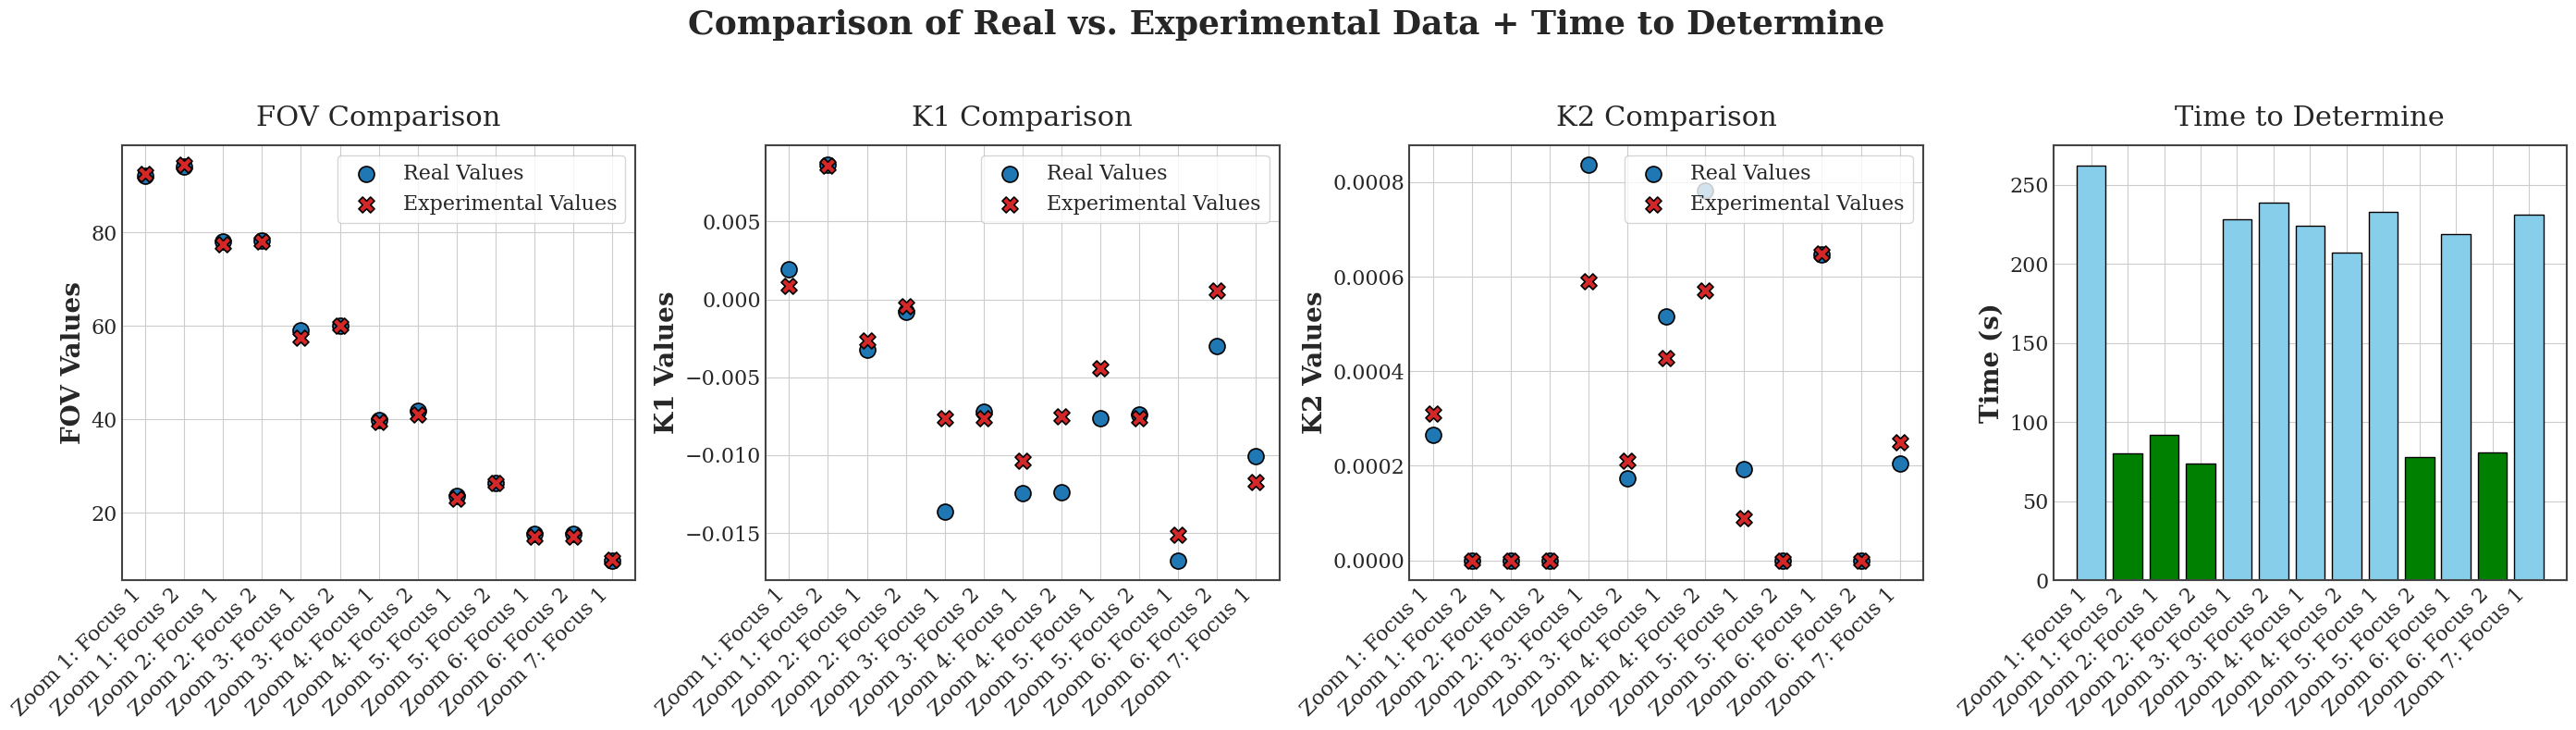
\includegraphics[width=\textwidth]{Images/05optimize/r_graph.png}
    \caption{Distortion calibration results using the MockBoard.}
    \label{fig:results}
\end{figure}

\noindent As shown in figure \ref{fig:results}, the calibration time was significantly reduced, only taking 35.1 minutes to calibrate 13 levels of zoom/focus, 
using the old method would've taken above 120 minutes. This significant improvement in efficiency demonstrates the potential 
of the MockBoard to optimize the calibration algorithm.

\noindent As expected, when K2 is 0 it takes less time to calibrate. The green bars in figure \ref{fig:results} represent the time taken to calibrate when K2 is 0, while the blue bars represent the 
time taken to calibrate when K2 is not 0.
\chapter{Image Deblurring NN} \label{chap:Time}

In real world applications, the images are often blurred due to, mainly, out-of-focus camera.
For the calibration algorithm, a minimum image quality is required to estimate the camera parameters.
To improve the image quality, we can use a deblurring algorithm. In this chapter, we will discuss the deblurring algorithm and 
its implementation using a neural network.

\section{Dataset}

The dataset used for training the neural network is a set of blurred images and their corresponding sharp images. 
These images were obtained using blender, since its able to recreate accurate images of an out-of-focus camera.
Using a python script generated xxxx set of blurred and the corresponding sharp images. Each image consists of a red chessboard square 
with random size, position and aspect ratio with a random studio in the background.

\section{Deblurring using EDSR}

For the deblurring task, we used the Enhanced Deep Super-Resolution (EDSR) network, originally designed for single-image 
super-resolution. Although EDSR was developed to upscale low-resolution images to high-resolution outputs, it has been shown to 
be effective for image restoration tasks such as deblurring.

EDSR is a deep convolutional neural network that removes unnecessary modules, such as batch normalization layers, from its 
predecessor models (e.g., SRResNet) to improve performance. It consists of multiple residual blocks without downsampling, enabling the network 
to maintain spatial information and focus on learning fine details.

In our case, the input to the EDSR network is a blurred image, and the output is its deblurred (sharpened) version. The network is trained to 
minimize the pixel-wise loss between the predicted deblurred image and the ground truth sharp image.

By using EDSR, we benefit from a powerful architecture capable of restoring image details that were lost due to blur, thus enabling better 
performance in downstream tasks such as camera calibration.

\subsection{Loss Function}

Since the images used are very blured, simply using EDSR was not be enough. To tackle this problem,
the algorithm is trained to focus on debluring the chessboard square, which is the only area of interest in the image, giving
little value to the rest of the image. 

This is done by recording the corners coordinates of the chessboard square in the training dataset. By applying a crop on the image blured and 
sharp images. By using the MSELoss function, the algorithm will learn to deblur the chessboard square. In order to not ignore completely
the rest of the image, the algorithm also learns to deblur the rest of the image, but with a lower weight. This is done
by multiplying the MSELoss score of the chessboard square 0.9, and the rest of the image by 0.1 and then adding both.

*The loss functions is not converging this way, alternative needed*




\chapter{Conclusions and Future Work}\label{chap:conclusions}



\chapter{Annexs}\label{chap:annex}

\section{HTTP Headers}

\begin{longtable}{|l|p{12cm}|} 
    \caption{HTTP Headers Used in the Request} \label{tab:headers} \\
    \hline
    \textbf{Header} & \textbf{Value} \\
    \hline
    \endfirsthead

    \hline
    \textbf{Header} & \textbf{Value} \\
    \hline
    \endhead

    \hline
    \endfoot

    \hline
    \endlastfoot

    Accept & text/html, application/xhtml+xml, application/xml;q=0.9, image/avif, image/webp, image/apng, */*;q=0.8, application/signed-exchange;v=b3;q=0.7 \\
    \hline
    Accept-Encoding & gzip, deflate, br, zstd \\
    \hline
    Accept-Language & pt-PT, pt;q=0.9, en-US;q=0.8, en;q=0.7 \\
    \hline
    Cache-Control & max-age=0 \\
    \hline
    Connection & keep-alive \\
    \hline
    Host & localhost:1987 \\
    \hline
    Sec-Fetch-Dest & document \\
    \hline
    Sec-Fetch-Mode & navigate \\
    \hline
    Sec-Fetch-Site & none \\
    \hline
    Sec-Fetch-User & ?1 \\
    \hline
    Upgrade-Insecure-Requests & 1 \\
    \hline
    User-Agent & Mozilla/5.0 (Windows NT 10.0; Win64; x64) AppleWebKit/537.36 (KHTML, like Gecko) Chrome/133.0.0.0 Safari/537.36 \\
    \hline
    sec-ch-ua & "Not(A:Brand";v="99", "Google Chrome";v="133", "Chromium";v="133") \\
    \hline
    sec-ch-ua-mobile & ?0 \\
    \hline
    sec-ch-ua-platform & "Windows" \\
    \hline
\end{longtable}


\section{Calibration Results}

\begin{figure}[h]
    \centering
    \begin{subfigure}[b]{0.45\textwidth}
        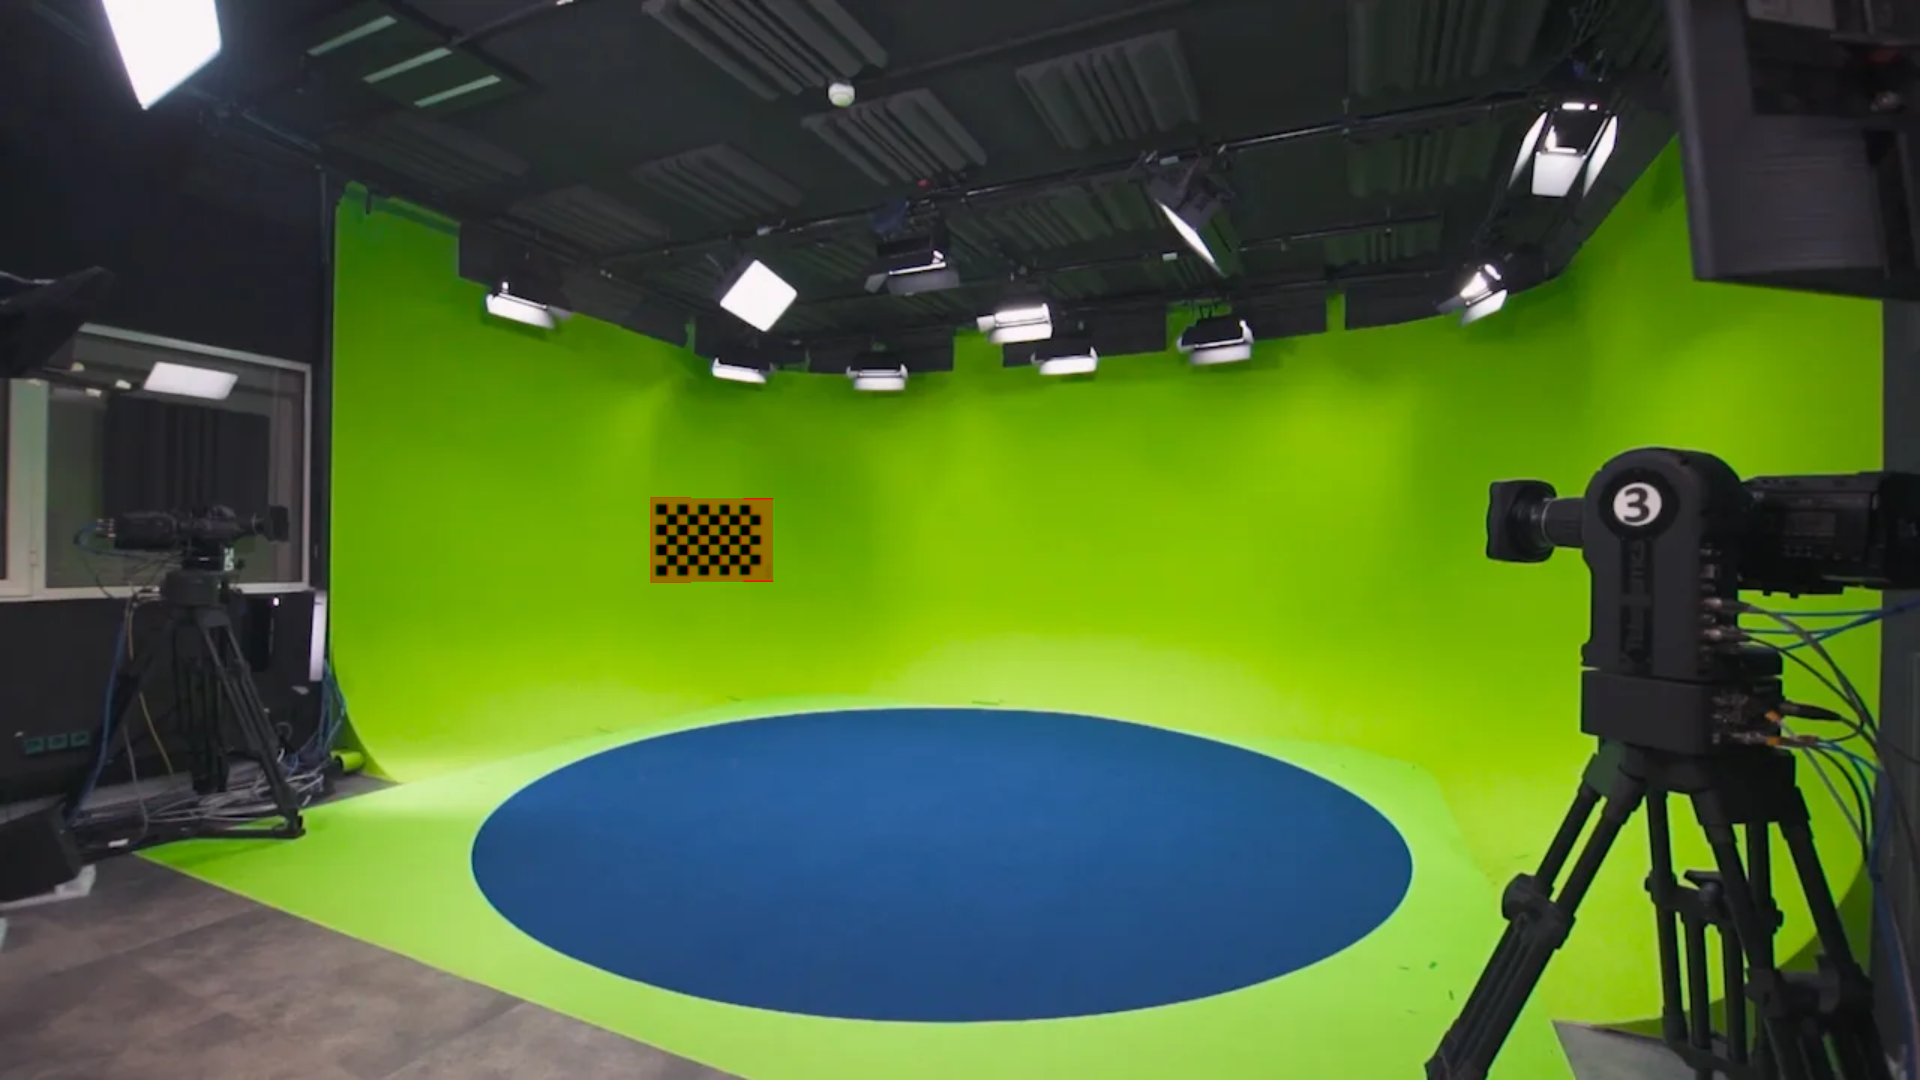
\includegraphics[width=\textwidth]{Images/08annex/results/1.2.png}
        \caption{}
        \label{fig:a2}
    \end{subfigure}
    \hfill
    \begin{subfigure}[b]{0.45\textwidth}
        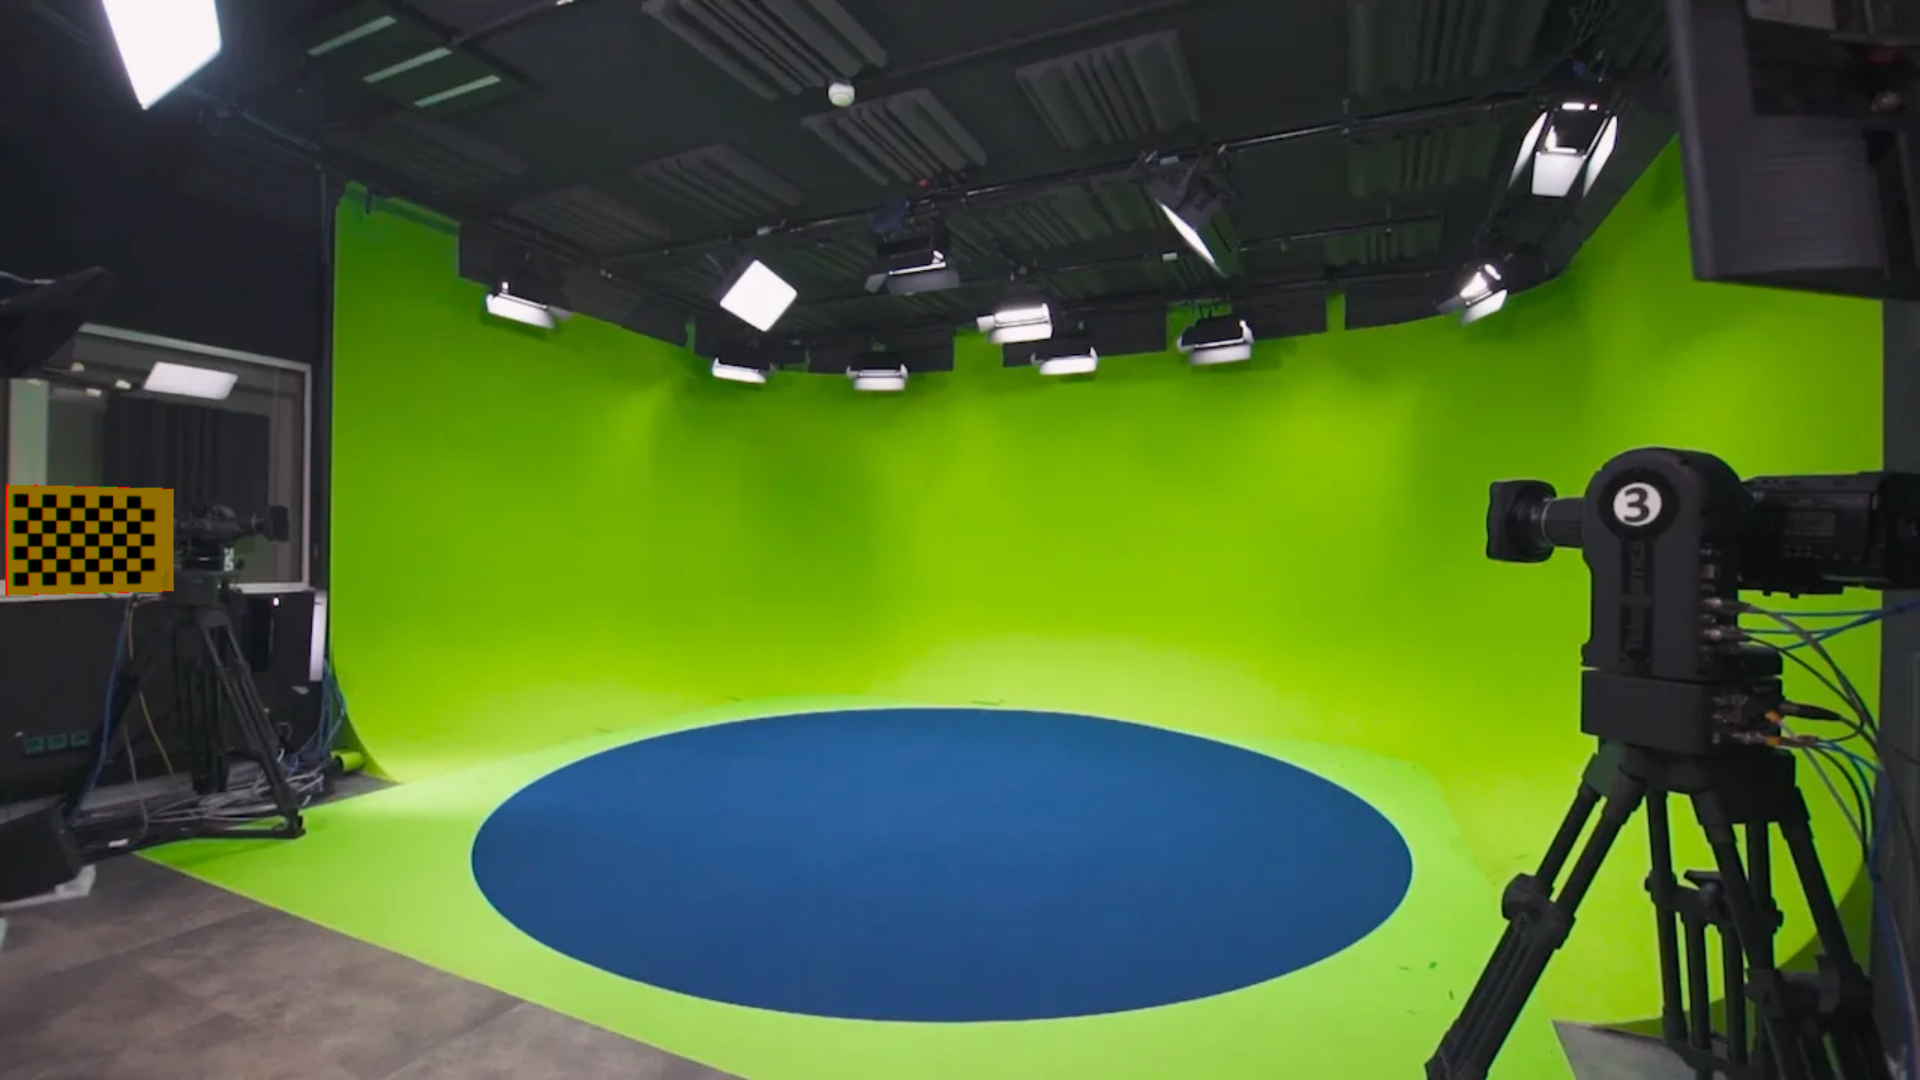
\includegraphics[width=\textwidth]{Images/08annex/results/1.3.png}
        \caption{}
        \label{fig:b2}
    \end{subfigure}
    
    \vspace{0.5cm}
    
    \begin{subfigure}[b]{0.45\textwidth}
        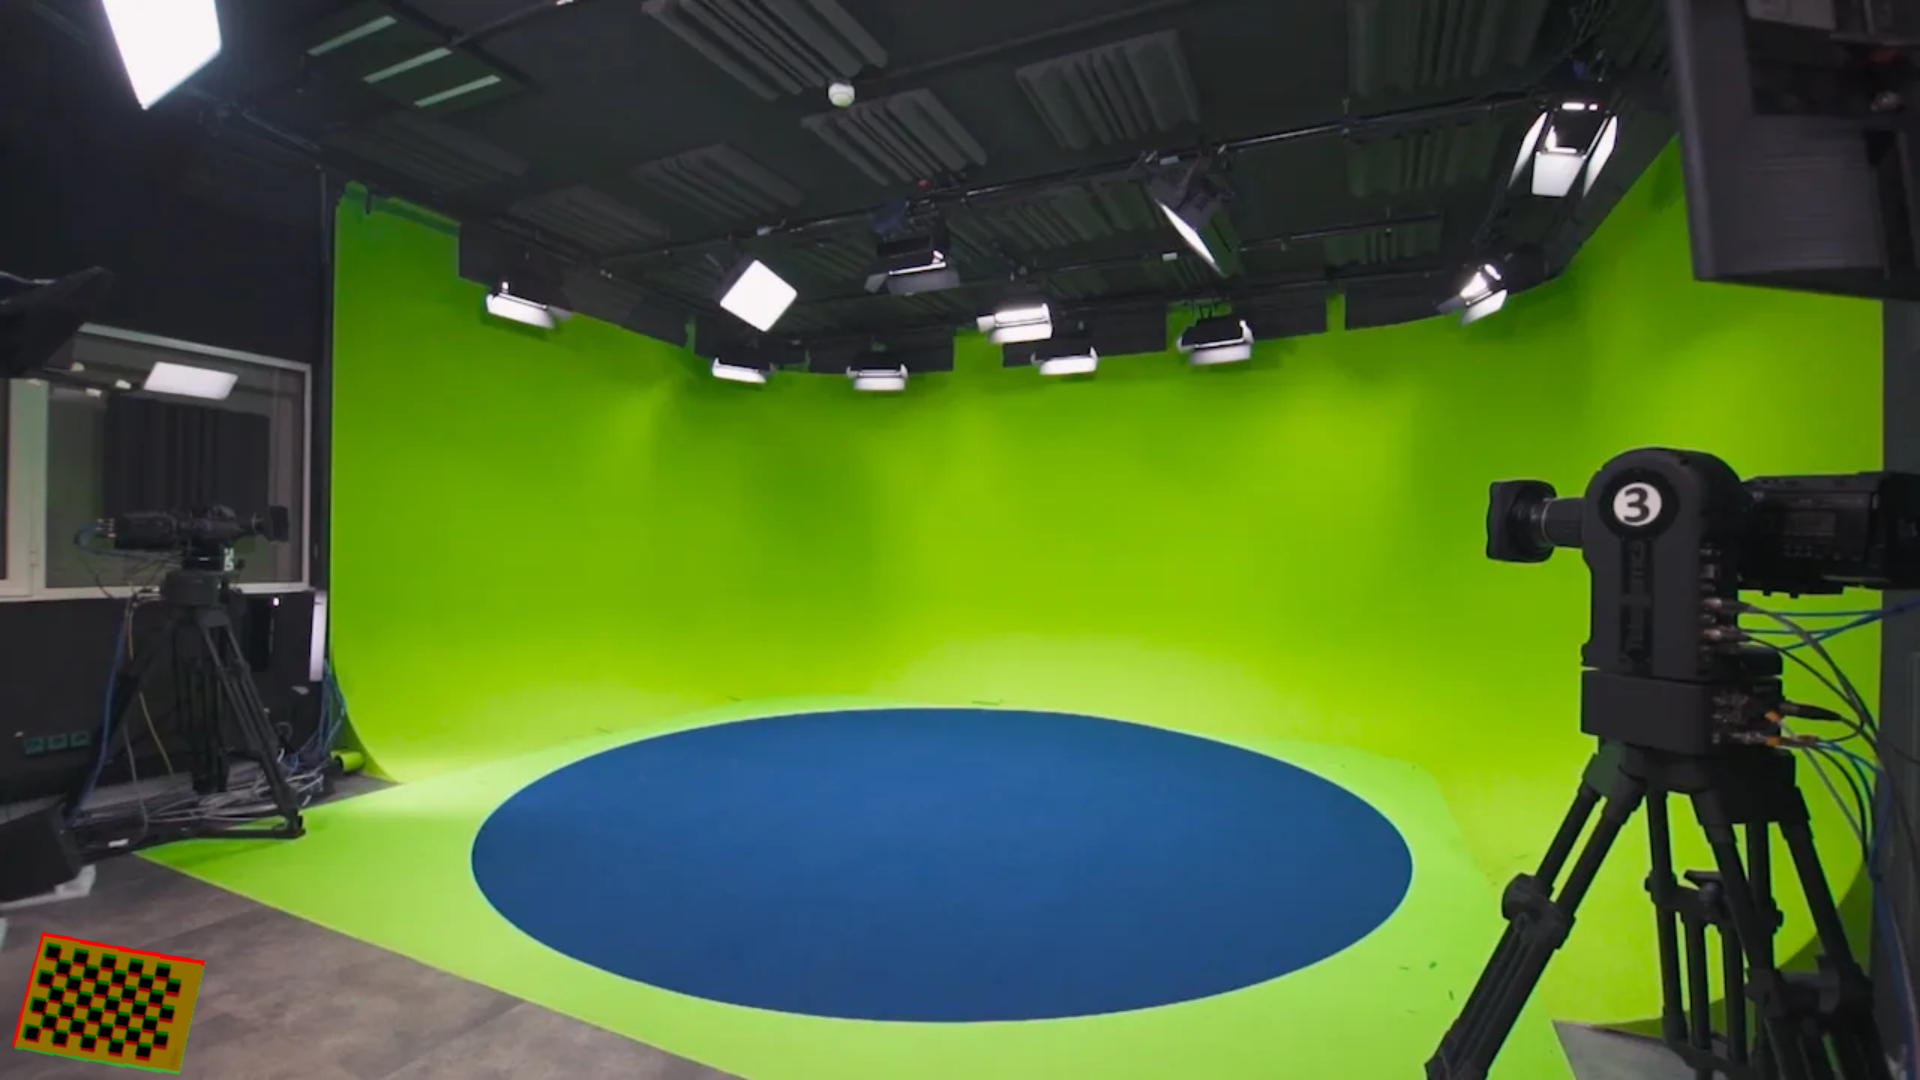
\includegraphics[width=\textwidth]{Images/08annex/results/1.4.png}
        \caption{}
        \label{fig:c2}
    \end{subfigure}

    \caption{Zoom 1 Focus 1 - (a) FoV, (b) K1, (c) K2.}
    \label{fig:vir_fov_cal}
\end{figure}

\begin{figure}[h]
    \centering
    \begin{subfigure}[b]{0.45\textwidth}
        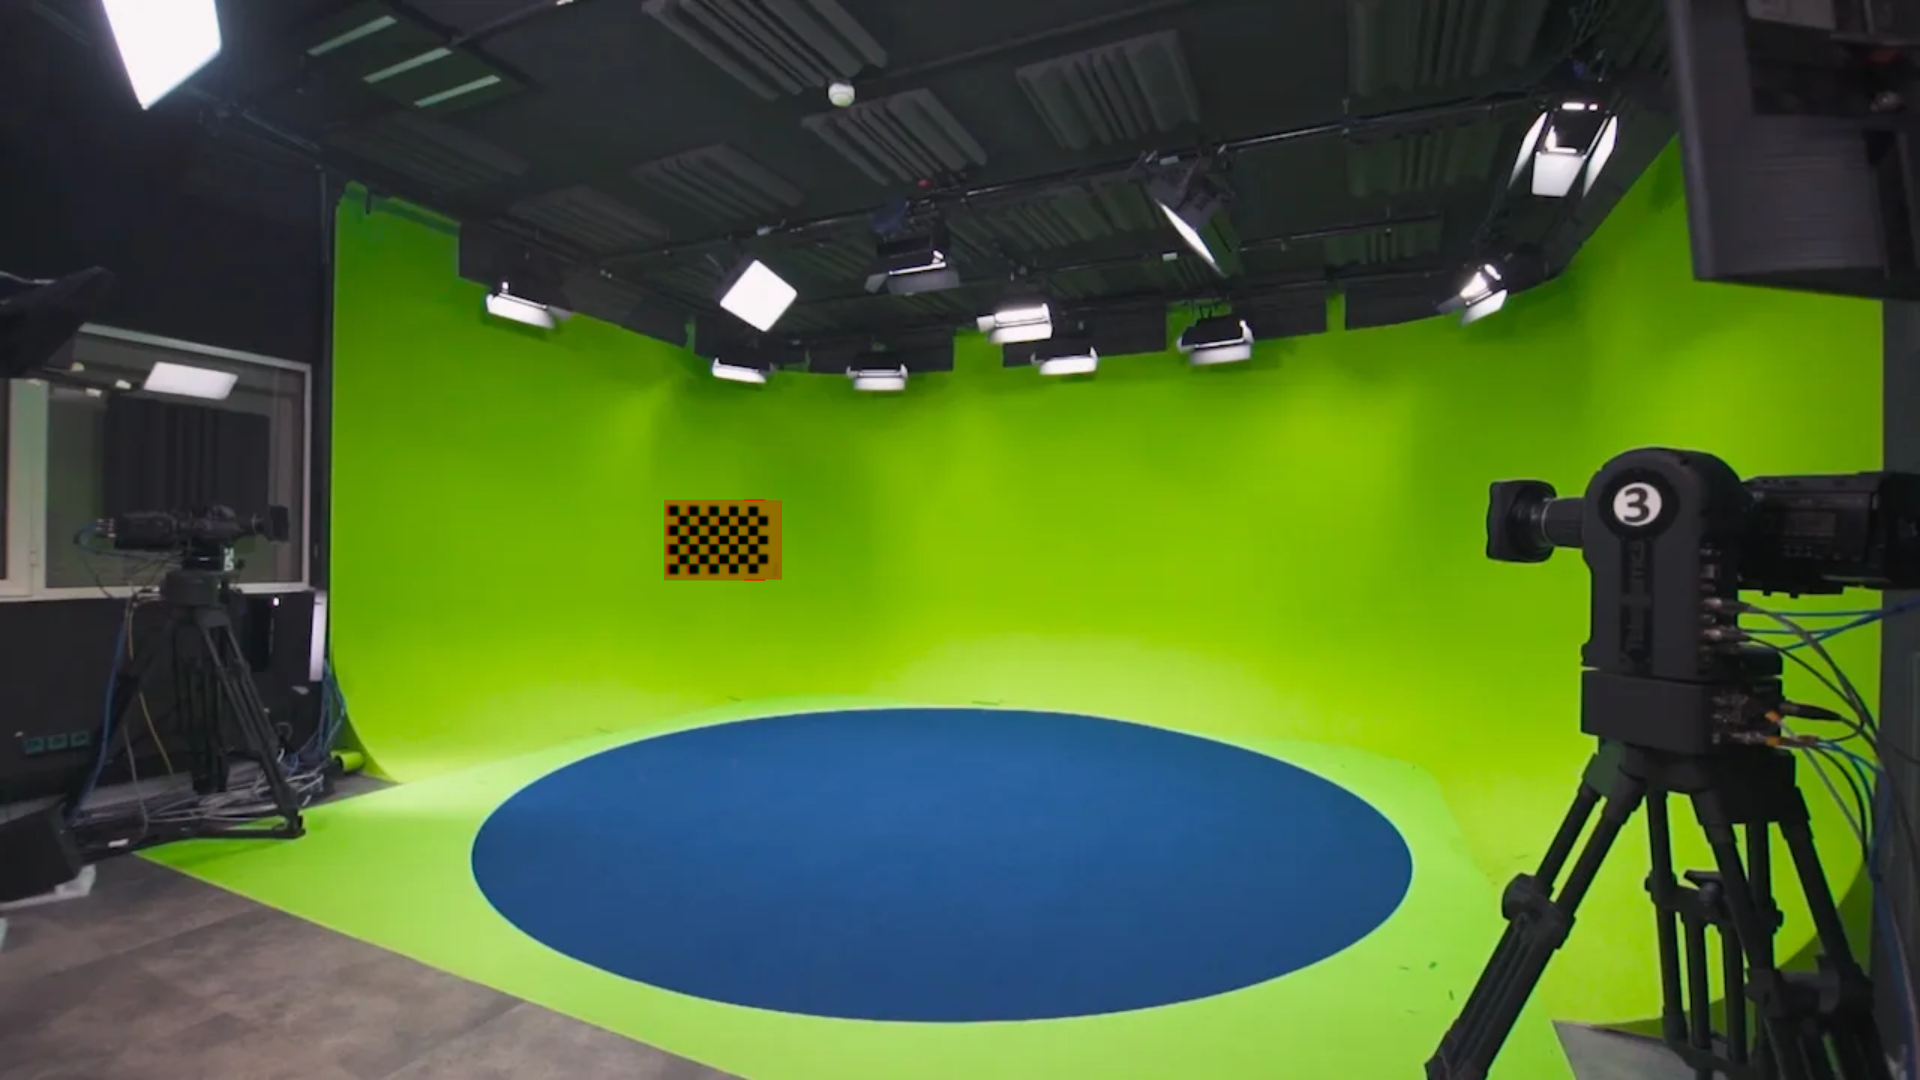
\includegraphics[width=\textwidth]{Images/08annex/results/2.2.png}
        \caption{}
        \label{fig:a2}
    \end{subfigure}
    \hfill
    \begin{subfigure}[b]{0.45\textwidth}
        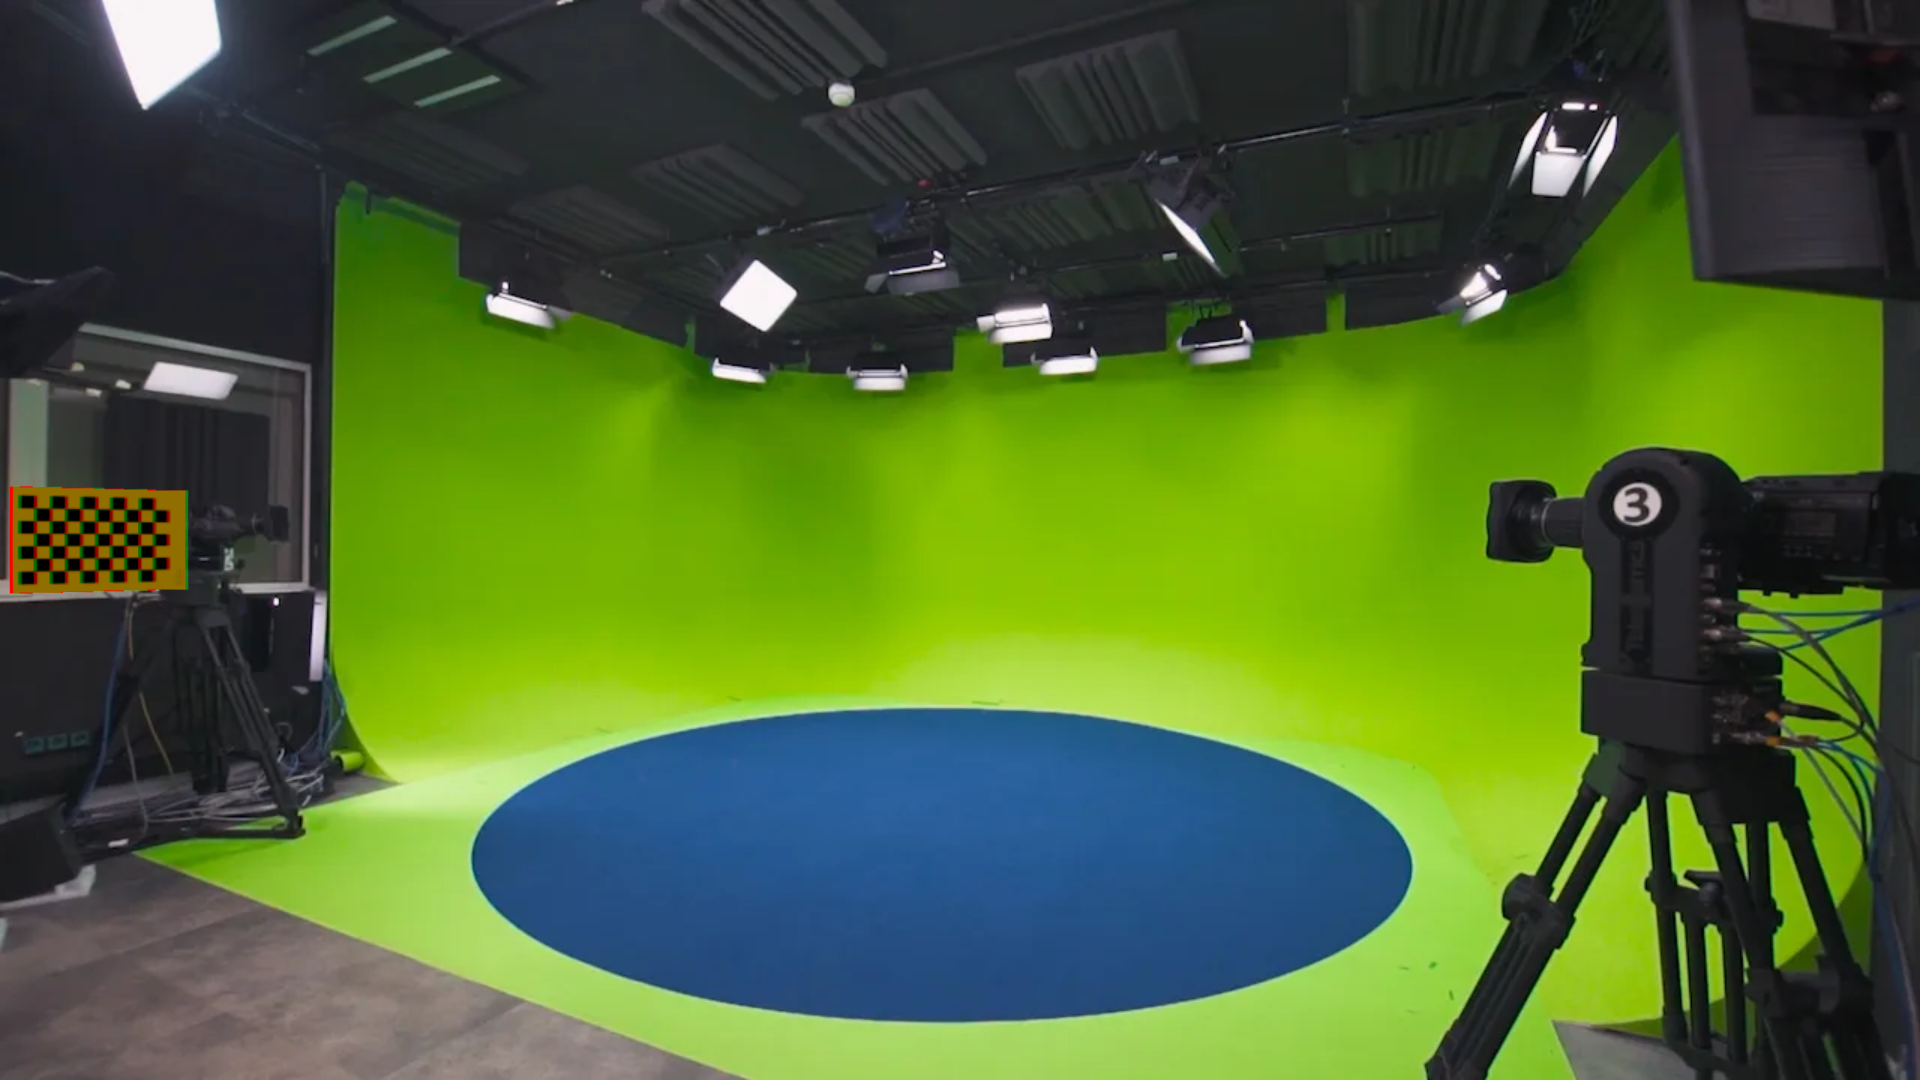
\includegraphics[width=\textwidth]{Images/08annex/results/2.3.png}
        \caption{}
        \label{fig:b2}
    \end{subfigure}
    
    \vspace{0.5cm}
    
    \begin{subfigure}[b]{0.45\textwidth}
        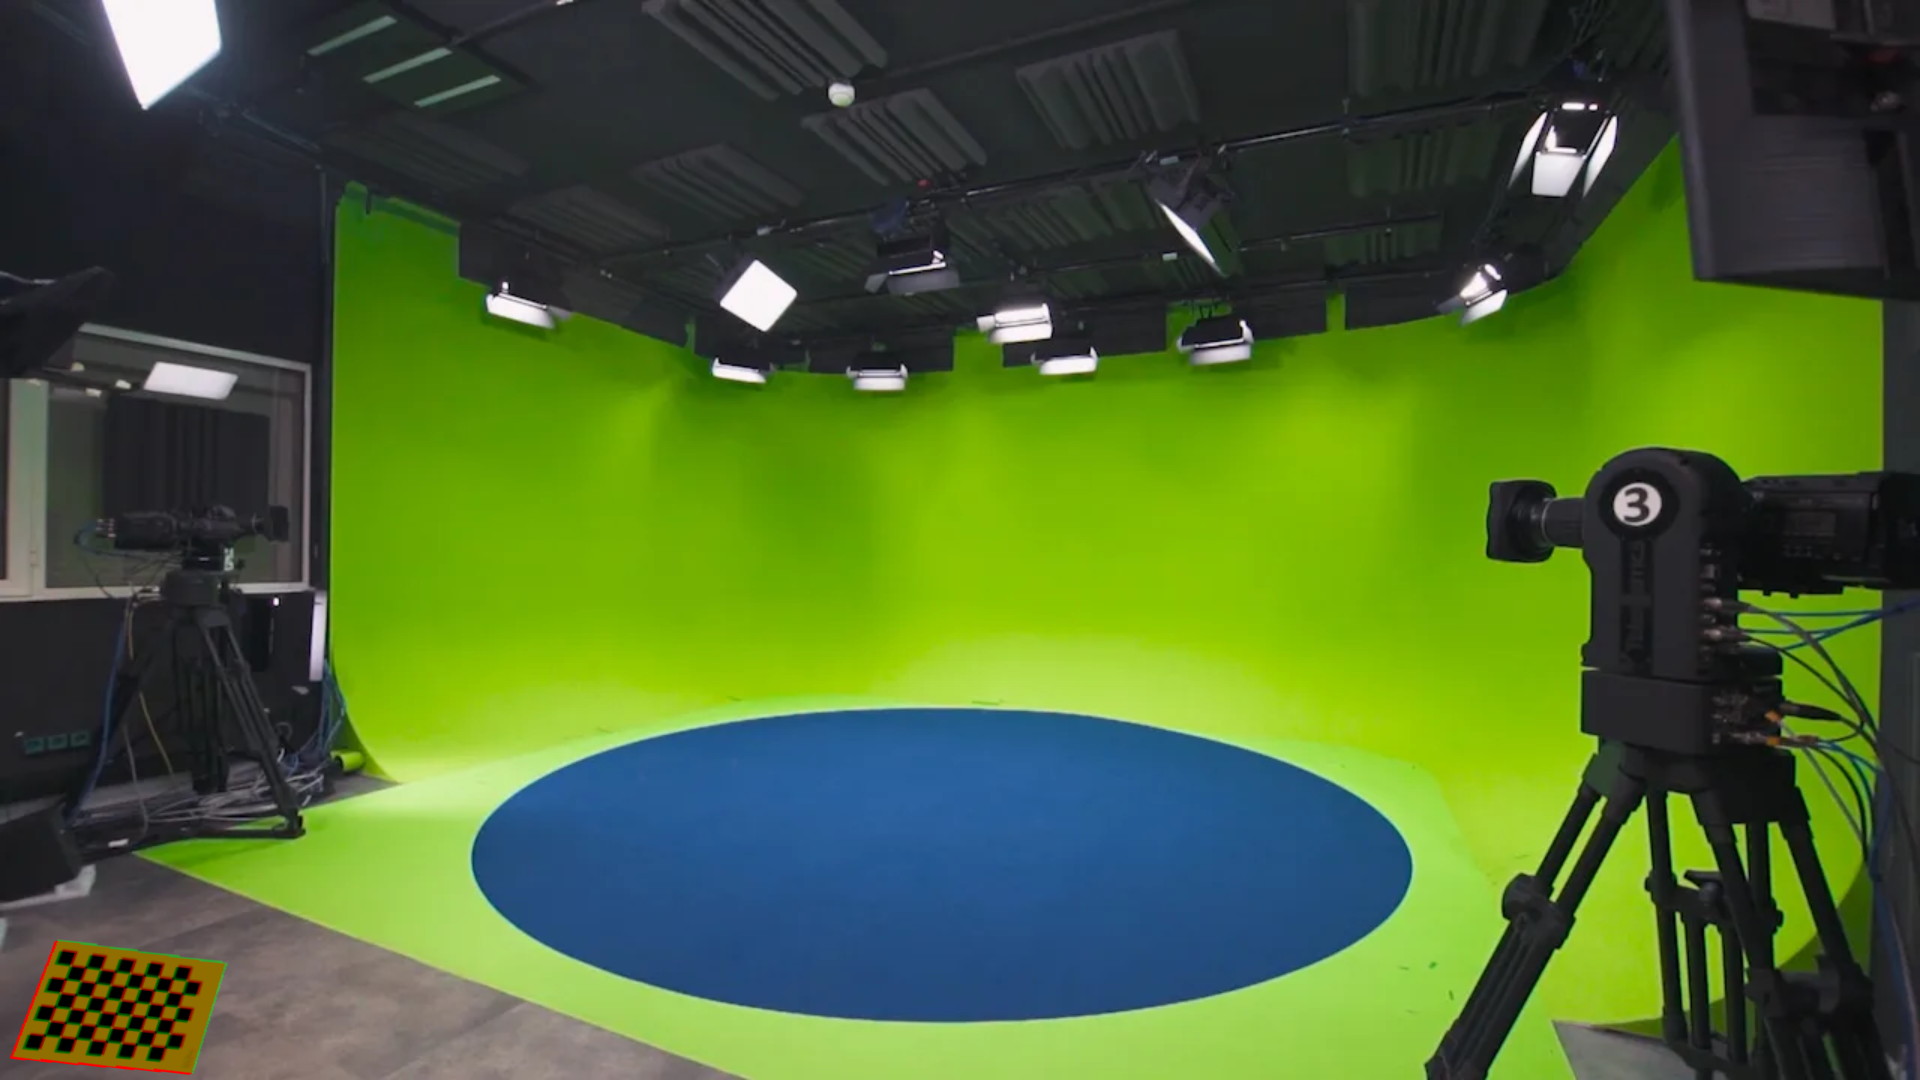
\includegraphics[width=\textwidth]{Images/08annex/results/2.4.png}
        \caption{}
        \label{fig:c2}
    \end{subfigure}

    \caption{Zoom 1 Focus 2 - (a) FoV, (b) K1, (c) K2.}
    \label{fig:vir_fov_cal}
\end{figure}

\begin{figure}[h]
    \centering
    \begin{subfigure}[b]{0.45\textwidth}
        \includegraphics[width=\textwidth]{Images/08annex/results/3.2.png}
        \caption{}
        \label{fig:a23}
    \end{subfigure}
    \hfill
    \begin{subfigure}[b]{0.45\textwidth}
        \includegraphics[width=\textwidth]{Images/08annex/results/3.3.png}
        \caption{}
        \label{fig:b2}
    \end{subfigure}
    
    \vspace{0.5cm}
    
    \begin{subfigure}[b]{0.45\textwidth}
        \includegraphics[width=\textwidth]{Images/08annex/results/3.4.png}
        \caption{}
        \label{fig:c2}
    \end{subfigure}

    \caption{Zoom 2 Focus 1 - (a) FoV, (b) K1, (c) K2.}
    \label{fig:vir_fov_cal}
\end{figure}

\begin{figure}[h]
    \centering
    \begin{subfigure}[b]{0.45\textwidth}
        \includegraphics[width=\textwidth]{Images/08annex/results/4.2.png}
        \caption{}
        \label{fig:a2}
    \end{subfigure}
    \hfill
    \begin{subfigure}[b]{0.45\textwidth}
        \includegraphics[width=\textwidth]{Images/08annex/results/4.3.png}
        \caption{}
        \label{fig:b2}
    \end{subfigure}
    
    \vspace{0.5cm}
    
    \begin{subfigure}[b]{0.45\textwidth}
        \includegraphics[width=\textwidth]{Images/08annex/results/4.4.png}
        \caption{}
        \label{fig:c2}
    \end{subfigure}

    \caption{Zoom 2 Focus 2 - (a) FoV, (b) K1, (c) K2.}
    \label{fig:vir_fov_cal}
\end{figure}

\begin{figure}[h]
    \centering
    \begin{subfigure}[b]{0.45\textwidth}
        \includegraphics[width=\textwidth]{Images/08annex/results/5.2.png}
        \caption{}
        \label{fig:a2}
    \end{subfigure}
    \hfill
    \begin{subfigure}[b]{0.45\textwidth}
        \includegraphics[width=\textwidth]{Images/08annex/results/5.3.png}
        \caption{}
        \label{fig:b2}
    \end{subfigure}
    
    \vspace{0.5cm}
    
    \begin{subfigure}[b]{0.45\textwidth}
        \includegraphics[width=\textwidth]{Images/08annex/results/5.4.png}
        \caption{}
        \label{fig:c2}
    \end{subfigure}

    \caption{Zoom 3 Focus 1 - (a) FoV, (b) K1, (c) K2.}
    \label{fig:vir_fov_cal}
\end{figure}

\begin{figure}[h]
    \centering
    \begin{subfigure}[b]{0.45\textwidth}
        \includegraphics[width=\textwidth]{Images/08annex/results/6.2.png}
        \caption{}
        \label{fig:a2}
    \end{subfigure}
    \hfill
    \begin{subfigure}[b]{0.45\textwidth}
        \includegraphics[width=\textwidth]{Images/08annex/results/6.3.png}
        \caption{}
        \label{fig:b2}
    \end{subfigure}
    
    \vspace{0.5cm}
    
    \begin{subfigure}[b]{0.45\textwidth}
        \includegraphics[width=\textwidth]{Images/08annex/results/6.4.png}
        \caption{}
        \label{fig:c2}
    \end{subfigure}

    \caption{Zoom 3 Focus 2 - (a) FoV, (b) K1, (c) K2.}
    \label{fig:vir_fov_cal}
\end{figure}

\begin{figure}[h]
    \centering
    \begin{subfigure}[b]{0.45\textwidth}
        \includegraphics[width=\textwidth]{Images/08annex/results/7.2.png}
        \caption{}
        \label{fig:a2}
    \end{subfigure}
    \hfill
    \begin{subfigure}[b]{0.45\textwidth}
        \includegraphics[width=\textwidth]{Images/08annex/results/7.3.png}
        \caption{}
        \label{fig:b2}
    \end{subfigure}
    
    \vspace{0.5cm}
    
    \begin{subfigure}[b]{0.45\textwidth}
        \includegraphics[width=\textwidth]{Images/08annex/results/7.4.png}
        \caption{}
        \label{fig:c2}
    \end{subfigure}

    \caption{Zoom 4 Focus 1 - (a) FoV, (b) K1, (c) K2.}
    \label{fig:vir_fov_cal}
\end{figure}

\begin{figure}[h]
    \centering
    \begin{subfigure}[b]{0.45\textwidth}
        \includegraphics[width=\textwidth]{Images/08annex/results/8.2.png}
        \caption{}
        \label{fig:a23}
    \end{subfigure}
    \hfill
    \begin{subfigure}[b]{0.45\textwidth}
        \includegraphics[width=\textwidth]{Images/08annex/results/8.3.png}
        \caption{}
        \label{fig:b2}
    \end{subfigure}
    
    \vspace{0.5cm}
    
    \begin{subfigure}[b]{0.45\textwidth}
        \includegraphics[width=\textwidth]{Images/08annex/results/8.4.png}
        \caption{}
        \label{fig:c2}
    \end{subfigure}

    \caption{Zoom 4 Focus 2 - (a) FoV, (b) K1, (c) K2.}
    \label{fig:vir_fov_cal}
\end{figure}

\begin{figure}[h]
    \centering
    \begin{subfigure}[b]{0.45\textwidth}
        \includegraphics[width=\textwidth]{Images/08annex/results/9.2.png}
        \caption{}
        \label{fig:a2}
    \end{subfigure}
    \hfill
    \begin{subfigure}[b]{0.45\textwidth}
        \includegraphics[width=\textwidth]{Images/08annex/results/9.3.png}
        \caption{}
        \label{fig:b2}
    \end{subfigure}
    
    \vspace{0.5cm}
    
    \begin{subfigure}[b]{0.45\textwidth}
        \includegraphics[width=\textwidth]{Images/08annex/results/9.4.png}
        \caption{}
        \label{fig:c2}
    \end{subfigure}

    \caption{Zoom 5 Focus 1 - (a) FoV, (b) K1, (c) K2.}
    \label{fig:vir_fov_cal}
\end{figure}

\begin{figure}[h]
    \centering
    \begin{subfigure}[b]{0.45\textwidth}
        \includegraphics[width=\textwidth]{Images/08annex/results/10.2.png}
        \caption{}
        \label{fig:a2}
    \end{subfigure}
    \hfill
    \begin{subfigure}[b]{0.45\textwidth}
        \includegraphics[width=\textwidth]{Images/08annex/results/10.3.png}
        \caption{}
        \label{fig:b2}
    \end{subfigure}
    
    \vspace{0.5cm}
    
    \begin{subfigure}[b]{0.45\textwidth}
        \includegraphics[width=\textwidth]{Images/08annex/results/10.4.png}
        \caption{}
        \label{fig:c2}
    \end{subfigure}

    \caption{Zoom 5 Focus 2 - (a) FoV, (b) K1, (c) K2.}
    \label{fig:vir_fov_cal}
\end{figure}

\begin{figure}[h]
    \centering
    \begin{subfigure}[b]{0.45\textwidth}
        \includegraphics[width=\textwidth]{Images/08annex/results/11.2.png}
        \caption{}
        \label{fig:a2}
    \end{subfigure}
    \hfill
    \begin{subfigure}[b]{0.45\textwidth}
        \includegraphics[width=\textwidth]{Images/08annex/results/11.3.png}
        \caption{}
        \label{fig:b2}
    \end{subfigure}
    
    \vspace{0.5cm}
    
    \begin{subfigure}[b]{0.45\textwidth}
        \includegraphics[width=\textwidth]{Images/08annex/results/11.4.png}
        \caption{}
        \label{fig:c2}
    \end{subfigure}

    \caption{Zoom 6 Focus 1 - (a) FoV, (b) K1, (c) K2.}
    \label{fig:vir_fov_cal}
\end{figure}

\begin{figure}[h]
    \centering
    \begin{subfigure}[b]{0.45\textwidth}
        \includegraphics[width=\textwidth]{Images/08annex/results/12.2.png}
        \caption{}
        \label{fig:a2}
    \end{subfigure}
    \hfill
    \begin{subfigure}[b]{0.45\textwidth}
        \includegraphics[width=\textwidth]{Images/08annex/results/12.3.png}
        \caption{}
        \label{fig:b2}
    \end{subfigure}
    
    \vspace{0.5cm}
    
    \begin{subfigure}[b]{0.45\textwidth}
        \includegraphics[width=\textwidth]{Images/08annex/results/12.4.png}
        \caption{}
        \label{fig:c2}
    \end{subfigure}

    \caption{Zoom 6 Focus 2 - (a) FoV, (b) K1, (c) K2.}
    \label{fig:vir_fov_cal}
\end{figure}

\begin{figure}[h]
    \centering
    \begin{subfigure}[b]{0.45\textwidth}
        \includegraphics[width=\textwidth]{Images/08annex/results/13.2.png}
        \caption{}
        \label{fig:a2}
    \end{subfigure}
    \hfill
    \begin{subfigure}[b]{0.45\textwidth}
        \includegraphics[width=\textwidth]{Images/08annex/results/13.3.png}
        \caption{}
        \label{fig:b2}
    \end{subfigure}
    
    \vspace{0.5cm}
    
    \begin{subfigure}[b]{0.45\textwidth}
        \includegraphics[width=\textwidth]{Images/08annex/results/13.4.png}
        \caption{}
        \label{fig:c2}
    \end{subfigure}

    \caption{Zoom 7 Focus 1 - (a) FoV, (b) K1, (c) K2.}
    \label{fig:vir_fov_cal}
\end{figure}



%% appendix
\appendix
%\include{Chapters/app1}

%% references
%\renewcommand{\bibname}{Referências} % o babel portuguese coloca Bibliografia
% os meses do ficheiro bib poderão aparecer em inglês, caso se pretenda deve-se colocar o texto em português explicitamente no ficheiro bid
\cleardoublepage%
\phantomsection%
\addcontentsline{toc}{chapter}{\bibname}
%\bibliographystyle{unsrtnat}
\bibliographystyle{plainnaturlAppear} % use plainnaturlAppear to order references by appearance 
% usually it is by author on thesis, to ease Author lookup
\nocite{*}  % Include all entries in references.bib, not just the ones cited.
\bibliography{references} %changed the env to make it a numbered chapter

%% bye
\end{document}
